\documentclass[11pt]{article}

%% ====================================================================
%% The Monetary-Financial-Fiscal Macromodel — user guide and methodology.
%% Style model: Ferroni & Canova (2021), "A hitchhiker's guide to
%% empirical macro models" (Chicago Fed WP 2021-15): methodology stated
%% with numbered equations and every symbol defined at first use, tool
%% usage interleaved with the theory, Examples and Remarks for practice,
%% derivations and tables in appendices.
%%
%% Accuracy contract: every equation in this document was checked against
%% the implementation (app/src/lib/compute/*, pipeline/*.m) at the time of
%% writing; file names are cited where the correspondence matters. The
%% per-economy tables in Appendix B are GENERATED from the shipped data
%% files by docs/generate_manual_tables.py -- regenerate, never hand-edit.
%%
%% Build: lualatex (or pdflatex) MFFM_User_Manual.tex; bibtex; 2x lualatex.
%% ====================================================================

\usepackage[margin=2.5cm]{geometry}
\usepackage{amsmath,amsfonts,amssymb,amsthm}
\usepackage{mathtools}
\usepackage{graphicx}
\usepackage{array}
\usepackage{booktabs,longtable}
\usepackage{pdflscape}
\usepackage[round,authoryear]{natbib}
\usepackage{hyperref}
\hypersetup{
  pdfpagelayout=OneColumn, pdfstartview=Fit, pdfpagemode=UseNone,
  colorlinks=true, citecolor=blue, filecolor=blue,
  linkcolor=blue, urlcolor=blue}
\usepackage{enumitem}
\usepackage{setspace}
\onehalfspacing
\usepackage{float}
\usepackage{caption}
\usepackage{xcolor}
% --- self-contained algorithm float (no texlive-science dependency) ---
\floatstyle{ruled}
\newfloat{algorithm}{!ht}{loa}
\floatname{algorithm}{Algorithm}
\newcounter{algstep}
\newenvironment{algsteps}
  {\begin{list}{\textbf{\arabic{algstep}:}}{\usecounter{algstep}%
     \setlength{\leftmargin}{2.0em}\setlength{\labelwidth}{1.6em}%
     \setlength{\itemsep}{1.5pt}\setlength{\parsep}{0pt}%
     \setlength{\topsep}{2pt}}}
  {\end{list}}
\newcommand{\algIn}[1]{\noindent\textbf{Input:} #1\par\vspace{1pt}}
\newcommand{\algOut}[1]{\noindent\textbf{Output:} #1\par\vspace{1pt}}
\newcommand{\algInd}{\hspace*{1.4em}}
\newcommand{\algIndd}{\hspace*{2.8em}}
\newcommand{\algKw}[1]{\textbf{#1}}
\newcommand{\algComment}[1]{{\color{black!55}\(\triangleright\) #1}}
% ----------------------------------------------------------------------
\usepackage{microtype}
\usepackage{tikz}
\usetikzlibrary{arrows.meta,positioning,fit,backgrounds,calc,decorations.pathreplacing}
\microtypesetup{expansion=false}

\newcommand{\R}{\mathbb{R}}
\newcommand{\E}{\mathbb{E}}
\newcommand{\Var}{\operatorname{Var}}
\newcommand{\diag}{\operatorname{diag}}
\newcommand{\cmark}{{\color{green!55!black}\checkmark}}
\newcommand{\xmark}{{\color{red!70!black}\ensuremath{\times}}}
% UI element: a button, toggle, or panel named exactly as on screen.
\newcommand{\ui}[1]{\textbf{#1}}

\theoremstyle{plain}
\newtheorem{example}{Example}
\theoremstyle{remark}
\newtheorem{remark}{Remark}

\begin{document}

%% ================================================================
%% TITLE PAGE
%% ================================================================
\begin{titlepage}
\vspace*{3cm}
\begin{center}
{\LARGE\bfseries A guide to the Monetary-Financial-Fiscal Macromodel:\\[4pt]
 conditional forecasts, global scenarios, and\\[2pt] policy counterfactuals in the browser}%
\footnote{The views expressed herein are those of the author and should
not be attributed to the International Monetary Fund, its Executive
Board, or its management.  The tool is provided ``as is'' without
warranty of any kind, express or implied.  The author and the IMF
disclaim all liability for any errors, omissions, or for any loss or
damage arising from its use.  Users are solely responsible for any
decisions made based on the output of this tool.}

\vspace{1.2cm}

{\large\itshape M\'aty\'as Farkas}\\[4pt]
International Monetary Fund

\vspace{1.5cm}

\today

\vspace{1.5cm}

Source code: \url{https://github.com/matyasfarkas/BVARScenarioTool}

\end{center}
\vfill
\end{titlepage}

%% ================================================================
%% ABSTRACT PAGE
%% ================================================================
\begin{center}
{\LARGE\bfseries A guide to the Monetary-Financial-Fiscal Macromodel}\\[6pt]
{\large conditional forecasts, global scenarios, and policy counterfactuals in the browser}
\end{center}

\vspace{0.6cm}
\begin{center}
M\'aty\'as Farkas\\
International Monetary Fund
\end{center}
\begin{center}
\today
\end{center}

\vspace{0.8cm}
\begin{center}\textbf{Abstract}\end{center}
\begin{quote}
This document describes the Monetary-Financial-Fiscal Macromodel, a browser-based
tool for quarterly macroeconomic projection and scenario analysis
covering about fifty economies. Each economy is a Bayesian vector
autoregression estimated with the hierarchical prior of
\citet{Giannone2015} under a COVID-as-missing data-augmentation
treatment; thirty-three of them are coupled into a global system with an
endogenous United States, solved as a linear fixed point at display
time. The user conditions any subset of variables on hard or soft paths
--- a mouse drag, an imported outside forecast with a chosen degree of
trust --- and a Durbin--Koopman smoother
\citep{DurbinKoopman2002} propagates the constraints to every other
variable and, on request, across borders. Public debt and the external
position are derived from the estimated drivers by their accounting
identities; long-run anchors shift the companion drift exactly and
instantly; and monetary or fiscal counterfactuals are evaluated with
impulse responses from the Macroeconomic Model Data Base
\citep{WielandCwikMuellerSchmidtWolters2012}. We state the methods with
their exact implemented conventions, show how each is operated from the
interface, and document the data, the out-of-sample evaluation, and the
replication path. All computation runs client-side; there is no server.
\end{quote}

\vspace{0.4cm}
\noindent\textbf{Keywords}: BVARs, Conditional Forecasting, GVAR, Missing
Values, Scenario Analysis, Kalman Filter, Policy Counterfactuals, DSGE
Models

\vspace{0.2cm}
\noindent\textbf{JEL classification}: C32, C53, E37, E52, E58, F47

\vfill
\noindent\rule{\textwidth}{0.4pt}\\[4pt]
{\footnotesize Email: \texttt{mfarkas@imf.org}. I am grateful to Jesper
Lind\'e for comments, advice, and continued support throughout the
development of this tool, and to Tobias Adrian for his support. The
views and any remaining errors are my own.}

\clearpage
\tableofcontents
\clearpage

%% ================================================================
\section{Introduction}\label{sec:intro}
%% ================================================================

The tool described in this document is a single web page. It loads the
estimated models of about fifty economies into the browser and lets the
user read, bend, and export their quarterly forecasts. There is nothing
to install and no server-side computation: every number on the screen is
produced client-side, so the tool can be hosted as a static website and
used offline once loaded. The source code, the estimation pipeline, and
the data files are in one repository,
\begin{center}
\url{https://github.com/matyasfarkas/BVARScenarioTool}
\end{center}
with the deployed application served from its \texttt{app/} static
export. The tool comes as is; it is a research platform, not an official
forecast of any institution.

The economic machinery is organized in three layers, applied in order:
\begin{enumerate}[label=(\roman*)]
  \item \textbf{Baseline.} Each economy is an $n$-variable Bayesian
    vector autoregression (BVAR) estimated on quarterly data with the
    hierarchical Minnesota prior of \citet{Giannone2015}, treating the
    pandemic quarters as missing data
    (Section~\ref{sec:bvar}). Thirty-three economies are additionally
    coupled into a global VAR (GVAR) with a fully endogenous United
    States (Section~\ref{sec:gvar}). The baseline forecast is computed
    once, offline, and shipped with the model.
  \item \textbf{Scenario.} The user conditions any subset of variables
    on desired paths. Conditioning is a partial-observation problem in
    the companion-form state space, solved by a Kalman filter and
    Durbin--Koopman smoother \citep{BanburaGiannoneLenza2015,
    DurbinKoopman2002}; a pinned value can be \emph{hard} (exact) or
    \emph{soft} (an outside forecast held with a chosen degree of
    trust), and it propagates to the other variables --- and, on
    request, to the other economies --- through the estimated covariance
    and trade structure (Sections~\ref{sec:cond} and~\ref{sec:gvar}).
  \item \textbf{Counterfactual.} A monetary or fiscal policy
    counterfactual is overlaid on the scenario using impulse responses
    from a DSGE model of the user's choice, drawn from the Macroeconomic
    Model Data Base \citep[MMB;][]{WielandCwikMuellerSchmidtWolters2012},
    and re-conditioned through the BVAR so the remaining variables stay
    consistent with the estimated co-movements
    (Section~\ref{sec:counterfactual}).
\end{enumerate}
On top of these, two accounting blocks derive what should not be
estimated freely: public debt from the budget identity
(Section~\ref{sec:fiscal}) and the net external position from the
balance-of-payments identity (Section~\ref{sec:external}); and a
long-run anchor mechanism shifts the far end of any forecast onto a
user-chosen value, exactly and instantly (Section~\ref{sec:longrun}).

Three display rules govern everything on screen, and we state them here
because the rest of the document relies on them. \emph{Data are data}:
observed history is drawn solid; any model-filled value --- a not-yet-published
quarter estimated from everything already observed --- is drawn in amber
and labelled, never disguised as an observation. \emph{The model is
frozen within the year}: quarterly data updates advance the forecast
origin but never silently change the estimated coefficients;
re-estimation happens once a year on a complete final year of data
(Section~\ref{sec:data}). \emph{Judgment is visible}: whenever the user
moves a forecast away from the model --- a scenario pin, a long-run
target, a counterfactual --- the chart says so with a badge.

This document is both the user guide and the methodological
documentation. It is organized so that each section states a method with
its exact implemented conventions --- the equations below were checked
against the code, and file names are cited where the correspondence
matters --- and then shows how that method is operated from the
interface, in numbered Examples that name the on-screen controls
exactly. Section~\ref{sec:start} gets a new user from a blank page to a
first scenario. Sections~\ref{sec:bvar}--\ref{sec:cond} cover the
estimation and the conditional-forecasting engine,
Section~\ref{sec:gvar} the cross-country system,
Sections~\ref{sec:fiscal}--\ref{sec:external} the accounting blocks,
Section~\ref{sec:longrun} the long-run anchors, and
Section~\ref{sec:counterfactual} the policy counterfactuals.
Section~\ref{sec:data} documents the data and the vintage policy,
Section~\ref{sec:eval} the out-of-sample evaluation,
Section~\ref{sec:impl} the implementation and the replication path, and
Section~\ref{sec:final} concludes with limitations and known issues.
Notation is collected in Appendix~\ref{app:notation}; the per-economy
variable tables --- generated directly from the deployed data files ---
are Appendix~\ref{app:tables}; a glossary is Appendix~\ref{app:glossary}.

%% ================================================================
\begin{figure}[!ht]
\centering
\resizebox{\textwidth}{!}{%
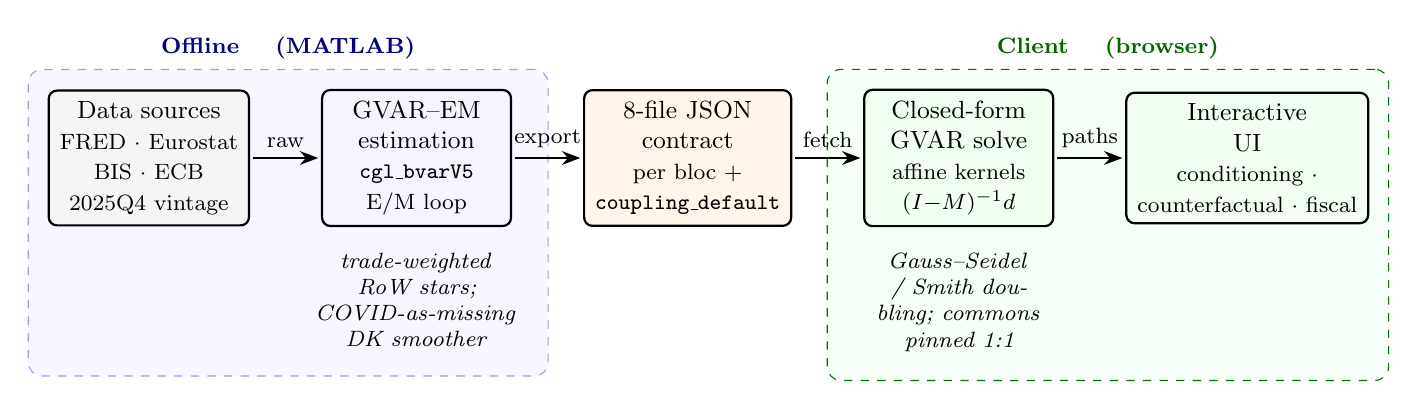
\begin{tikzpicture}[
  font=\small,
  >=Stealth,
  node distance=9mm,
  stage/.style={
    rounded corners=3pt, draw, thick, align=center,
    minimum height=15mm, minimum width=24mm, inner sep=4pt,
    fill=blue!4
  },
  data/.style={stage, fill=gray!8},
  contract/.style={stage, fill=orange!8},
  client/.style={stage, fill=green!6},
  flow/.style={->, thick, shorten >=1pt, shorten <=1pt},
  bandlbl/.style={font=\footnotesize\itshape}
]

% ---- stages, left to right ----
\node[data] (src) {Data sources\\\footnotesize FRED $\cdot$ Eurostat\\\footnotesize BIS $\cdot$ ECB\\\footnotesize 2025Q4 vintage};
\node[stage, right=of src] (est) {GVAR--EM\\estimation\\\footnotesize \texttt{cgl\_bvarV5}\\\footnotesize E/M loop};
\node[contract, right=of est] (json) {8-file JSON\\contract\\\footnotesize per bloc $+$\\\footnotesize \texttt{coupling\_default}};
\node[client, right=of json] (solve) {Closed-form\\GVAR solve\\\footnotesize affine kernels\\\footnotesize $(I{-}M)^{-1}d$};
\node[client, right=of solve] (ui) {Interactive\\UI\\\footnotesize conditioning $\cdot$\\\footnotesize counterfactual $\cdot$ fiscal};

% ---- flow arrows with labels ----
\draw[flow] (src) -- node[above, font=\footnotesize] {raw} (est);
\draw[flow] (est) -- node[above, font=\footnotesize] {export} (json);
\draw[flow] (json) -- node[above, font=\footnotesize] {fetch} (solve);
\draw[flow] (solve) -- node[above, font=\footnotesize] {paths} (ui);

% ---- under-arrows: methodological annotations ----
\node[below=2mm of est, bandlbl, text width=26mm, align=center] (estsub)
  {trade-weighted RoW stars; COVID-as-missing DK smoother};
\node[below=2mm of solve, bandlbl, text width=26mm, align=center] (solvesub)
  {Gauss--Seidel / Smith doubling; commons pinned 1:1};

% ---- background bands: offline (MATLAB) vs client (browser) ----
\begin{scope}[on background layer]
  \node[fit=(src)(est)(estsub), draw=blue!40, dashed, rounded corners=5pt,
        fill=blue!3, inner sep=7pt,
        label={[blue!55!black,font=\footnotesize\bfseries]above:Offline \quad (MATLAB)}] (offband) {};
  \node[fit=(solve)(ui)(solvesub), draw=green!45!black, dashed, rounded corners=5pt,
        fill=green!4, inner sep=7pt,
        label={[green!40!black,font=\footnotesize\bfseries]above:Client \quad (browser)}] (clband) {};
\end{scope}

\end{tikzpicture}%
}
\caption[End-to-end system architecture]{End-to-end system architecture of the EM-Bayesian Global VAR platform.
Harmonized macro-financial data (FRED, Eurostat, BIS, ECB; common 2025Q4 \emph{estimation} vintage, with
the observed panel subsequently refreshed to 2026Q1 with no re-estimation, \S\ref{sec:data}) feed the
\emph{offline} MATLAB GVAR--EM estimator: per-bloc Bayesian VARs (\texttt{cgl\_bvarV5}) are re-fit in an
EM loop that, at each sweep, rebuilds the trade-weighted rest-of-world ``star'' variables
(ROWDEM/ROWINF/ROWFIN) from partners' Durbin--Koopman-completed panels and re-estimates every bloc with
the 2020Q2--Q4 \emph{macro} columns masked (the foreign-rate star ROWFIN and all domestic financials kept
observed; COVID-as-missing), iterating to $\max|\Delta\text{star}|<0.03$ (cf.\ \S\ref{sec:gvarem}). Each
converged bloc is serialized to the eight-file JSON contract (\texttt{spec}, \texttt{companion\_mean},
\texttt{companion\_draws}, \texttt{baseline}, \texttt{baseline\_levels}, \texttt{historical},
\texttt{historical\_levels}, \texttt{transformations}; plus \texttt{fiscal\_meta} and the precomputed
\texttt{coupling\_default.json.gz} coupling artifact). In the \emph{client} (browser), the cross-country
system is solved in closed form: the scenario delta obeys the affine fixed point $x = Mx + d$, evaluated by
Gauss--Seidel sweeps or directly via $(I-M)^{-1}d$ (Smith doubling), with global commons (US WTI oil,
US~10Y, US~BAA, US~equity) pinned 1:1 onto every RoW bloc. The interactive UI exposes conditioning,
counterfactuals, and the stock-flow fiscal block (\S\ref{sec:fiscal}).}
\label{fig:architecture}
\end{figure}
\section{Getting started}\label{sec:start}
%% ================================================================

\subsection{The screen}\label{sec:screen}

\begin{figure}[!ht]
\centering
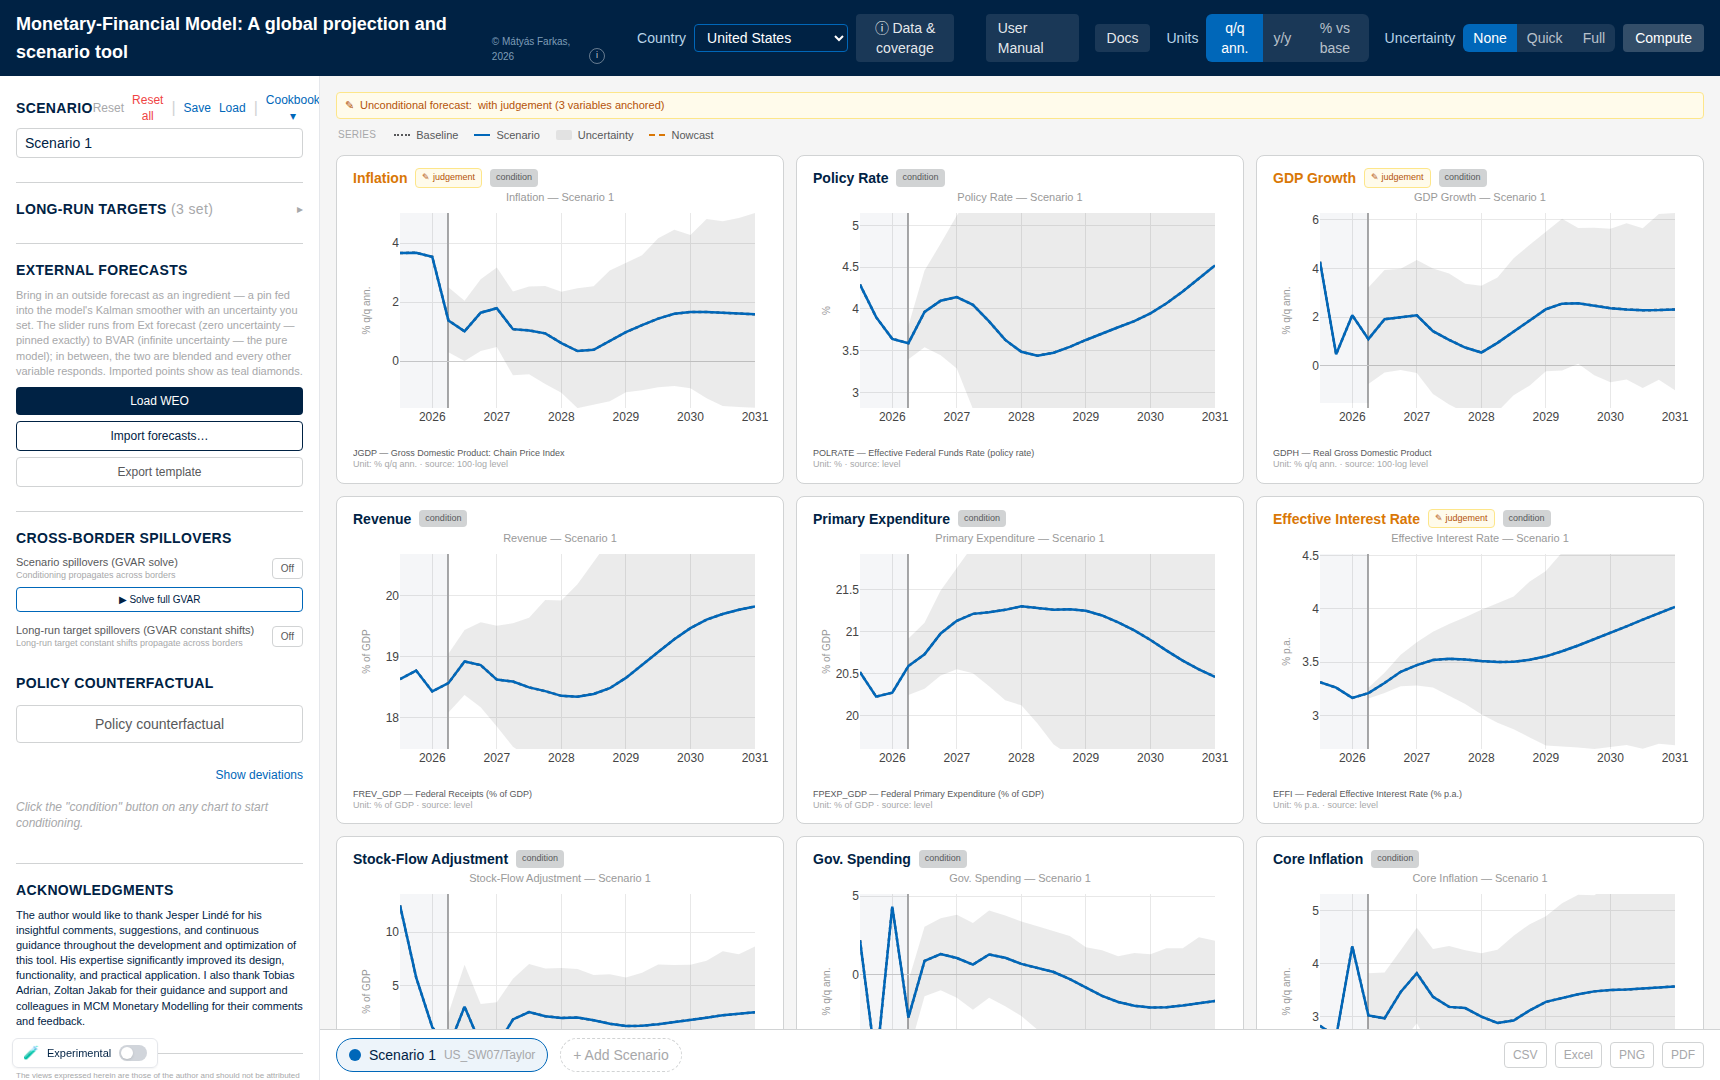
\includegraphics[width=\textwidth]{manual_figs/ui_overview.png}
\caption{The screen at load (United States). The top bar holds the country selector, the
\emph{Data \& coverage} provenance panel, the display-unit toggles (q/q annualized, y/y, \% vs
base), the uncertainty setting (None/Quick/Full), and \textsf{Compute}. The left rail holds the
scenario manager, long-run targets, external forecasts (\S\ref{sec:external-fc}), cross-border
spillovers (\S\ref{sec:gvarusage}), and the policy counterfactual
(\S\ref{sec:counterfactual}). Each chart shows history, the dotted baseline, the solid scenario
path, and the predictive band; \textsf{judgement} chips mark anchored variables
(\S\ref{sec:longrun}) and every chart carries a \textsf{condition} chip
(\S\ref{sec:pinusage}).}
\label{fig:ui-overview}
\end{figure}


Open the tool's address in a modern browser and give the first visit a
few seconds; the model files load into the page. The screen has four
parts:
\begin{itemize}
  \item the \emph{top bar}: the \ui{Country} dropdown, the display
    \ui{Units} toggle, the \ui{Uncertainty} switch
    (\ui{None}/\ui{Quick}/\ui{Full}), the \ui{Compute} button, the
    \ui{Data \& coverage} dialog, and links to this manual, the online
    documentation (\ui{Docs}), and the release-impact \ui{Monitor};
  \item the \emph{left control panel}: the \ui{Scenario} block (with
    \ui{Reset}, \ui{Reset all}, \ui{Save}, \ui{Load}, and the
    \ui{Cookbook} of ready-made scenarios), \ui{Long-run targets},
    \ui{External forecasts}, \ui{Cross-border spillovers}, the
    \ui{Policy Counterfactual} block, and --- once a variable is
    conditioned --- the quarter-by-quarter conditioning list;
  \item the \emph{chart grid}: one chart per variable; this is where
    the user clicks and drags;
  \item the \emph{scenario bar} along the bottom: one tab per scenario
    (up to four, \ui{+ Add Scenario}) and the \ui{CSV}, \ui{Excel},
    \ui{PNG}, and \ui{PDF} export buttons.
\end{itemize}
The \ui{Country} dropdown has two groups. Economies under \ui{GVAR}
belong to the coupled cross-country system of Section~\ref{sec:gvar}; a
scenario built there can reach every other member. Economies under
\ui{Other countries} --- including the individual euro-area member
states, which receive shocks through the euro-area aggregate
(Section~\ref{sec:eamembers}) --- are forecast on their own. Switching
country never deletes work: each economy keeps its scenario settings
until reset.

\subsection{Reading one chart}\label{sec:readchart}

Every chart follows the same grammar, and reading it correctly is most
of the tool:
\begin{itemize}
  \item \emph{History} sits on a lightly shaded background; the solid
    line there is observed data. If a series' latest quarters have not
    been published, its history ends in an \emph{amber dashed} tail with
    open circles --- model-filled values (a \emph{nowcast},
    Section~\ref{sec:vintage}), never disguised as data. Hovering one
    reads \emph{Model-implied nowcast (imputed)}.
  \item The \emph{dotted grey line} is the \ui{Baseline}: the model's
    own forecast, untouched by the user. The pale grey fan around it is
    the model's predictive uncertainty, shipped with the estimation
    (Section~\ref{sec:bands}); it is there before anything is computed.
  \item The \emph{solid coloured line} is the active scenario. Until the
    user conditions something it lies exactly on the baseline.
  \item The \emph{header} carries a \ui{condition} button (click to make
    the variable steerable; it turns into \ui{CONDITIONED}), a
    \ui{derived} badge on charts computed by an accounting identity, and
    an amber \ui{judgement} badge whenever a long-run target has moved
    the variable off the model's estimate.
  \item The \emph{footer} gives the variable's definition and unit.
\end{itemize}

The \ui{Units} toggle changes the lens, not the numbers:
\ui{q/q ann.}\ is the quarter-on-quarter annualized rate (the model's
native display unit, equation~\eqref{eq:growth} below); \ui{y/y} the
change on the same quarter a year earlier; \ui{\% vs base} the
\emph{difference} between scenario and baseline, centred at zero --- a
read-only impact view in which a second toggle, \ui{Level} versus
\ui{Rate (IRF)}, selects between the cumulative level effect and the
quarter-by-quarter response (Section~\ref{sec:cfread}). Charts that are
already rates (the policy rate, unemployment) ignore the toggle, and a
handful of index series (oil, exchange-rate, equity, and house-price
indices) are always drawn as levels, because a trade-weighted index
quoted q/q-annualized is not an informative number.

\begin{example}[A first scenario in five minutes]\label{ex:first}
Open the tool; the \ui{Country} dropdown reads \ui{United States}, with
\ui{Units} on \ui{q/q ann.}\ and \ui{Uncertainty} on \ui{None}.
(1)~On the \ui{Policy Rate} chart click \ui{condition}; the button turns
blue and reads \ui{CONDITIONED}. (2)~Press the mouse on the forecast
region about four quarters out and drag half a percentage point above
the dotted baseline; release. A dot marks the pinned quarter, and the
solid scenario line passes through it --- only that quarter is imposed,
and the model fills in the most plausible route through the point.
(3)~Scroll the grid: every chart has updated, not just the rate ---
growth cools, inflation eases with a lag --- because the smoother
re-draws the whole forecast consistently with the pin
(Section~\ref{sec:cond}). Other countries have not moved;
cross-border transmission is off until requested
(Section~\ref{sec:gvarusage}). (4)~Set \ui{Uncertainty} to \ui{Quick}
and press \ui{Compute}: after a few seconds a band in the scenario's
colour wraps the solid line --- the middle two-thirds of plausible
outcomes --- and collapses onto the line at the pinned quarter, because
an imposed value carries no uncertainty
(Section~\ref{sec:scenbands}). (5)~Clean up: in the left panel click
\ui{Reset} (clears the active scenario for this country only) and set
\ui{Uncertainty} back to \ui{None}. A right-click on an unconditioned
chart is the shortcut for steps (1)--(2): it conditions the variable and
plants the pin at the cursor in one gesture.
\end{example}

\begin{remark}[When to press Compute]\label{rem:compute}
The central scenario path updates live with every pin; \ui{Compute} is
never needed to see it. The button exists for the two calculations that
are too heavy to run on every mouse move: the scenario uncertainty bands
(Section~\ref{sec:scenbands}) and the complete cross-country solve
(Section~\ref{sec:gvarusage}). It is greyed out until either
\ui{Quick}/\ui{Full} uncertainty is selected or a long-run target is
set. Bands are a snapshot --- change a pin afterwards and the band no
longer matches until \ui{Compute} is pressed again.
\end{remark}

%% ================================================================
\section{The country models}\label{sec:bvar}
%% ================================================================

\subsection{Reduced form and data spaces}\label{sec:spaces}

Each economy (``bloc'') $c$ is an $n$-variable VAR with $p$ lags in
reduced form,
\begin{equation}\label{eq:var}
  y_t = c + \sum_{\ell=1}^{p} B_\ell\, y_{t-\ell} + u_t,
  \qquad u_t \sim \mathcal{N}(0, \Sigma),
\end{equation}
where $y_t \in \R^n$ collects the bloc's observables, $c \in \R^n$ is
the intercept, $B_\ell \in \R^{n\times n}$ are the autoregressive
matrices, and $\Sigma \in \R^{n\times n}$ is the innovation covariance.
Throughout, $p=3$ and the forecast horizon is $H=20$ quarters. The
deployed dimensions run from $n=16$ (Costa Rica) to $n=40$ (the United
States); Appendix~\ref{app:tables} tabulates every bloc. The estimated
coefficients are stored as a $(1+np)\times n$ matrix $\hat\beta$ whose
\emph{first} row is the intercept and whose remaining $np$ rows stack
the lag coefficients $[B_1;\dots;B_p]$ --- a convention the reader needs
only twice, for the companion construction~\eqref{eq:companion} and the
model signature of Section~\ref{sec:modelsig}.

Variables enter the VAR in one of two spaces, recorded per variable in
the bloc's specification (\texttt{spec.json}) and never changed at run
time:
\begin{itemize}
  \item \texttt{log}: the stored series is $\ell_t = 100\ln Y_t$.
    Displayed growth is quarter-on-quarter annualized,
    \begin{equation}\label{eq:growth}
      g_t \;=\; 4\,(\ell_t - \ell_{t-1}) \;=\; 400\,(\ln Y_t - \ln Y_{t-1}),
    \end{equation}
    and year-on-year growth is $\ell_t - \ell_{t-4}$. The factor of
    $4$ on the stored $100\ln$ space --- never $400$, which would
    re-apply the $100$ --- is the single most load-bearing convention in
    the tool; every pin, band, and cross-country link below respects it.
  \item \texttt{lin}: the series enters in levels (interest rates in
    percent, unemployment, ratios to GDP). No growth conversion is
    applied.
\end{itemize}
Display units are chosen per variable for readability: activity and
price series are shown as growth and inflation via~\eqref{eq:growth};
rates and ratios as levels in percent; and index series (the
trade-weighted dollar, equity, house prices, oil, commodity indices) as
the index level $\exp(\ell_t/100)$, with conditioning still performed in
the stored $100\ln$ space. Unemployment-rate bands are floored at zero;
policy-rate bands are not, since negative nominal rates occur.

\subsection{The hierarchical prior}\label{sec:prior}

Estimation follows the hierarchical approach of \citet{Giannone2015},
henceforth GLP: the Minnesota prior
\citep{Litterman1986, DoanLittermanSims1984} with its tightness treated
as a hyperparameter and selected by maximizing the marginal likelihood.
The prior centers each equation on a univariate own-lag model, with a
sum-of-coefficients component \citep{DoanLittermanSims1984} shrinking
toward ``a unit increase in every level raises its own forecast one for
one.'' Two hyperparameters are sampled --- the overall tightness
$\lambda$ and the sum-of-coefficients weight $\mu$ --- by a
random-walk Metropolis step on the marginal likelihood of the
\emph{completed} data (Section~\ref{sec:covid}), initialized at the
\texttt{csminwel} optimum; the remaining prior settings are held at
their GLP defaults. The estimator is the bundled MATLAB implementation
(\texttt{BVAR/MFBVAR/bvarGLPmf.m}, called through the COVID-aware
wrapper \texttt{cgl\_bvarV5.m}); no external MATLAB packages are
required.

\paragraph{Own-lag prior mean: random walk or white noise.}\label{sec:ownlag}
The prior mean on variable $i$'s own first lag is $\delta_i$, with
$\delta_i = 1$ (random walk, \texttt{RW}) the default: for
(near-)integrated series --- log activity, log prices, nominal yields
--- ``the best forecast of the level is the current level.'' For a
genuinely \emph{stationary} series, a mean-reverting ratio that
fluctuates around a constant, the random-walk center is the wrong null:
it shrinks toward a unit root and lets the projection drift at long
horizons. Such variables carry \texttt{prior:"WN"} in the specification
and are estimated with $\delta_i = 0$ (white noise): ``the best forecast
is the unconditional mean.'' The mechanism is one line in the prior
construction --- the own-lag prior-mean diagonal is zeroed at the
\texttt{WN} indices (\texttt{diagb(pos)=0} in \texttt{bvarGLPmf.m}, with
\texttt{pos} built from the per-variable tags) --- and it moves only the
prior \emph{center}, not a hard constraint: a persistent series whose
data favour a near-unit root still obtains a large posterior own-lag
coefficient at the estimated tightness. In the deployed panel the
\texttt{WN} tag is carried by the three fiscal GDP-ratios
(Section~\ref{sec:fiscal}); every other variable is \texttt{RW}
(Appendix~\ref{app:tables}).

\subsection{Seasonal dummies}\label{sec:seasonal}

A subset of the panel is reported \emph{not seasonally adjusted}, so a
regular quarter-of-year cycle sits in the level: NSA consumer prices
(HICP/CPI for several economies and euro members), unemployment rates,
house-price indices, India's government series, and the UK and Korean
stock-flow adjustments. Left untreated, a pure autoregression can
reproduce such a cycle only through a near-unit root close to the
seasonal frequency, which then \emph{explodes} the projection into a
spurious sawtooth out of sample. The deterministic remedy is a set of
quarterly dummies. For a bloc flagged seasonal, let
$q(t)\in\{1,2,3,4\}$ be the calendar quarter of observation $t$ and
collect the three non-base indicators
\begin{equation}\label{eq:seasdummy}
  D_t = \bigl[\,\mathbf{1}\{q(t)=2\},\ \mathbf{1}\{q(t)=3\},\
              \mathbf{1}\{q(t)=4\}\,\bigr],
\end{equation}
with the first quarter as the base. Each equation's regressor vector
becomes $x_t = [\,1,\ D_t,\ y_{t-1}',\dots,y_{t-p}'\,]$, so the
estimated coefficient block acquires three deterministic rows between
the constant and the lag matrices,
\begin{equation}\label{eq:betalayout}
  \widehat{\beta}
   = \bigl[\,\underbrace{c}_{1};\
             \underbrace{\gamma_{Q2};\ \gamma_{Q3};\ \gamma_{Q4}}_{n_{\mathrm{sr}}=3};\
             \underbrace{B_1;\dots;B_p}_{n\,\text{lag blocks}}\,\bigr],
  \qquad k = 1 + n_{\mathrm{sr}} + n\,p,
\end{equation}
where $n$ is the number of endogenous variables, $p=3$ the lag order,
and $n_{\mathrm{sr}}$ the number of ``seasonal rows'' ($3$ when the bloc
is flagged, $0$ otherwise --- the legacy layout, left byte-identical).
The dummy coefficients $\gamma_{Q2},\gamma_{Q3},\gamma_{Q4}$ carry a
\emph{diffuse} prior --- the intercept variance $V_c$, centred at zero
--- and are zeroed in the sum-of-coefficients dummy observations, so the
shrinkage machinery treats them like the constant and never pulls them
toward a unit root (\texttt{BVAR/MFBVAR/Support/BVAR.m}; the COVID-aware
wrapper \texttt{cgl\_bvarV5.m} passes them through the \texttt{qoy}
argument and carries the seasonal term in the simulation-smoother
artificial path, so the Durbin--Koopman completion of
Section~\ref{sec:covid} stays exact).

Which blocs are flagged is data-driven: a panel scan tags a bloc
seasonal when at least one series shows calendar-$R^2 \ge 0.40$ with a
display amplitude $\ge 2$, and every coupon-lumpy bloc of
Remark~\ref{rem:evencoupon} is added because its \texttt{SFA} inherits
the cash-versus-accrual timing. In the deployed system this is sixteen
coupled blocs (CL, CN, CO, CR, EA, ID, IL, IN, IS, JP, KR, MX, NO, TR,
UK, ZA) and six euro members (ES, IT, GR, PT, SI, BE); all remaining
blocs keep $n_{\mathrm{sr}}=0$.

In the projection the three coefficients generate a \emph{bounded},
repeating quarter-of-year cycle rather than an explosive root: the tool
precomputes four quarter-specific transition constants and picks the one
matching each forecast step's quarter-of-year phase
(\texttt{c2ByQ}/\texttt{c2AtStep} in
\texttt{app/src/lib/compute/kalman.ts}). The phase itself is always
recomputed from the tool's own date grid --- the quarter following the
last history point, wrapped $1\!\dots\!4$ --- never read from the shipped
estimation-grid value, which sits one quarter behind after the
production data shift. Every $n_{\mathrm{sr}}=0$ path is unchanged to the
byte.

\subsection{COVID as missing data}\label{sec:covid}

The 2020 pandemic quarters are extreme outliers that would otherwise
contaminate both the autoregressive coefficients and $\Sigma$. Rather
than dummying or rescaling them, the estimator treats the pandemic
window as \emph{missing} and imputes it inside the estimation, by a
data-augmentation Gibbs sampler in the sense of \citet{TannerWong1987}:
each sweep alternates
\begin{enumerate}[label=(\roman*)]
  \item a Durbin--Koopman simulation-smoother draw
    \citep{DurbinKoopman2002} of the missing cells given the current
    coefficients, treating them as \texttt{NaN} observations in the
    companion-form state space of Section~\ref{sec:ss}
    (Algorithm~\ref{alg:dksmoother});
  \item a Metropolis--Hastings update of $(\lambda,\mu)$ on the
    completed-data marginal likelihood; and
  \item a draw of $(\beta,\Sigma)$ from the completed data.
\end{enumerate}
The surrounding quarters stay in the sample and inform the imputation,
so the pandemic history is preserved while the outlier does not drive
the dynamics.

Two implementation choices matter. First, the production window is the
\emph{fixed} three quarters 2020Q2--Q4 for every bloc. (A legacy
single-bloc variant self-calibrates the window to the GDP trough
searched within 2019Q4--2021Q1 --- restricting the search matters, since
an unrestricted trough lands on the wrong crisis for some economies,
e.g.\ Korea's 2008Q4 --- but the deployed GVAR estimator uses the fixed
window.) Second, the masking is \emph{macro-only}: over the window the
domestic macro columns and the two macro star variables of
Section~\ref{sec:stars} are set missing, while the financial columns
(rates, yields, equity, house prices, spreads; the \texttt{isFinancial}
tag in Appendix~\ref{app:tables}) and the financial star stay
\emph{observed}. The smoother therefore imputes the pandemic macro holes
conditional on financial series that carry genuine signal through 2020.
The same device handles non-pandemic artefacts: the UK effective-rate
spike of 2008--09, a mechanical consequence of inflation uplift on
index-linked gilts being recorded as accrued interest, is NaN'd and
imputed identically (Section~\ref{sec:fiscal}).

\begin{algorithm}[!ht]
\caption{Durbin--Koopman simulation smoother with partial observations
(one draw inside the data-augmentation Gibbs sweep;
\texttt{cgl\_bvarV5.m}).}
\label{alg:dksmoother}
\algIn{system matrices $T, Z, Q$ of Section~\ref{sec:ss}; partial
observations $\{y_t^{(o)}\}$ (COVID-masked and ragged cells absent);
current draw of $(\beta,\Sigma)$.}
\algOut{one draw $\tilde\alpha_{1:T}$ from
$p(\alpha_{1:T}\mid y^{(o)},\beta,\Sigma)$, hence imputed values for the
missing cells.}
\begin{algsteps}
\item \algComment{(1) Forward simulation of an unconditional path.}
\item Draw $\alpha_0^{+}$ from the initial law; \algKw{for}
  $t=1,\dots,T$: draw shocks and set
  $\alpha_t^{+}=T\alpha_{t-1}^{+}+\eta_t$, $y_t^{+}=Z\alpha_t^{+}$.
\item Form synthetic partial observations $y_t^{+(o)}$ on the
  \emph{same} missing pattern as the data.
\item \algComment{(2) Kalman filter (Section~\ref{sec:kf}) on the
  artificial series $y_t^{(o)}-y_t^{+(o)}$, processing only the observed
  rows at each date.}
\item \algComment{(3) Backward smoothing recursion
  (equation~\eqref{eq:dk} of Section~\ref{sec:kf}) $\Rightarrow$ smoothed
  discrepancy $\hat\alpha_t$.}
\item \algComment{(4) Mean correction.}
  $\tilde\alpha_t \gets \alpha_t^{+} + \hat\alpha_t$; read the imputed
  cells off $\tilde y_t = Z\tilde\alpha_t$.
\end{algsteps}
\end{algorithm}

\subsection{What ships: posterior output and predictive bands}\label{sec:bands}

For the deterministic engine the posterior is summarized by the means
$(\hat\beta, \hat\Sigma)$. For uncertainty the chain is thinned to
$D = 500$ retained draws $\{(\hat\beta^{(d)}, \hat\Sigma^{(d)})\}$,
shipped per bloc in \texttt{companion\_draws.json} and loaded lazily ---
only when the user first presses \ui{Compute} (the US file is the
largest at roughly 34\,MB).

The shipped baseline carries \emph{predictive} bands, not
parameter-only bands: the Gibbs sampler emits a forecast density that
integrates over parameter uncertainty, future innovations, and the
missing-data imputation simultaneously, and the exported quantiles are
\begin{equation}\label{eq:bands}
  \bigl(q_{05},\,q_{16},\,q_{50},\,q_{84},\,q_{95}\bigr)_{T+h}
  \;=\; \mathrm{Quantile}\bigl\{\, \tilde{y}^{(d)}_{T+h} \,\bigr\}_{d=1}^{D},
\end{equation}
drawn on the charts as the grey fan (the 68\% band $(q_{16},q_{84})$
shaded, the 90\% band $(q_{05},q_{95})$ fainter). The \emph{central}
path remains the deterministic forecast from the posterior means, so an
untouched screen shows the stored baseline exactly. Scenario bands ---
computed in the browser, conditional on the user's pins --- are
constructed differently and are described with the conditioning engine
(Section~\ref{sec:scenbands}).

Every bloc is serialized to one eight-file JSON contract ---
\texttt{spec}, \texttt{companion\_mean}, \texttt{companion\_draws},
\texttt{baseline}, \texttt{baseline\_levels}, \texttt{historical},
\texttt{historical\_levels}, \texttt{transformations} --- fiscal blocs
adding \texttt{fiscal\_meta} and external blocs
\texttt{external\_meta}, with
every float compacted to six significant figures. The deployed
application reads only this contract and never re-estimates
(Section~\ref{sec:impl}).

%% ================================================================
\section{Conditional forecasting}\label{sec:cond}
%% ================================================================

Conditioning a forecast on a chosen path is, in state-space form, the
same problem as filtering with missing data: a pinned cell is an
\emph{observation} of the future, a free cell is a missing one
\citep{BanburaGiannoneLenza2015, WaggonerZha1999}. This section states
the state space, the filter and smoother exactly as implemented
(\texttt{app/src/lib/compute/kalman.ts}), the display construction, and
the two kinds of pin --- hard and soft --- the interface exposes.

\subsection{Companion-form state space}\label{sec:ss}

Stack the current and lagged observables into the state
$\alpha_t = (y_t', y_{t-1}', \dots, y_{t-p+1}')' \in \R^{np}$. The
VAR~\eqref{eq:var} is then the first-order system
\begin{equation}\label{eq:ss}
  \alpha_t = T\,\alpha_{t-1} + c_\alpha + \eta_t,
  \qquad
  y_t = Z\,\alpha_t + \varepsilon_t,
\end{equation}
with
\begin{equation}\label{eq:companion}
  T = \begin{pmatrix}
    B_1 & B_2 & \cdots & B_{p-1} & B_p \\
    & I_{n(p-1)} & & & 0
  \end{pmatrix},
  \qquad
  c_\alpha = \begin{pmatrix} c \\ 0 \end{pmatrix},
  \qquad
  Z = \bigl(I_n \mid 0_{n \times n(p-1)}\bigr),
\end{equation}
$\eta_t \sim \mathcal{N}(0, Q)$ where $Q$ carries $\Sigma$ in its
top-left $n\times n$ block and zeros elsewhere, and
$\varepsilon_t \sim \mathcal{N}(0, R)$ with
\begin{equation}\label{eq:R}
  R = \sigma^2_\varepsilon I_n, \qquad \sigma^2_\varepsilon = 10^{-12}.
\end{equation}
The top block of $T$ is filled from the stored coefficients as
$T_{ij} = \hat\beta_{j+1,\,i}$ (the transpose of the lag rows, skipping
the intercept row), and $c_\alpha$ from the intercept row. The
measurement variance~\eqref{eq:R} is the \emph{hard-pin} noise: small
enough that a pinned value is honoured to machine precision, nonzero for
numerical stability. The state is initialized at the last $p$ observed
rows, $\alpha_0 = (y_T', \dots, y_{T-p+1}')'$, with
$P_0 = 10^{-7} I_{np}$.

\subsection{Filter and smoother with partial observations}\label{sec:kf}

\begin{figure}[!ht]
\centering
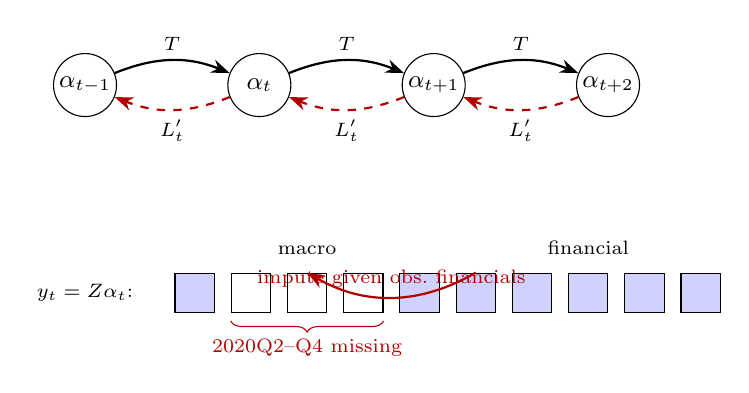
\begin{tikzpicture}[
    >=Stealth,
    font=\small,
    state/.style={circle,draw,minimum size=8mm,inner sep=0pt},
    obsfill/.style={rectangle,draw,minimum size=5mm,inner sep=0pt,fill=blue!18},
    obshollow/.style={rectangle,draw,minimum size=5mm,inner sep=0pt,fill=white},
    filt/.style={->,draw=black,thick},
    smth/.style={->,draw=red!70!black,thick,dashed},
    node distance=14mm,
]
% ---- state timeline ----
\node[state] (a1) {$\alpha_{t-1}$};
\node[state,right=of a1] (a2) {$\alpha_{t}$};
\node[state,right=of a2] (a3) {$\alpha_{t+1}$};
\node[state,right=of a3] (a4) {$\alpha_{t+2}$};

% forward Kalman filter (transition T) above
\draw[filt] (a1) to[bend left=22] node[above,font=\scriptsize]{$T$} (a2);
\draw[filt] (a2) to[bend left=22] node[above,font=\scriptsize]{$T$} (a3);
\draw[filt] (a3) to[bend left=22] node[above,font=\scriptsize]{$T$} (a4);

% backward DK smoother below
\draw[smth] (a4) to[bend left=22] node[below,font=\scriptsize]{$L_{t}'$} (a3);
\draw[smth] (a3) to[bend left=22] node[below,font=\scriptsize]{$L_{t}'$} (a2);
\draw[smth] (a2) to[bend left=22] node[below,font=\scriptsize]{$L_{t}'$} (a1);

% ---- observation row (COVID window 2020Q2--Q4) ----
\node[below=20mm of a1,anchor=north] (lab) {\scriptsize $y_t = Z\alpha_t$:};
% macro cells (hollow over the 3 COVID quarters)
\node[obsfill,right=4mm of lab] (m1) {};
\node[obshollow,right=2mm of m1] (m2) {};
\node[obshollow,right=2mm of m2] (m3) {};
\node[obshollow,right=2mm of m3] (m4) {};
\node[obsfill,right=2mm of m4]  (m5) {};
% financial cells (filled throughout)
\node[obsfill,right=2mm of m5] (f1) {};
\node[obsfill,right=2mm of f1] (f2) {};
\node[obsfill,right=2mm of f2] (f3) {};
\node[obsfill,right=2mm of f3] (f4) {};
\node[obsfill,right=2mm of f4] (f5) {};

\node[above=1mm of m3,font=\scriptsize] {macro};
\node[above=1mm of f3,font=\scriptsize] {financial};
% COVID bracket under the 3 missing macro cells
\draw[decorate,decoration={brace,amplitude=4pt,mirror},red!70!black]
   ($(m2.south west)+(0,-1mm)$) -- ($(m4.south east)+(0,-1mm)$)
   node[midway,below=3pt,font=\scriptsize,red!70!black]{2020Q2--Q4 missing};

% imputation arrow: observed financials -> imputed (hollow) macro hole
\draw[->,red!70!black,thick] (f1.north) to[bend left=30]
   node[above,font=\scriptsize]{impute given obs.\ financials} (m3.north);
\end{tikzpicture}
\caption{Companion-form state space with the Durbin--Koopman
filter/smoother under the COVID-as-missing treatment.  States
$\alpha_t$ (\S\ref{sec:ss}) evolve forward through the transition
matrix $T$ (solid, Kalman filter, Eq.~\eqref{eq:kfpred}); the
backward smoother propagates
$r_{t-1}=(Z_t^{(o)})'F_t^{-1}v_t+L_t'r_t$
(dashed, Eq.~\eqref{eq:dk}).  In the observation row
$y_t=Z\alpha_t$ (\S\ref{sec:ss}), over the fixed window
2020Q2--Q4 (three quarters) the \emph{macro} cells (real activity,
prices, and the macro stars ROWDEM/ROWINF) are set missing (hollow)
while the \emph{financial} cells (rates, yields, equity, house prices,
and the foreign-rate star ROWFIN) remain observed (filled).  Because
the filter processes only the observed rows $Z_t^{(o)}$ of each
partially-observed vector, the macro holes are imputed conditional on
the observed financials.}
\label{fig:statespace-dk}
\end{figure}

Collect the user's pins in a matrix $Y^{\ast} \in \R^{H\times n}$ with
$Y^{\ast}_{t,j}$ the pinned value of variable $j$ at forecast quarter
$t$ and \texttt{NaN} where free. At each $t$ the filter processes only
the observed rows: let $Z_t$ stack the rows of $Z$ for the pinned cells
(plus any linear-combination rows, below) and $R_t$ the corresponding
diagonal of measurement variances. For $t = 1,\dots,H$:
\begin{align}
  a_{t|t-1} &= T\, a_{t-1|t-1} + c_\alpha,
  &P_{t|t-1} &= T\, P_{t-1|t-1}\, T' + Q, \label{eq:kfpred}\\
  v_t &= y^{\ast}_t - Z_t\, a_{t|t-1},
  &F_t &= Z_t\, P_{t|t-1}\, Z_t' + R_t, \label{eq:kfinnov}\\
  K_t &= P_{t|t-1}\, Z_t'\, F_t^{-1},
  &a_{t|t} &= a_{t|t-1} + K_t\, v_t,
  \qquad
  P_{t|t} = P_{t|t-1} - K_t\, Z_t\, P_{t|t-1}, \label{eq:kfupd}
\end{align}
with $a_{t|t}=a_{t|t-1}$, $P_{t|t}=P_{t|t-1}$ at quarters with no pins.
$F_t^{-1}$ is computed by LU decomposition with partial pivoting
(singularity threshold $10^{-15}$), and the covariance updates are
symmetrized. The Durbin--Koopman fixed-interval smoother then runs
backward with $r_H = 0$:
\begin{equation}\label{eq:dk}
  L_t = T\bigl(I - P_{t|t-1} Z_t' F_t^{-1} Z_t\bigr), \qquad
  r_{t-1} = Z_t' F_t^{-1} v_t + L_t'\, r_t,
\end{equation}
($r_{t-1} = T' r_t$ at pin-free quarters), and the smoothed state is
$\hat\alpha_{t|H} = a_{t|t-1} + P_{t|t-1}\, r_{t-1}$. The smoothed
\emph{variance} is delivered by the companion $N$-recursion,
\begin{equation}\label{eq:Nrec}
  N_{t-1} = Z_t' F_t^{-1} Z_t + L_t'\, N_t\, L_t, \qquad
  V_t = P_{t|t-1} - P_{t|t-1}\, N_{t-1}\, P_{t|t-1},
\end{equation}
with $N_H = 0$; $V_t$ is the state covariance conditional on \emph{all}
pins, so uncertainty about a quarter \emph{preceding} a future pin is
correctly reduced by it. The conditional forecast is the observation
block of $\hat\alpha_{t|H}$; the display shading of the impact view
(Section~\ref{sec:scenbands}) reads $V_t$.

\paragraph{Linear-combination pins.} A constraint on a linear
combination $h'y_t = v$ --- used by the fiscal block to pin the primary
balance, $h_{\text{rev}} = +1$, $h_{\text{pexp}} = -1$
(Section~\ref{sec:fiscal}) --- enters the same machinery as one extra
observation row $(h'Z,\, v)$ with measurement variance
$\sum_k h_k^2\,\sigma^2_\varepsilon$. No separate variable is created.

\subsection{The display: exact deltas on the stored baseline}\label{sec:delta}

To guarantee that an untouched screen reproduces the shipped baseline
exactly, the tool displays
\begin{equation}\label{eq:delta}
  \hat{y}^{\text{display}}_{T+h}
  = \bar{y}^{\text{baseline}}_{T+h}
  + \bigl(\hat{y}^{\text{cond}}_{T+h} - \hat{y}^{\text{uncond}}_{T+h}\bigr),
\end{equation}
the stored baseline plus the smoother \emph{delta} between a conditional
and an unconditional pass (the latter cached and reused). Zero pins give
a zero delta and hence the stored baseline to the last digit. For
\texttt{log} variables the delta is computed in the $100\ln$ level space
and scaled to displayed growth by the factor $4$
of~\eqref{eq:growth}; a dragged growth pin is correspondingly cumulated
into the level pin, one quarter's worth ($\text{deviation}/4$) per
active quarter.

\subsection{Operating hard pins}\label{sec:pinusage}

\begin{figure}[!ht]
\centering
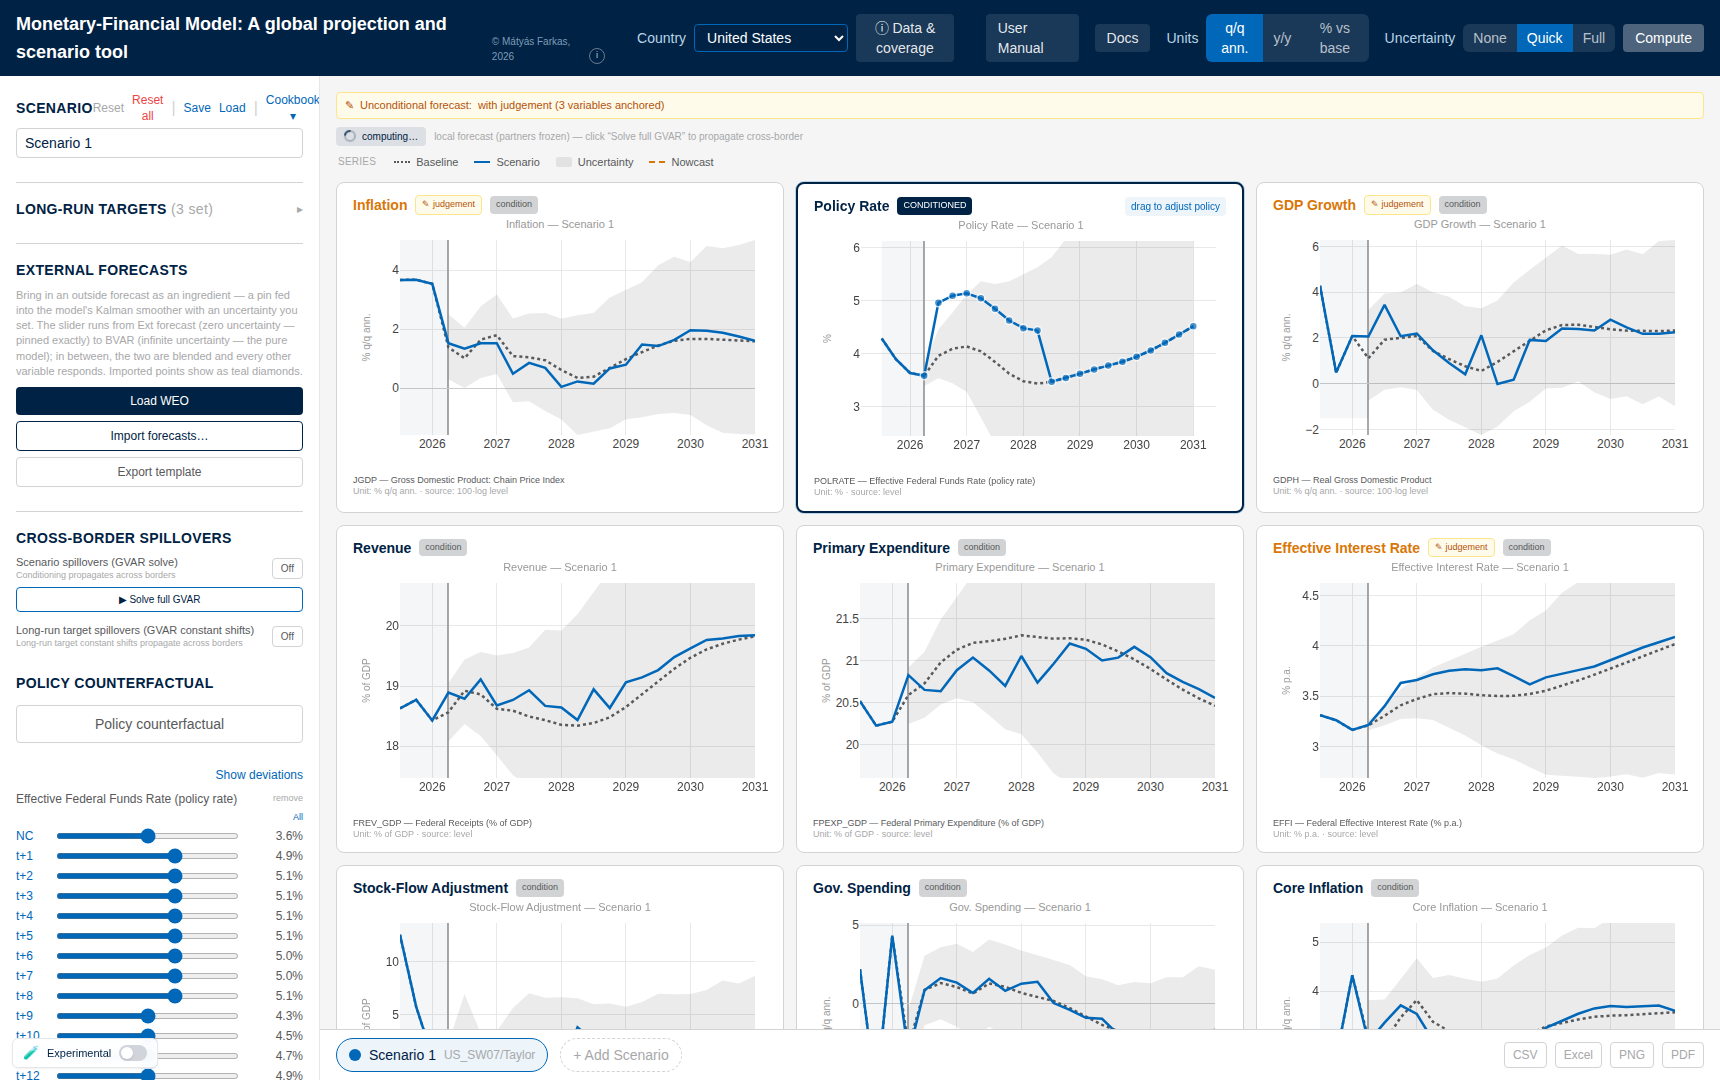
\includegraphics[width=\textwidth]{manual_figs/ui_conditioning.png}
\caption{Hard conditioning in action. The policy-rate chart is put in \textsf{CONDITIONED} mode and
the path is raised by $+100$\,bp for eight quarters --- by dragging the dots on the chart or the
per-quarter sliders that appear in the left rail (here $t{+}1,\dots,t{+}8$). After
\textsf{Compute}, every panel redraws the smoothed scenario (solid) against the frozen baseline
(dotted): output growth dips, inflation eases, the effective interest rate on debt climbs, and
the fiscal ratios respond --- all through the estimated cross-correlations of
\S\ref{sec:kf}; nothing is re-estimated.}
\label{fig:ui-conditioning}
\end{figure}


A pin is set on the chart (drag on a \ui{CONDITIONED} chart;
right-click to condition and plant in one gesture; right-click again to
toggle a quarter's pin off) or in the conditioning list, which shows one
row per forecast quarter, labelled \ui{NC}, \ui{t+1}, \dots, \ui{t+19}.
\ui{NC} --- the nowcast --- is the current, not-yet-published quarter
(Section~\ref{sec:vintage}). Each row has an on/off toggle and a value
slider; \ui{Show deviations}/\ui{Show levels} switches between entering
distances from baseline and absolute values. Pins are
what-you-set-is-what-you-see: a pinned quarter sits exactly at its
number, always; the quarters left off are filled by the model. Multiple
variables stack, and all pins are imposed \emph{jointly} --- the
smoother finds the single most plausible forecast through every pin at
once, so mutually strained pins show their cost in the unconditioned
charts. Up to four scenarios can be held side by side (the bottom bar);
\ui{Reset} clears the active scenario for the current country,
\ui{Reset all} everything everywhere, and \ui{Save}/\ui{Load} round-trip
one country's conditioning to an Excel file.

\begin{example}[A ready-made scenario, and what identification buys]\label{ex:cookbook}
The \ui{Cookbook} (left panel, \ui{Scenario} header) loads documented,
source-calibrated scenarios; each recipe offers \ui{Load naive} ---
pin only the headline variable --- and \ui{Load + restriction} --- add
the short-run pins that shape the shock into its economically meaningful
form. The credit-crunch recipe (calibrated to the Federal Reserve's 2020
severely-adverse scenario) illustrates on the United States what the
extra pins buy. \emph{Naive}: pin only the corporate bond yield $+400$bp.
The model reads a corporate-yield spike as generic rates tightening ---
the whole curve rises (at the 2026Q1 vintage, the policy rate peaks
around $7\tfrac12$\%, the 10-year near $8\tfrac12$\%) and inflation
moves \emph{up} on impact: comovement alone cannot tell a credit-supply
dislocation from a broad rate shift. \emph{Restricted}: add the
documented crunch signature --- safe 10-year yield \emph{down}
(flight to safety), output down, inflation down, equity down, the policy
rate cut. The same $+400$bp spread now produces a deep recession
(GDP trough near $-6$\% q/q ann.), disinflation, and easing --- the
policy rate and the safe yield move in the \emph{opposite} direction
from the naive read. Loading a recipe \emph{replaces} the active
scenario's pins; run the two variants on two scenario tabs to compare.
\end{example}

\subsection{Soft pins: outside forecasts with a trust dial}\label{sec:external-fc}

\begin{figure}[!ht]
\centering
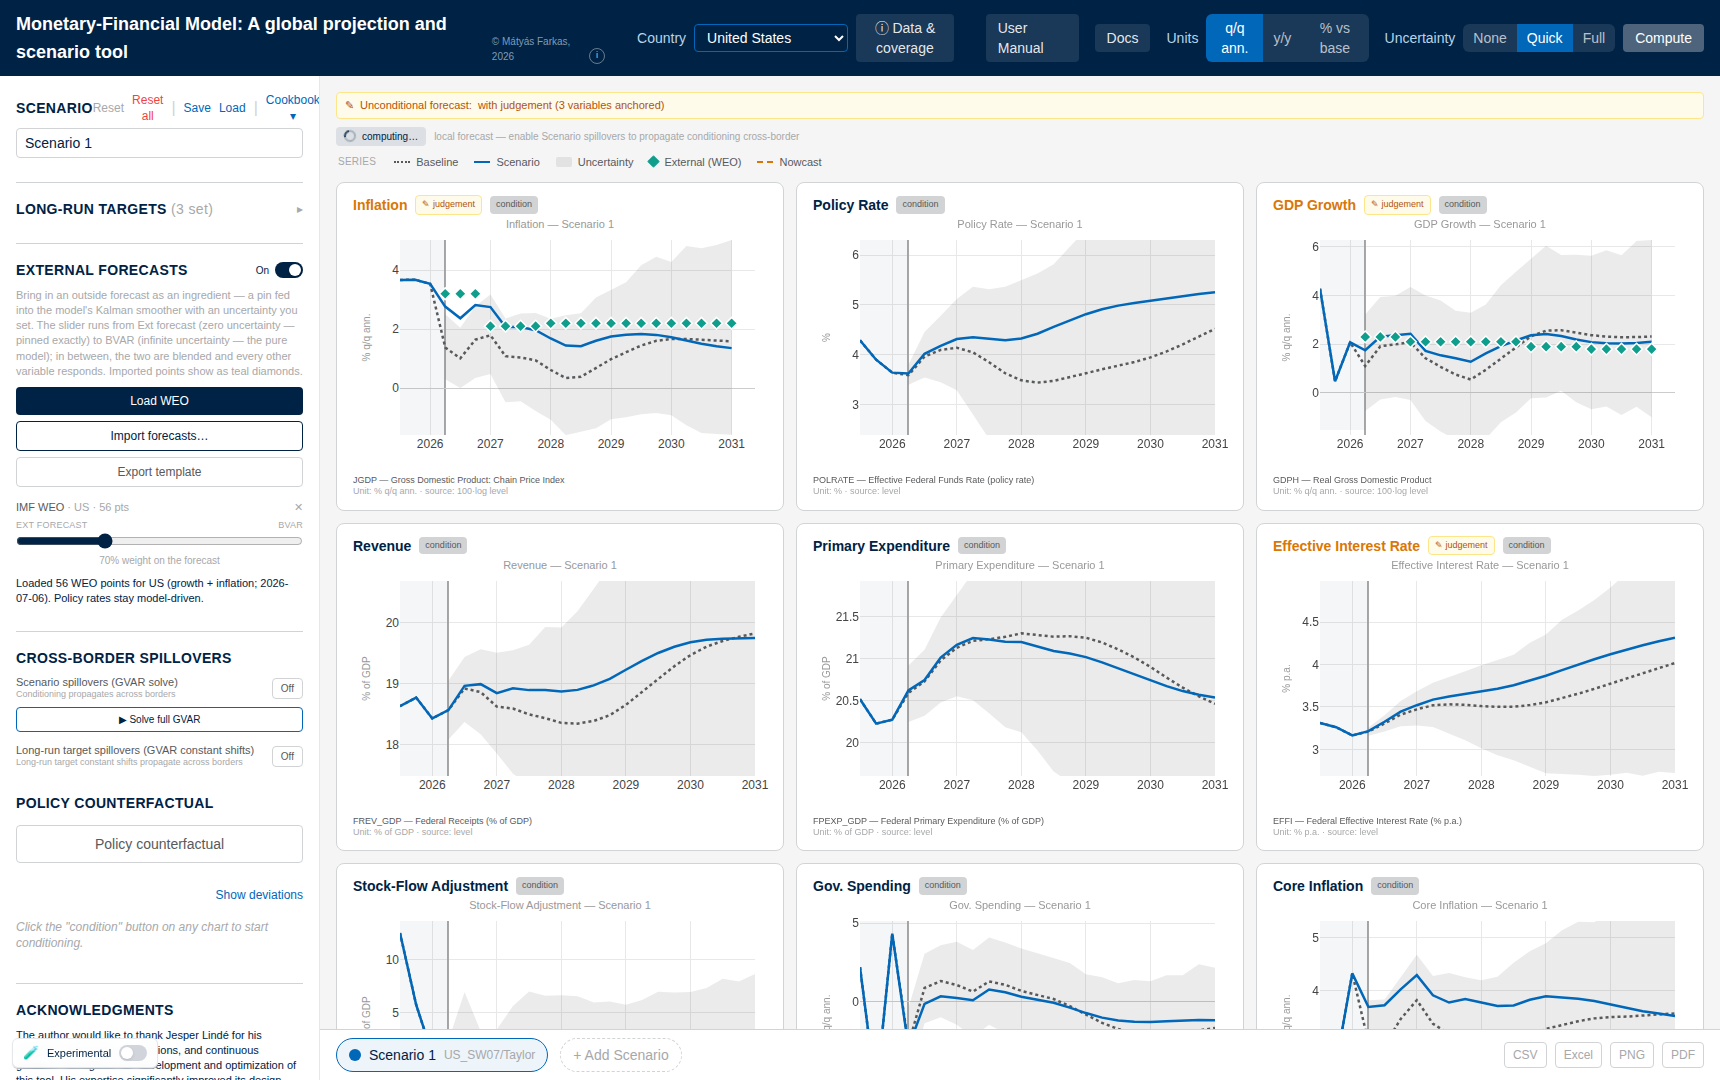
\includegraphics[width=\textwidth]{manual_figs/ui_external_weo.png}
\caption{An outside forecast as an ingredient (\textsf{Load WEO}). The teal diamonds are the imported
WEO growth and inflation points; the trust dial (left rail, here at $70\%$ weight on the
forecast) maps to the measurement-error variance of Eq.~\eqref{eq:trust}, so the scenario blends
the outside path with the model instead of pinning it; policy rates stay model-driven.}
\label{fig:ui-external}
\end{figure}


An imported outside forecast --- IMF WEO, a consensus survey, desk
numbers --- enters as a \emph{soft} pin: an observation with a
measurement variance set by the user's trust in the source, so the model
reconciles the outside number with everything else rather than being
overridden by it. For a cell of variable $j$ at horizon $h$ held with
trust $\tau \in (0,1)$, the measurement variance
in~\eqref{eq:kfinnov} is
\begin{equation}\label{eq:trust}
  R^{\text{ext}}_{h,j}
  \;=\; \widehat{\Var}_{h,j}\,\frac{1-\tau}{\tau},
  \qquad
  \widehat{\Var}_{h,j}
  = \Bigl(\max\bigl(\tfrac{q_{84}-q_{16}}{2},\,10^{-6}\bigr)\Bigr)^2,
\end{equation}
where $q_{84}-q_{16}$ is the model's own shipped predictive band
of~\eqref{eq:bands} at that cell --- so the dial needs no units:
$\tau = \tfrac12$ makes the outside number exactly as informative as
the model's own predictive density, $\tau \ge 0.999$ collapses to the
hard pin~\eqref{eq:R}, and $\tau \to 0$ is a no-op ($\tau$ is clamped to
$[0.001, 0.999]$; the default is $0.7$). Display-unit values are
converted to level-space pins by the conventions of
Section~\ref{sec:delta} (growth targets cumulate; any active long-run
drift of Section~\ref{sec:longrun} is netted out first, so the
\emph{displayed} line lands on the imported number). A cell the user has
pinned by hand always wins over an imported one
(\texttt{externalForecast.ts}).

In the interface (\ui{External forecasts}, left panel): \ui{Load WEO}
imports the IMF World Economic Outlook real-GDP-growth and inflation
forecast for the viewed economy, each annual figure applied softly to
its four quarters; \ui{Export template} writes an Excel file pre-filled
with the model baseline, to be overwritten and re-imported;
\ui{Import forecasts\dots} accepts that file or a small JSON. Each
source appears with its trust slider; imported points draw as teal
diamonds with an error bar that grows as trust falls; the source's
\texttimes{} (or zero trust) removes it. \ui{Export session}/\ui{Import
session} bundle all countries' conditioning, targets, and imports into
one JSON for hand-over. On a coupled economy an imported forecast also
propagates cross-border, with one performance caveat documented in
Section~\ref{sec:gvarsoft}.

\subsection{Scenario uncertainty bands}\label{sec:scenbands}

Pressing \ui{Compute} with \ui{Quick} or \ui{Full} selected draws
$N_b = 50$ or $200$ predictive paths and bands the scenario. The default
construction is deliberately simple and fast:
\begin{enumerate}[label=(\roman*)]
  \item for each band draw, sample a posterior draw
    $(\hat\beta^{(d)}, \hat\Sigma^{(d)})$ from the $D=500$ shipped draws
    (with replacement) and iterate the companion forward from the last
    observed state \emph{with} innovation shocks
    $\eta_h \sim \mathcal{N}(0, \hat\Sigma^{(d)})$ --- a full predictive
    draw carrying both parameter and shock uncertainty;
  \item convert to display units and shift the whole path by the
    (draw-invariant) mean scenario delta of~\eqref{eq:delta};
  \item report the empirical 16th and 84th percentiles per cell.
\end{enumerate}
The band is therefore the model's own predictive range \emph{re-centred
on the scenario path} --- directly comparable to the baseline fan ---
and at the actively pinned quarters of a conditioned variable it is
collapsed onto the line, since an imposed value carries no uncertainty.
On the \ui{\% vs base} impact view the shading instead uses the smoothed
conditional standard deviation from~\eqref{eq:Nrec}: it pinches at hard
pins, shrinks partially at soft pins in proportion
to~\eqref{eq:trust}, and tapers \emph{into} a future pin --- the honest
conditional-variance picture.

\begin{remark}[Why the default band is not the per-draw conditional cloud]\label{rem:bandchoice}
Re-solving the conditional forecast draw by draw produces a genuinely
conditional cloud, but with only a point or two pinned it collapses far
too tightly under the estimated prior --- a band the user reads as
false confidence. The default recentring preserves the full predictive
width; the per-draw conditional construction is available for coupled
economies as the \ui{Experimental} switch (bottom-left), which re-solves
the entire cross-country system per draw
(Section~\ref{sec:gvarbands}). Toggling it clears any band on screen,
because bands built the two ways must not be read against each other.
\end{remark}

\begin{remark}[Long-run targets translate bands rigidly]\label{rem:bandrigid}
A long-run anchor (Section~\ref{sec:longrun}) shifts the central path
and every band quantile by the same deterministic amount, instantly and
without recomputation --- band \emph{widths} are invariant by
construction. Only pins change conditional uncertainty; targets move
where the forecast is headed, not how well it is known.
\end{remark}

%% ================================================================
\section{The global model}\label{sec:gvar}
%% ================================================================

Thirty-three of the deployed economies are coupled into a global VAR
(GVAR) in the tradition of \citet{PesaranSchuermannWeiner2004} and
\citet{DeesDiMauroPesaranSmith2007}: the United States, the euro area as
a single aggregate bloc, and thirty-one further economies, spanning
roughly ninety percent of world GDP (the roster is in
Appendix~\ref{app:tables}). Two design choices organize everything in
this section. First, \emph{coupling is imposed at solve time, not at
estimation time}: each bloc is an independently estimated BVAR, and
cross-country spillovers enter only through the scenario
\emph{deviation}, which propagates as a linear fixed point. Second, the
United States is \emph{fully endogenous}: it carries its own
trade-weighted foreign variables and iterates inside the fixed point
like every other bloc, so shocks abroad feed back into the US --- the
channel a classical frozen dominant unit cannot represent.

The euro area enters as one aggregate by necessity: a fully
disaggregated euro GVAR is non-stationary (the coupling operator's
spectral radius exceeds one, $\rho \approx 1.089$, in the disaggregated
experiment), while aggregation restores contraction. The seventeen
euro-area member states are therefore \emph{standalone} models outside
the coupled system, connected to it through a separate euro-area doorway
(Section~\ref{sec:eamembers}).

\subsection{Star variables and trade weights}\label{sec:stars}

\begin{figure}[!ht]
\centering
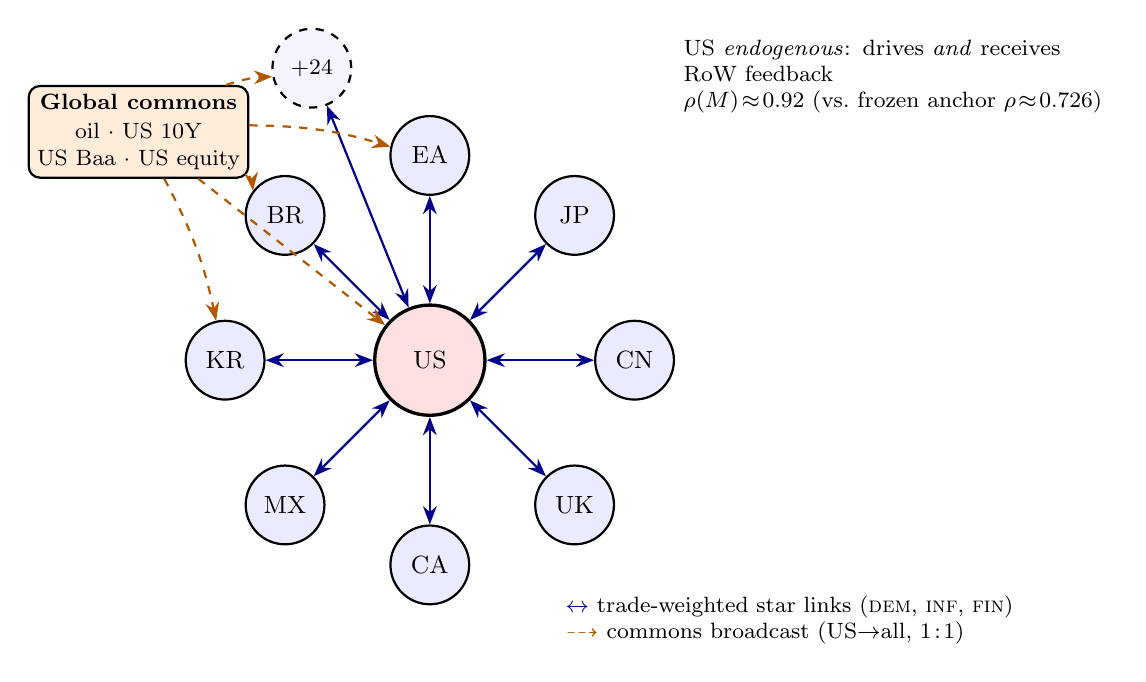
\begin{tikzpicture}[
  >=Stealth,
  font=\small,
  bloc/.style={circle, draw, thick, minimum size=10mm, inner sep=1pt, fill=blue!8},
  hub/.style={circle, draw, very thick, minimum size=14mm, inner sep=1pt, fill=red!12},
  commons/.style={rectangle, rounded corners, draw, thick, fill=orange!15,
                  align=center, inner sep=3pt, font=\footnotesize},
  star/.style={<->, thick, blue!55!black},
  bcast/.style={->, thick, orange!70!black, dashed},
]

% Central dominant US bloc (endogenous)
\node[hub] (US) at (0,0) {US};

% Ring of representative partner blocs (label ~8, indicate "+ 24 more")
\node[bloc] (EA)   at ( 90:2.6) {EA};
\node[bloc] (JP)   at ( 45:2.6) {JP};
\node[bloc] (CN)   at (  0:2.6) {CN};
\node[bloc] (UK)   at (-45:2.6) {UK};
\node[bloc] (CA)   at (-90:2.6) {CA};
\node[bloc] (MX)   at (-135:2.6) {MX};
\node[bloc] (KR)   at (180:2.6) {KR};
\node[bloc] (BR)   at (135:2.6) {BR};

% "+ 24 more" partner blocs
\node[bloc, fill=blue!4, dashed] (more) at (112:4.0) {\footnotesize $+24$};

% Bidirectional trade-weighted star links (US <-> each partner)
\foreach \c in {EA,JP,CN,UK,CA,MX,KR,BR} {\draw[star] (US) -- (\c);}
\draw[star] (US) -- (more);

% Global commons node broadcasting one-directionally to all blocs
\node[commons] (GC) at (-3.7,2.9)
  {\textbf{Global commons}\\[1pt]
   oil $\cdot$ US 10Y\\ US Baa $\cdot$ US equity};
\draw[bcast] (GC) -- (US);
\foreach \c in {EA,BR,KR,more} {\draw[bcast] (GC) to[bend left=8] (\c);}

% Legend / annotations
\node[align=left, font=\footnotesize, anchor=west, text width=6.0cm] at (1.6,-3.3)
  {\textcolor{blue!55!black}{$\leftrightarrow$}\ trade-weighted star links
     (\textsc{dem}, \textsc{inf}, \textsc{fin})\\
   \textcolor{orange!70!black}{$\dashrightarrow$}\ commons broadcast (US$\to$all, $1\!:\!1$)};
\node[align=left, font=\footnotesize, anchor=west, text width=5.4cm] at (3.1,3.6)
  {US \emph{endogenous}: drives \emph{and} receives RoW feedback\\
   $\rho(M)\!\approx\!0.92$ (vs.\ frozen anchor $\rho\!\approx\!0.726$)};

\end{tikzpicture}
\caption{GVAR bloc topology. A central, dominant United States bloc is coupled to
a ring of $32$ Rest-of-World partner blocs (eight labelled---EA, JP, UK, CA, CN,
MX, KR, BR---plus $24$ further blocs) through \emph{bidirectional},
trade-weighted ``RoW star'' links carrying foreign demand (\textsc{dem}),
inflation (\textsc{inf}), and the short rate (\textsc{fin}). A small global-commons
node (oil, the long US rate, US corporate credit, US equity) broadcasts
\emph{one-directionally} and identically ($1\!:\!1$) to every bloc. The US is now a
\emph{fully endogenous} coupled bloc rather than the classical frozen anchor: it
feeds the rest of the world \emph{and} receives feedback, raising the coupling
operator's spectral radius from $\rho(M)\approx0.726$ (frozen-US, RoW-only) to
$\rho(M)\approx0.92$ at the full $33$-bloc endogenous-US configuration (the value
stored in the shipped \texttt{coupling\_default.json.gz}; it moves slightly with
each refit), both contractive so the fixed point $x = Mx + d$ is well defined
(Sections~\ref{sec:stars} and~\ref{sec:coupling}).}
\label{fig:gvar-topology}
\end{figure}

Every coupled bloc carries three trade-weighted \emph{star} variables
summarizing its foreign environment, the weak-exogeneity device of the
GVAR literature: foreign demand (\texttt{ROWDEM}), foreign inflation
(\texttt{ROWINF}), and foreign financial conditions (\texttt{ROWFIN}).
At estimation time the stars are built as levels from the partners'
\emph{completed} panels (Section~\ref{sec:gvarem}): with $w_{cj}$ the
trade weight of partner $j$ in receiver $c$ and $\ell_{j,t}$ the
partner's stored $100\ln$ level,
\begin{equation}\label{eq:star}
  \text{ROWDEM}_{c,t}
  = 4 \sum_{j} \tilde{w}_{cj}\,
      \bigl(\ell^{\,\text{gdp}}_{j,t} - \ell^{\,\text{gdp}}_{j,t-1}\bigr),
  \qquad
  \text{ROWFIN}_{c,t} = \sum_{j} \tilde{w}_{cj}\, r_{j,t},
\end{equation}
(\texttt{ROWINF} as \texttt{ROWDEM} on price levels) --- annualized
growth for the two macro stars, the factor $4$
of~\eqref{eq:growth}, and a level average of partner short rates
$r_{j,t}$ for the financial star. The weights $\tilde{w}_{cj}$ are
renormalized \emph{per component and per quarter} over the partners
actually present and eligible, so absent or excluded mass is reabsorbed
rather than dropped: rate-less blocs (Switzerland, Norway) leave their
partners' \texttt{ROWFIN}; Argentina's hyperinflation episode is
excluded from partners' \texttt{ROWINF} and \texttt{ROWFIN} while its
real demand stays in \texttt{ROWDEM}. (A deflate-by-subtraction rule
exists for blocs reporting nominal GDP; since China was re-sourced to a
real chain-linked volume index in the June-2026 re-estimate, the set of
such blocs is currently empty.)

The bilateral weights come from the IMF's International Merchandise
Trade Statistics (exports plus imports, 2021--2023 average, euro area
as a single counterpart) and ship as one row per coupled bloc --- the
US row included --- each summing to one with a zero diagonal
(\texttt{weights\_24bloc.json}; the file name is historical, the file
lists all 33 blocs). The topology is \emph{not} hardcoded: a bloc is a
coupled member if and only if its specification carries the three
\texttt{row}-tagged stars \emph{and} it has a weights row, and the US is
treated as endogenous if and only if its own model satisfies the same
test. Absent either, the engine falls back to the legacy frozen-anchor
solve unchanged.

\paragraph{Time-varying weights (a gated capability).} The single
fixed-window row above can be replaced, \emph{at estimation time}, by an
annual bilateral panel: when the artifact
\texttt{weights\_timevarying.json} is present (and
\texttt{GVAR\_TV\_WEIGHTS}${\neq}0$), \texttt{buildstars} reads each
quarter's stars off that quarter's calendar-year row, clamped to the
file's span, with a partner absent from a given year assigned weight
zero and reabsorbed by the same per-component, per-quarter
renormalization as above (\texttt{export\_bvar\_gvar24\_loop.m}). The
weights then reach the star \emph{history} on which the blocs are
estimated, rather than freezing the 2021--2023 average across the whole
sample. The staged panel is annual IMTS bilateral trade for
$1995$--$2024$ over $39$ blocs. The empirical picture it carries is not
the textbook monotone story: the US-to-China trade share rises to a
$2017$ peak ($0.176$) and then \emph{falls} after the 2018 tariff
episode (to $0.119$ by $2024$), while the US-to-euro-area share does
\emph{not} decline but drifts up to $0.178$. This remains a gated
capability: absent the artifact (or with \texttt{GVAR\_TV\_WEIGHTS}${=}0$)
the static row is used everywhere, byte-identical to the shipped models,
and the solve-time coupling of Section~\ref{sec:coupling} still reads the
single current-year row --- promoting the time-varying panel to the
live solver is a separate step.

\subsection{Estimation: an EM fixed point in the completed stars}\label{sec:gvarem}

Before the formal statement, here is the idea in plain terms. To estimate
any one country's model you need its \emph{foreign environment} --- what
its trading partners' demand, inflation, and interest rates are doing. But
each partner's path is itself the output of that partner's model, which
needs \emph{its} foreign environment, and so on around the world:
everything depends on everything, so no country can be estimated on its
own and first. The way out is to treat the unknown foreign environment as
\emph{missing data} and fill it in by iterating. Start from a rough guess
of the foreign environment for every country; estimate each country's
model against its guess (filling in the pandemic holes in the same step);
then read off from the freshly-estimated countries what the foreign
environment \emph{actually} turned out to be, and re-estimate against
that. Repeat. Each pass the guesses become more mutually consistent, and
the loop stops when the environment each country \emph{assumed} matches
the one its partners \emph{produce} --- when the guesses have come true.
That self-consistent set of country models is the estimate.

A concrete image helps: fifty country desks share one room, each
forecasting its own economy but needing its neighbours' forecasts as
inputs. Everyone pencils in a rough guess for the neighbours and produces
a first forecast; the forecasts are passed back around the room and each
desk redoes its own with the updated inputs; the numbers keep circulating
until nobody's change any more. This is exactly the
expectation--maximization logic of \citet{DempsterLairdRubin1977} with the
``rest of the world'' --- and the pandemic gaps --- as the missing data:
an \textbf{E-step} that fills in the blanks given the current models, and
an \textbf{M-step} that re-fits the models given the filled-in blanks,
iterated to a fixed point. Two things are worth keeping straight. Nothing
is accepted or rejected \emph{across} countries: coherence is the loop's
stopping rule, not an acceptance test, and the loop settles on one
consistent set of paths rather than a distribution of draws. The genuine
Bayesian sampling --- the simulation smoother that draws the missing cells
and the Metropolis step that updates the shrinkage hyperparameters ---
lives \emph{inside} each country's single fit (Section~\ref{sec:covid}),
one level below the loop.

\begin{figure}[!ht]
\centering
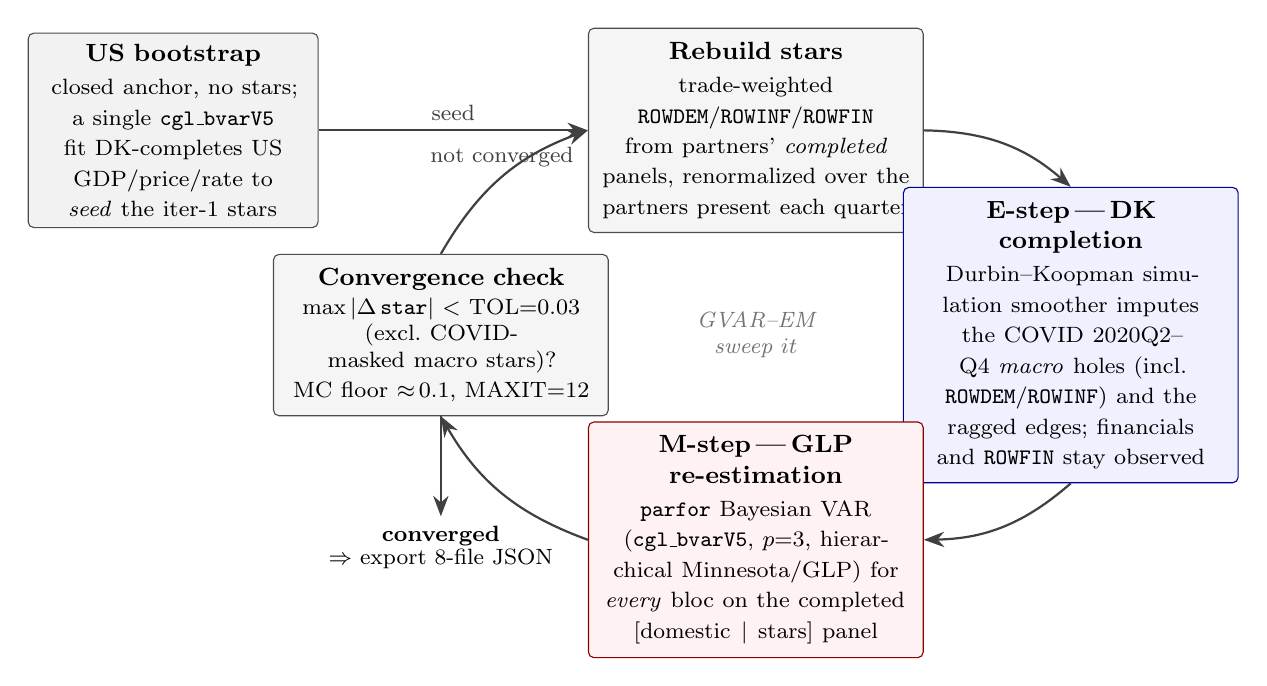
\begin{tikzpicture}[
    >={Stealth[length=2.6mm]},
    font=\small,
    boot/.style={rounded corners=2pt, draw=black!70, fill=black!5,
                 align=center, inner sep=4pt, text width=3.4cm},
    estep/.style={rounded corners=2pt, draw=blue!60!black, fill=blue!6,
                  align=center, inner sep=5pt, text width=3.9cm},
    mstep/.style={rounded corners=2pt, draw=red!55!black, fill=red!5,
                  align=center, inner sep=5pt, text width=3.9cm},
    starbox/.style={rounded corners=2pt, draw=black!70, fill=black!4,
                 align=center, inner sep=5pt, text width=3.9cm},
    convbox/.style={rounded corners=2pt, draw=black!70, fill=black!4,
                 align=center, inner sep=5pt, text width=3.9cm},
    flow/.style={->, thick, black!75},
]
% --- US bootstrap: entry into the loop (seeds the first stars) ---
\node[boot] (boot) at (-7.4,2.6)
  {\textbf{US bootstrap}\\[1pt]
   \footnotesize closed anchor, no stars; a single
   \texttt{cgl\_bvarV5} fit DK-completes US GDP/price/rate to
   \emph{seed} the iter-1 stars};

% --- cycle nodes (clockwise: stars -> E -> M -> conv -> stars) ---
\node[starbox] (stars) at (0,2.6)
  {\textbf{Rebuild stars}\\[1pt]
   \footnotesize trade-weighted \texttt{ROWDEM}/\texttt{ROWINF}/%
   \texttt{ROWFIN} from partners' \emph{completed} panels,
   renormalized over the partners present each quarter};

\node[estep] (estep) at (4.0,0)
  {\textbf{E-step\,---\,DK completion}\\[1pt]
   \footnotesize Durbin--Koopman simulation smoother imputes the
   COVID 2020Q2--Q4 \emph{macro} holes (incl.\ \texttt{ROWDEM}/%
   \texttt{ROWINF}) and the ragged edges; financials and
   \texttt{ROWFIN} stay observed};

\node[mstep] (mstep) at (0,-2.6)
  {\textbf{M-step\,---\,GLP re-estimation}\\[1pt]
   \footnotesize \texttt{parfor} Bayesian VAR (\texttt{cgl\_bvarV5},
   $p{=}3$, hierarchical Minnesota/GLP) for \emph{every} bloc on the
   completed $[\text{domestic}\mid\text{stars}]$ panel};

\node[convbox] (conv) at (-4.0,0)
  {\textbf{Convergence check}\\[1pt]
   \footnotesize $\max|\Delta\,\texttt{star}| < \mathrm{TOL}{=}0.03$
   (excl.\ COVID-masked macro stars)?\\
   MC floor ${\approx}\,0.1$, $\mathrm{MAXIT}{=}12$};

% --- entry arrow ---
\draw[flow] (boot.east) -- node[above,font=\footnotesize]{seed} (stars.west);

% --- the clockwise cycle ---
\draw[flow] (stars.east)  to[bend left=20] (estep.north);
\draw[flow] (estep.south) to[bend left=20] (mstep.east);
\draw[flow] (mstep.west)  to[bend left=20] (conv.south);
\draw[flow] (conv.north)  to[bend left=20]
  node[above,font=\footnotesize]{not converged} (stars.west);

% --- converged exit ---
\node[align=center, font=\footnotesize] (out) at (-4.0,-2.7)
  {\textbf{converged}\\[-1pt]$\Rightarrow$ export 8-file JSON};
\draw[flow] (conv.south) -- (out.north);

% --- loop label ---
\node[font=\footnotesize\itshape, text=black!55, align=center] at (0,0)
  {GVAR--EM\\sweep $it$};
\end{tikzpicture}
\caption{The GVAR-EM estimation loop under pervasive missingness
\citep{GiannoneLenzaPrimiceri2019, DurbinKoopman2002}. A closed US
bootstrap (no stars) is estimated once to seed the first trade-weighted
foreign variables. Each sweep then (i)~rebuilds the
\texttt{ROWDEM}/\texttt{ROWINF}/\texttt{ROWFIN} stars from partners'
completed panels, renormalized over the partners present each quarter,
and (ii)~re-estimates every bloc by hierarchical-prior Bayesian VAR
(Gibbs, run in \texttt{parfor}). Within each bloc's single
\texttt{cgl\_bvarV5} pass the \textbf{E-step}---a Durbin--Koopman
simulation-smoother completion that imputes the COVID macro holes (the
fixed 2020Q2--Q4 window, with financial series and \texttt{ROWFIN} held
observed) and the ragged, unbalanced-panel edges---and the
\textbf{M-step}---the posterior re-estimation of the VAR coefficients on
the completed $[\text{domestic}\mid\text{stars}]$ panel---are carried out
jointly by the same sampler. The sweep repeats until the foreign
components stop moving, $\max|\Delta\,\texttt{star}| < \mathrm{TOL}=0.03$
(evaluated after the second sweep and excluding the COVID-masked macro
stars, whose cross-iteration churn is Monte-Carlo noise with floor
${\approx}\,0.1$), capped at $\mathrm{MAXIT}=12$ iterations.}
\label{fig:em-loop}
\end{figure}

The stars cannot be built directly from observed data: the panels are
unbalanced (blocs enter the sample at different dates), the pandemic
macro cells are deliberately missing (Section~\ref{sec:covid}), and
several financial series start late. A star built only on complete
quarters would truncate the sample to the common balanced span ---
exactly the information loss the data-augmentation design avoids. The
estimator therefore iterates completion and re-estimation to a fixed
point in the stars \citep[in the spirit of][]{DempsterLairdRubin1977}:
\begin{itemize}
  \item \textbf{E-step (completion).} For each bloc, one call to the
    data-augmentation sampler of Section~\ref{sec:covid} on the panel
    $[\,\text{domestic} \mid \text{stars}\,]$ imputes every missing cell
    (COVID macro mask included) by the Durbin--Koopman simulation
    smoother; the posterior-mean completed panel is retained.
  \item \textbf{M-step (re-estimation).} The same call re-estimates the
    bloc's coefficients under the GLP prior on the completed data; the
    posterior means $(\hat\beta_c, \hat\Sigma_c)$ and the thinned draws
    are what ships.
  \item \textbf{Outer loop.} All blocs' stars are rebuilt
    via~\eqref{eq:star} from the \emph{frozen} start-of-sweep
    completions, the blocs are re-estimated in parallel (a Jacobi sweep,
    order-independent), and the loop repeats until the stars stop
    moving:
    $\max_c \|x^{*(m)}_c - x^{*(m-1)}_c\|_\infty < \textsc{tol} = 0.03$
    (COVID-masked macro-star cells excluded from the metric --- their
    cross-iteration churn is imputation Monte-Carlo noise, with an
    observed floor near $0.13$, so convergence in practice is a plateau
    at the noise floor), capped at $\textsc{maxit} = 12$ sweeps. A
    one-shot, no-stars US completion seeds the first sweep.
\end{itemize}
Algorithm~\ref{alg:emgvar} states the loop
(\texttt{pipeline/export\_bvar\_gvar24\_loop.m}). Setting
$\textsc{maxit}=1$ recovers the single-pass mode used for the standalone
blocs, whose stars are read off data once. Relative to the classical
fixed-weight GVAR --- stars built once from observed data on a balanced
panel, one OLS pass per country --- every departure here serves the
unbalanced panel: model-based completion flowing \emph{into} the stars,
per-quarter renormalized weights, Bayesian shrinkage with the
COVID-as-missing treatment, and the star fixed point itself. The
out-of-sample evaluation of Section~\ref{sec:eval} races exactly this
apparatus against its classical ancestor.

\begin{algorithm}[!ht]
\caption{GVAR-EM estimation loop
(\texttt{export\_bvar\_gvar24\_loop.m}).}
\label{alg:emgvar}
\algIn{per-bloc observed panels with \texttt{NaN} holes; trade weights;
eligibility rules; $\textsc{tol}=0.03$, $\textsc{maxit}=12$; fixed COVID
window 2020Q2--Q4.}
\algOut{per-bloc posterior means and draws; converged stars; the
eight-file export.}
\begin{algsteps}
\item \algComment{Bootstrap.} Complete the US panel with no stars
  (COVID macro cells masked); its posterior-mean completion seeds the
  first-sweep stars. Under \textsc{us\_endogenous} the US then joins the
  swept set with its own \texttt{ROW*\_US} stars.
\item \algKw{for} $m = 1, \dots, \textsc{maxit}$:
\item \algInd rebuild every receiver's stars~\eqref{eq:star} from the
  frozen start-of-sweep completed panels;
\item \algInd \algKw{parfor each} bloc $c$: mask the COVID macro cells
  (domestic macro columns $+$ \texttt{ROWDEM}, \texttt{ROWINF};
  financials and \texttt{ROWFIN} stay observed); one
  \texttt{cgl\_bvarV5} call $\Rightarrow$ completed panel
  $+$ $(\hat\beta_c, \hat\Sigma_c)$ $+$ draws;
\item \algInd commit the new completions;
  $\mathrm{mc} \gets \max_c\|\Delta x^{*}_c\|_\infty$ (COVID macro-star
  cells excluded);
\item \algInd \algKw{if} $m > 1$ \algKw{and}
  $\mathrm{mc} < \textsc{tol}$: \algKw{break}.
\item Export each bloc to the eight-file JSON contract.
\end{algsteps}
\end{algorithm}

\paragraph{A two-stage E-step.} The imputation inside each M-step
(Section~\ref{sec:covid}) can be run in either of two ways, and the loop
uses both in sequence. During the outer sweeps the Durbin--Koopman
completion is carried out with a \emph{fixed companion}: the smoother's
state-space matrices are built once from the posterior-mode fit and held
across the Gibbs draws (\texttt{fixedcomp}$=1$ in
\texttt{estimate\_bloc}, \texttt{export\_bvar\_gvar24\_loop.m}). With the
sampler's random stream reset per call, consecutive sweeps then share
their random numbers, so a bloc's star moves only for \emph{systematic}
reasons and the Jacobi fixed point contracts to \textsc{tol} --- a run
descends, e.g., $14.7 \to 1.07 \to 0.20 \to 0.11$ to a plateau at the
Monte-Carlo floor. The textbook alternative rebuilds the companion from
the current $(\beta,\Sigma)$ draw at every Gibbs sweep --- exact
Tanner--Wong data augmentation (\texttt{cgl\_bvarV5.m};
\texttt{CGL\_FIXED\_COMPANION}${=}0$) --- but re-randomizing the
completions each sweep breaks the common-random-number coupling, leaving
a star-churn floor that never meets \textsc{tol}. The coupled estimator
therefore uses the fixed-companion sweeps throughout, and \emph{ships the
fixed-companion posterior} from the converged outer loop. An optional
exact-data-augmentation \emph{polish} pass at the frozen stars is available
(\texttt{GVAR\_POLISH\_EXACT}${=}1$) but is \emph{off by default for the
coupled system}: exact augmentation marginally raises companion persistence
and lifts the coupled operator's spectral radius above one
(\S\ref{sec:coupling}), so it would leave pinned-scenario spillovers
non-contractive. Standalone single-bloc estimators (the euro members) run
exact data augmentation directly, having no outer loop --- and no coupled
operator --- to keep contractive.

\subsection{Solve-time coupling: a linear fixed point}\label{sec:coupling}

\begin{figure}[!ht]
  \centering
  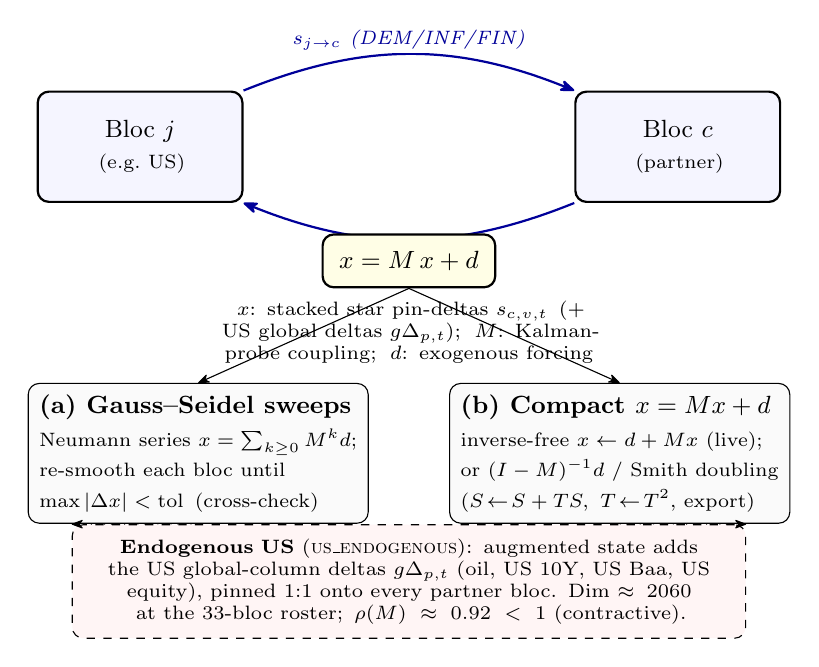
\begin{tikzpicture}[
    >={Stealth[round]},
    font=\small,
    bloc/.style={draw, rounded corners, minimum width=26mm, minimum height=14mm,
                 align=center, thick, fill=blue!4},
    route/.style={draw, rounded corners, minimum width=42mm, align=left,
                  inner sep=4pt, fill=black!2},
    star/.style={font=\scriptsize\itshape, fill=white, inner sep=1pt},
  ]
    % --- two coupled blocs (the cycle) ---
    \node[bloc] (j) {Bloc $j$\\\scriptsize\,(e.g.\ US)};
    \node[bloc, right=42mm of j] (c) {Bloc $c$\\\scriptsize\,(partner)};

    % star-pin feedback cycle j <-> c
    \draw[->, thick, blue!60!black] (j.north east) to[bend left=22]
      node[star, above] {$s_{j\to c}$ (DEM/INF/FIN)} (c.north west);
    \draw[->, thick, blue!60!black] (c.south west) to[bend left=22]
      node[star, below] {$s_{c\to j}$} (j.south east);

    % --- fixed-point equation ---
    \coordinate (jc) at ($(j)!0.5!(c)$);
    \node[below=11mm of jc, draw, rounded corners, thick,
          fill=yellow!10, inner sep=6pt] (eq)
      {$\displaystyle x = M\,x + d$};
    \node[below=1pt of eq, font=\scriptsize, align=center, text width=58mm]
      {$x$: stacked star pin-deltas $s_{c,v,t}$ \,(+ US global deltas $g\Delta_{p,t}$);
       \;$M$: Kalman-probe coupling; \;$d$: exogenous forcing};

    % --- two solution routes ---
    \node[route, below left=12mm and -6mm of eq] (gs)
      {\textbf{(a) Gauss--Seidel sweeps}\\[1pt]
       \scriptsize Neumann series $x=\sum_{k\ge0}M^{k}d$;\\
       \scriptsize re-smooth each bloc until\\
       \scriptsize $\max|\Delta x|<\text{tol}$\, (cross-check)};
    \node[route, below right=12mm and -6mm of eq] (dir)
      {\textbf{(b) Compact $x = M x + d$}\\[1pt]
       \scriptsize inverse-free $x\leftarrow d+Mx$ (live);\\
       \scriptsize or $(I-M)^{-1}d$ / Smith doubling\\
       \scriptsize ($S\!\leftarrow\!S+TS,\ T\!\leftarrow\!T^{2}$, export)};
    \draw[->] (eq.south) -- (gs.north);
    \draw[->] (eq.south) -- (dir.north);

    % --- endogenous-US annotation ---
    \coordinate (gsdir) at ($(gs)!0.5!(dir)$);
    \node[draw, dashed, rounded corners, below=9mm of gsdir,
          fill=red!4, inner sep=5pt, align=center, text width=82mm, font=\scriptsize] (us)
      {\textbf{Endogenous US} (\textsc{us\_endogenous}): augmented state adds the US
       global-column deltas $g\Delta_{p,t}$ (oil, US 10Y, US Baa, US equity),
       pinned $1{:}1$ onto every partner bloc.
       Dim $\approx 2060$ at the $33$-bloc roster; \,$\rho(M)\approx 0.92<1$ (contractive).};
    \draw[->, dotted] (gs.south) -- (us.north west);
    \draw[->, dotted] (dir.south) -- (us.north east);
  \end{tikzpicture}
  \caption{Solve-time cross-country coupling as the affine fixed point
    $x = M\,x + d$. Two coupled blocs exchange trade-weighted star pin-deltas
    (DEM/INF/FIN), forming the feedback cycle; the deviation state $x$ stacks
    these pins (plus the US global-column deltas under an endogenous US). The
    fixed point admits two equivalent solutions---(a) Gauss--Seidel/Neumann
    sweeps through the Durbin--Koopman smoother, used as the cross-check, and (b)
    the compact $M$-state recursion, solved inverse-free by the Neumann
    fixed-point $x\leftarrow d+Mx$ on the production path (the explicit
    $(I-M)^{-1}d$ / Smith doubling are reserved for the small frozen-anchor case
    and the export-time precompute, since the in-browser $O(\dim^{3})$ inverse is
    prohibitive at $\dim\approx 2060$). With the US endogenous the augmented
    state has dimension $\approx 2060$ and spectral radius
    $\rho(M)\approx 0.92<1$, so the iteration contracts and the two routes agree
    to $\sim 10^{-9}$.}
  \label{fig:coupling}
\end{figure}

At solve time the coefficients are frozen, and the key observation is
that the conditional-forecast operator of Section~\ref{sec:cond} is
\emph{affine in the pinned values for a fixed pin pattern}: the filter
and smoother are linear in the data. Each bloc's level forecast can
therefore be written
\begin{equation}\label{eq:kernels}
  x_c \;=\; a_c \;+\; \sum_{v}\sum_{s=0}^{H-1} K_c[v][s]\; \Delta^{*}_{c,v,s},
\end{equation}
where $a_c$ is the bloc's forecast with its \emph{own} pins active and
its stars and global columns held at baseline, $\Delta^{*}_{c,v,s}$ is
the deviation pinned on star (or global) column $v$ at horizon $s$, and
the kernel $K_c[v][s] \in \R^{H\times n}$ is the smoothed response to a
unit bump of that single cell. The kernels are computed from one
filter--smoother pass per bloc by value-independent delta recursions
(\texttt{affineBlocKernels}, numerically identical to explicit probing
to below $10^{-9}$ and an order of magnitude faster), and they depend
only on the bloc's coefficients and its own-pin \emph{pattern} --- never
on pin values or on partners --- so they are cached and reused across
every value change of an interactive drag.

The solver never rebuilds star \emph{levels} from partner levels.
It pins each receiver's star column at its own baseline plus the
trade-weighted partner \emph{deviation}:
\begin{equation}\label{eq:stardelta}
  \Delta^{*}_{c,\textsc{dem},t}
  = \sum_{j}\tilde{w}_{cj}\cdot 4\,
    \Bigl[\bigl(x^{\text{scen}}_{j,t}-x^{\text{scen}}_{j,t-1}\bigr)
        - \bigl(x^{\text{base}}_{j,t}-x^{\text{base}}_{j,t-1}\bigr)\Bigr],
  \qquad
  \Delta^{*}_{c,\textsc{fin},t}
  = \sum_{j}\tilde{w}_{cj}\,
    \bigl(r^{\text{scen}}_{j,t}-r^{\text{base}}_{j,t}\bigr),
\end{equation}
read off the partners' gdp/price/rate columns (at $t=0$ the shared last
in-sample level cancels in the difference). Stacking all star deviations
--- and, with the US endogenous, the deviations of the four US-determined
global columns (Section~\ref{sec:commons}) --- into a vector $x$, the
deviation system is the linear fixed point
\begin{equation}\label{eq:fp}
  x = M\,x + d,
\end{equation}
where $d$ collects the exogenous forcing (each bloc's own pins evaluated
at zero partner deviation, plus any long-run drift,
Section~\ref{sec:driftgvar}) and $M$ carries three coupling families:
star $\leftarrow$ partner star (through the kernels and weights,
equations~\eqref{eq:kernels}--\eqref{eq:stardelta}, the US on both
sides), the US-global definition rows (a global column's deviation as
the US's own response to its star pins), and star $\leftarrow$ global (a
partner's star response to its own global pin). At the deployed roster
the state dimension is $33 \times 3 \times 20 + 4 \times 20 = 2060$, and
the shipped operator has spectral radius
\begin{equation}\label{eq:rho}
  \rho(M) = 0.945 \;<\; 1
\end{equation}
(the value stored in the shipped coupling artifact, $0.945494$,
eigendecomposition-exact --- before 2026-07-17 the field read $0.935044$ from an
under-converged power iteration on a complex dominant pair; it moves
with each re-estimate), so the map is contractive, $(I-M)$ is
nonsingular, and the fixed point is unique.

The fixed point is solved three equivalent ways, all implemented in
\texttt{gvarSolve.ts}:
\begin{enumerate}[label=(\alph*)]
  \item \textbf{Gauss--Seidel sweeps}: re-condition each bloc in turn on
    the freshest partner deviations until the maximum level change falls
    below $10^{-4}$ (at most 12 sweeps) --- the term-by-term Neumann sum
    $\sum_k M^k d$, and the reference the other routes are validated
    against;
  \item \textbf{closed form} $x = (I-M)^{-1} d$, using a precomputed
    inverse (below), followed by one conditional-forecast pass per bloc
    to reconstruct all free variables;
  \item \textbf{inverse-free Neumann iteration} $x \leftarrow d + Mx$
    (tolerance $10^{-10}$ relative, capped at 2000 iterations) when the
    precomputed inverse is unusable --- the in-browser $O(\dim^3)$
    inverse at $\dim = 2060$ would take the better part of an hour and
    is never built live.
\end{enumerate}
The routes agree to $10^{-6}$ or better in the validation battery.
Divergence is \emph{detected, not prevented}: if a future roster or
degenerate pin set pushed $\rho(M) \ge 1$, the iterations' convergence
flag trips, a console warning fires, and the result is not cached ---
but a path is still returned (Section~\ref{sec:knownissues}).

\paragraph{The coupling artifact and the model signature.}\label{sec:modelsig}
$M$ depends on the models and the pin \emph{pattern}, not the pin
values, so for the default (empty) pattern both $M$ and $(I-M)^{-1}$ are
precomputed offline --- the inverse by a \textsc{blas} solve in MATLAB
(\texttt{app/scripts/invert\_coupling.m}; a NumPy fallback ships
alongside) --- rounded to six significant figures, gzipped
(\texttt{coupling\_default.json.gz}, about 30\,MB compressed), and
decompressed in the browser at load. Hydrating it reduces the first
complete solve from a cold build of many minutes to a few seconds; it is
mandatory infrastructure, not an optimization. A stale artifact is
refused by a \emph{model signature}: per bloc, the dimensions
$(n_c, p_c, H_c)$ and three six-digit fingerprints of the posterior mean
--- the first equation's intercept $\hat\beta_{0,0}$, the far corner of
the last lag row $\hat\beta_{n_c p_c,\, n_c-1}$ (zero-indexed; recall
the intercept is row zero), and the leading residual variance
$\hat\Sigma_{0,0}$. Any re-estimation flips the signature, and the
solver falls back to route (c). A pin on any coupled bloc changes the
pattern and likewise bypasses the cached inverse; only the changed
bloc's kernels are re-probed.

\subsection{Global commons}\label{sec:commons}

Four US-determined series are carried by every bloc: the WTI oil price
(\texttt{GLB\_OIL}), the US 10-year yield (\texttt{GLB\_USLR}), the US
Baa corporate yield (\texttt{GLB\_USBAA}), and US equity
(\texttt{GLB\_USEQ}). In the US model they are ordinary endogenous
variables; every other bloc carries the same identifiers (matched by
name, never by position) as weakly exogenous columns that the solver
pins \emph{by deviation}:
\begin{equation}\label{eq:globalpin}
  \widehat{\text{GLB}}_{c,t}
  = \bar{\text{GLB}}_{c,t}
  + \bigl(\text{GLB}^{\text{scen}}_{\text{US},t}
        - \bar{\text{GLB}}_{\text{US},t}\bigr),
\end{equation}
each bloc's own baseline plus the US deviation. Pinning the US
\emph{level} instead would inject the blocs' baseline gaps (tens of
$100\ln$ units) as spurious shocks; the deviation convention gives a
zero-scenario no-op exactly and an identical common shock under
conditioning. With the US endogenous the global deviations are unknowns
of~\eqref{eq:fp} --- this is precisely the second and third coupling
family --- so a partner shock that moves the US moves the commons, which
feed back to every other bloc, without double counting. On screen the
commons are conditionable on the US and read-only elsewhere.

\subsection{Operating the global solve}\label{sec:gvarusage}

\begin{figure}[!ht]
\centering
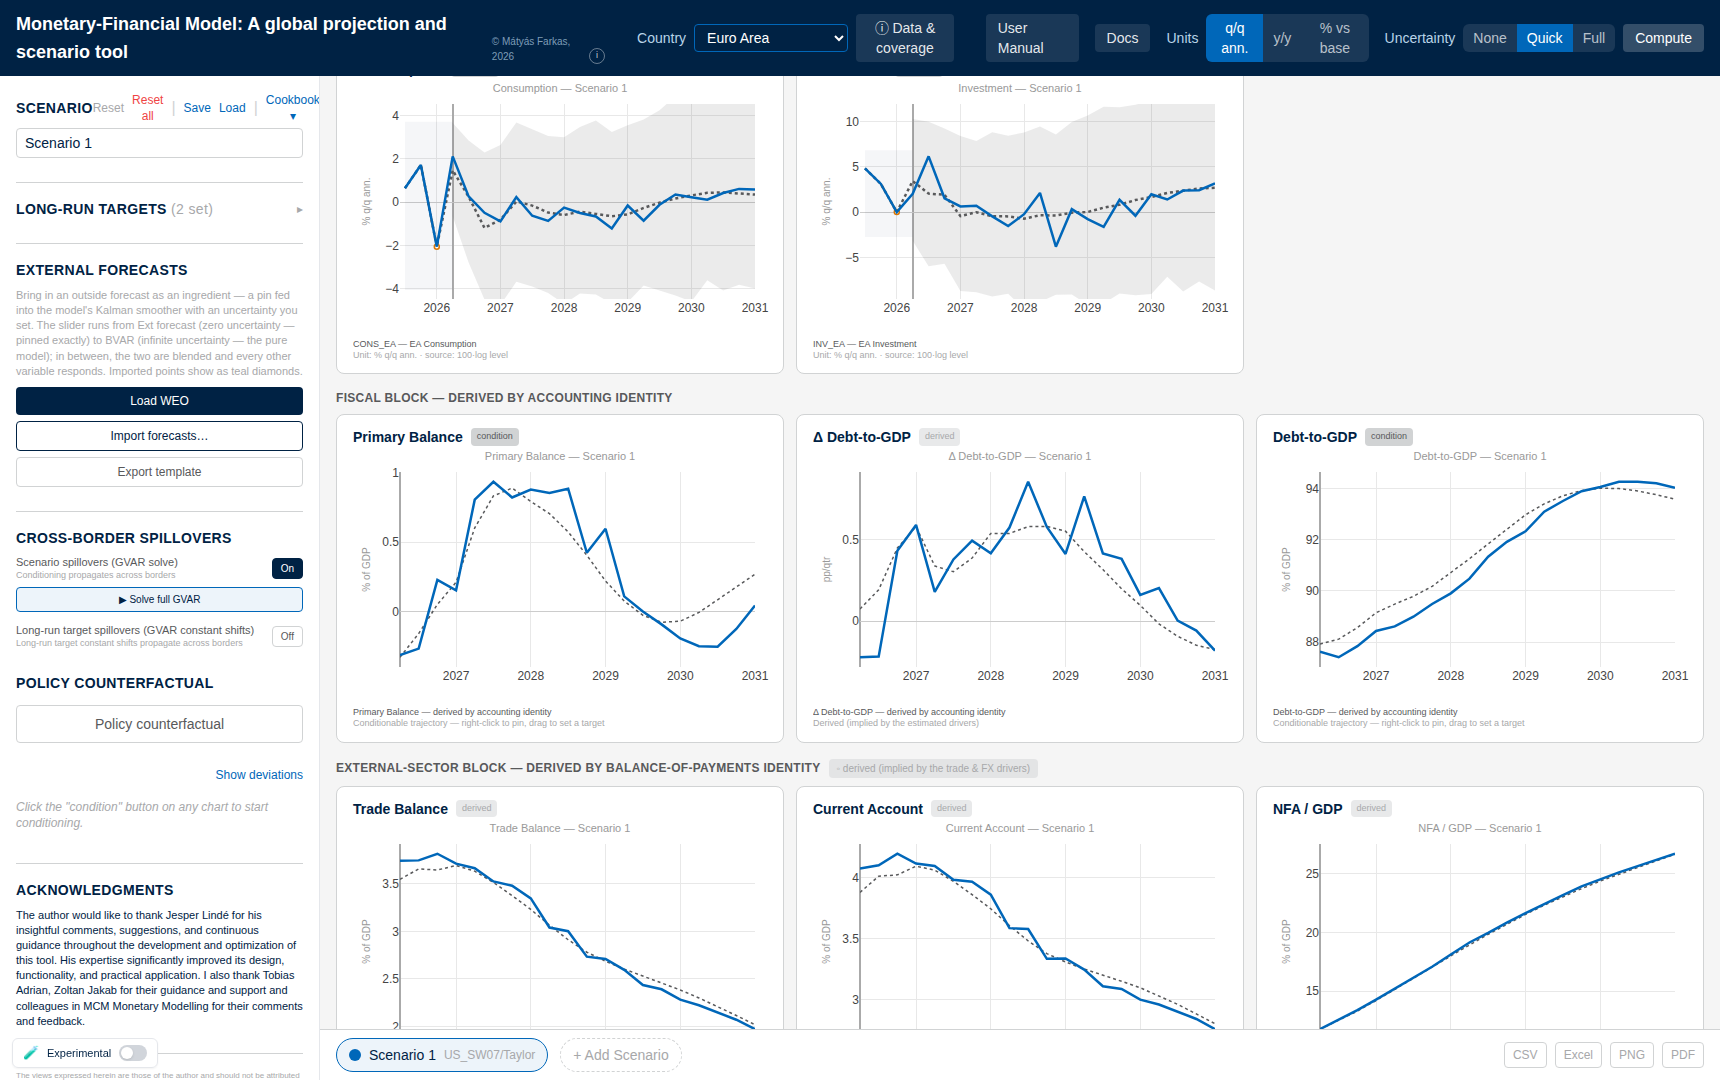
\includegraphics[width=\textwidth]{manual_figs/ui_gvar_ea.png}
\caption{The euro-area view after \textsf{Solve full GVAR} on a US tightening scenario (spillovers
\textsf{On}). The conditioning entered in the United States has propagated cross-border: euro-area
consumption and investment deviate from baseline (dotted), and the derived satellite blocks ---
the fiscal block of \S\ref{sec:fiscal} and the external-sector block of \S\ref{sec:external} ---
re-solve on the coupled paths. Switching countries after a full solve always shows the same
converged system state.}
\label{fig:ui-gvar-ea}
\end{figure}


By default a scenario moves only the economy on screen; partners stay
frozen, and a status line says so. Cross-border transmission is explicit
and two-tier:
\begin{itemize}
  \item \ui{Scenario spillovers (GVAR solve)} (left panel,
    \ui{Cross-border spillovers}) switches on live propagation. While
    editing, the tool shows the \emph{direct preview} --- one
    cross-country hop through the cached kernels, no fixed-point
    feedback, sub-second --- flagged by an amber \ui{GVAR DIRECT
    preview} badge above the grid.
  \item \ui{Solve full GVAR} (or \ui{Compute}) runs the complete fixed
    point~\eqref{eq:fp} --- all feedback loops, including
    RoW$\to$US --- in a few seconds, and turns the badge blue
    (\ui{GVAR full solve}), with the sweep count and solve time in the
    read-out. The full solve reflects the pins at the moment it runs;
    edit afterwards and press it again.
\end{itemize}
For small shocks preview and full solve are close (the second-round
echoes are smaller than the first hop); for large shocks, or when the
\emph{receiving} country is the object of interest, run the full solve
before quoting numbers.

\begin{example}[A global shock reaching a partner]\label{ex:energy}
Load the \ui{Cookbook} energy-supply recipe on the United States
(\ui{Load + restriction}): an oil-price spike with its documented
supply-shock signature. Switch the \ui{Country} dropdown to the euro
area and set \ui{Units} to \ui{\% vs base}: the euro-area GDP line is
flat at zero --- the shock has not been propagated. Return to the US,
press \ui{Solve full GVAR}, and switch back: euro-area GDP now shows the
imported hit, at the 2026Q1 vintage building to roughly
$-0.8$ percent of the baseline level by the end of the horizon. The
difference between the flat line and the solved one is exactly the
content of the coupled system: a country-only read cannot see a foreign
shock at all.
\end{example}

\subsection{Euro-area members: one doorway}\label{sec:eamembers}

The euro members do not set their own interest rate, and the tool
respects this: the area-wide instruments --- the ECB policy rate, the
short rate, the area corporate yield --- are \emph{endogenous} in the
EA-aggregate bloc and enter each member's model as \emph{weakly
exogenous} columns, alongside the global commons and the member's
foreign stars. Shocks reach a member through one doorway, by
\emph{deviation transmission}: after a full solve, the EA-aggregate
deviation is mapped identifier-by-identifier onto the member's
corresponding columns (policy rate onto policy rate, area yield onto
area yield, area activity and prices onto the member's rest-of-euro-area
aggregates), each pinned at the member's own baseline plus the area
deviation, and the member's own estimated dynamics translate the area
shock into its GDP, inflation, and yields. A member never updates
silently: an amber note above its grid says when a US or EA scenario has
not yet been passed through, and \ui{Solve full GVAR} runs the pass.

The reverse direction exists for two national instruments. Pinning a
member's ECB-rate column mirrors one-for-one into the area policy rate;
and a member sovereign-spread scenario feeds the area long yield by the
member's GDP weight,
\begin{equation}\label{eq:spread}
  \Delta \text{YIELD10}_{\text{EA},t}
  = \Delta\text{Bund}_t + w_{m}\,\Delta\text{spread}_{m,t},
\end{equation}
the two channels additive, with $w_m$ the member's share in euro-area
GDP (real Eurostat current-price weights, shipped in
\texttt{ea\_gdp\_weights.json}; a missing weight suppresses the channel
rather than inventing one). An Italian spread scenario thus moves the
area yield about forty times more than an Estonian one.

\subsection{Outside forecasts across borders}\label{sec:gvarsoft}

A hard external forecast (trust at $100\%$) is indistinguishable from a
hand pin and rides the cached closed-form path. A \emph{soft} one
changes the effective filter gains through~\eqref{eq:trust}, which the
value-independent kernels of~\eqref{eq:kernels} cannot represent; the
solver therefore routes any request with a finite trust variance to the
Gauss--Seidel path, threading the per-cell variances into every sweep's
conditional forecast. Exact but slower --- a few seconds across the
panel --- so an uncertain import propagates cross-border only on
\ui{Solve full GVAR} or \ui{Compute}, never live while typing; the
viewed economy still updates instantly.

\subsection{Per-draw coupled bands}\label{sec:gvarbands}

With the \ui{Experimental} switch on, \ui{Compute} re-solves the whole
coupled system once per posterior draw ($N_b$ of the $D$ shipped draws,
selected by deterministic stratification; parameter uncertainty only, no
innovation shocks; only the viewed bloc's model and pins are rebuilt per
draw, partners held at their means) and reports the empirical
16th/84th percentiles of the resulting conditional cloud. This band
pinches naturally at every pin --- and can collapse too tightly when
only a point or two is pinned, which is why it is opt-in
(Remark~\ref{rem:bandchoice}). Each draw runs the full Gauss--Seidel
budget (tolerance $10^{-4}$, 12 sweeps), so \ui{Full} on a coupled bloc
is the slowest computation in the tool.

\subsection{Identification: what is assumed where}\label{sec:identif}

The separable estimate-then-couple design rests on stated assumptions.
\emph{Weak exogeneity of the stars}: each bloc is estimated conditional
on its trade-weighted foreign aggregates, valid when no single partner
dominates the weights --- the granularity condition of
\citet{ChudikPesaran2016}; the per-component renormalization is designed
to preserve it. The EM loop relaxes the one-shot version of this
assumption by iterating the conditioning information to mutual
consistency, and the endogenous US removes the frozen-dominant-unit
asymmetry altogether; what keeps the relaxed system well posed is the
contraction~\eqref{eq:rho}. \emph{Euro-area monetary identification}:
policy is set for the area as a whole --- endogenous in the aggregate,
predetermined for each member --- so member-level monetary
counterfactuals are conditional scenarios on the area instrument, not
independent national experiments. \emph{The scenario responses are
conditional projections}: a multi-period pin bundles the direct
conditioning with the coupled feedback and is not a structural impulse
response (Section~\ref{sec:eval} keeps this distinction explicit).

%% ================================================================
\section{Public finances}\label{sec:fiscal}
%% ================================================================

Twenty-three economies carry a fiscal block: the six majors (US, euro
area, Japan, UK, Canada, China) and the seventeen euro-area member
states (Appendix~\ref{app:tables}). The design follows the
stock-flow-consistent division of labour shared by the CBO's budget
mechanics and the IMF's financial-programming and debt-sustainability
frameworks \citep{Escolano2010, IMF2013DSA}: the BVAR forecasts a small
set of fiscal \emph{flow drivers} jointly with the macroeconomy, while
the debt stock and the headline balances are \emph{derived} by the
budget identity. Debt is never a free VAR variable --- the identity has
a near-unit autoregressive root $(1+i)/(1+g)$, and small coefficient
errors compound into divergent paths; imposing the identity by
construction is the discipline the frameworks demand
(\texttt{app/src/lib/compute/fiscalAccounting.ts}).

\subsection{Estimated drivers}\label{sec:drivers}

Four drivers enter the VAR as ordinary \texttt{lin} variables and
inherit the full estimation machinery of
Sections~\ref{sec:bvar}--\ref{sec:cond}:
\begin{itemize}
  \item \texttt{FREV\_GDP}, \texttt{FPEXP\_GDP}: general-government
    revenue and primary (non-interest) expenditure, percent of GDP,
    annual ratios;
  \item \texttt{EFFI}: the \emph{effective} interest rate --- net
    interest over lagged gross debt, percent per annum. The stock
    reprices only as maturing securities refinance, so this rate lags
    market yields and is estimated separately from them;
  \item \texttt{SFA}: the stock-flow adjustment, percent of GDP ---
    the deficit--debt discrepancy (intragovernmental holdings, valuation
    effects, other below-the-line operations), constructed on history as
    the \emph{exact} residual that closes the recursion below, with the
    pandemic quarters imputed rather than observed.
\end{itemize}
The three GDP-ratios carry the stationary \texttt{WN} own-lag prior of
Section~\ref{sec:ownlag} --- they are mean-reverting shares, and the
random-walk center would let the projected ratio drift at the long end;
under \texttt{WN} the US revenue ratio, for example, reverts to its
in-sample mean of about $17\tfrac12$ percent instead of freezing at its
end-of-sample value. \texttt{EFFI} keeps the \texttt{RW} prior: a
stock-average rate is genuinely persistent. Each fiscal bloc ships a
\texttt{fiscal\_meta.json} recording the column indices the recursion
reads (\texttt{idx} $=$ \{\texttt{gdp}, \texttt{deflator},
\texttt{revenue}, \texttt{primaryExp}, \texttt{effRate},
\texttt{sfa}\}), the seed debt ratio $d_0$, and the structural constant
\texttt{sfaDefault} (the long-run SFA mean; e.g.\ US $1.75$, EA $0.33$,
JP $2.23$, UK $3.15$, CA $3.19$, CN $4.02$ percent of GDP).

\subsection{The debt recursion}\label{sec:debtrec}

\begin{figure}[!ht]
\centering
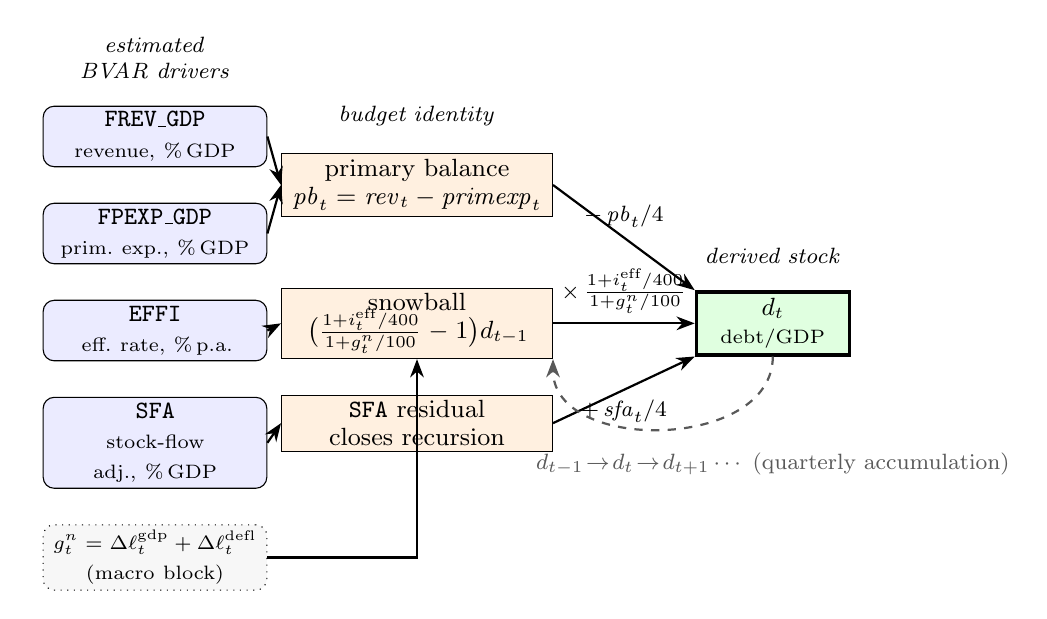
\begin{tikzpicture}[
    >=Stealth, node distance=4.5mm,
    font=\small,
    driver/.style={draw, rounded corners, fill=blue!8, minimum height=6.5mm,
                   text width=27mm, align=center, inner sep=2pt},
    iden/.style={draw, fill=orange!12, minimum height=6.5mm,
                 text width=33mm, align=center, inner sep=2pt},
    stock/.style={draw, very thick, fill=green!12, minimum height=8mm,
                  text width=18mm, align=center, inner sep=2pt},
    op/.style={font=\footnotesize},
    flow/.style={->, thick},
    lag/.style={->, dashed, thick, gray!70!black}
  ]

  % --- Estimated BVAR drivers (left column) ---
  \node[driver] (rev)  {\texttt{FREV\_GDP}\\\scriptsize revenue, \%\,GDP};
  \node[driver, below=of rev]  (exp) {\texttt{FPEXP\_GDP}\\\scriptsize prim.\ exp., \%\,GDP};
  \node[driver, below=of exp]  (eff) {\texttt{EFFI}\\\scriptsize eff.\ rate, \%\,p.a.};
  \node[driver, below=of eff]  (sfa) {\texttt{SFA}\\\scriptsize stock-flow adj., \%\,GDP};

  \node[above=2.2mm of rev, font=\footnotesize\itshape, text width=30mm, align=center]
       {estimated BVAR drivers};

  % --- Budget-identity terms (middle column) ---
  \coordinate (revexp) at ($(rev)!0.5!(exp)$);
  \node[iden, right=16mm of revexp] (pb)
       {primary balance\\[-1pt]$\mathit{pb}_t=\mathit{rev}_t-\mathit{primexp}_t$};
  \node[iden, below=9mm of pb] (snow)
       {snowball\\[-1pt]$\bigl(\tfrac{1+i^{\text{eff}}_t/400}{1+g^{n}_t/100}-1\bigr)d_{t-1}$};
  \node[iden, below=of snow] (res)
       {\texttt{SFA} residual\\[-1pt]closes recursion};

  \node[above=2.2mm of pb, font=\footnotesize\itshape, text width=34mm, align=center]
       {budget identity};

  % nominal growth feed (from macro block)
  \node[draw, dotted, rounded corners, fill=gray!6, text width=27mm, align=center,
        inner sep=2pt, below=of sfa]
       (gn) {\scriptsize $g^{n}_t=\Delta\ell^{\text{gdp}}_t+\Delta\ell^{\text{defl}}_t$\\(macro block)};

  % --- Debt stock recursion (right column) ---
  \node[stock, right=18mm of snow] (dt)
       {$d_t$\\[-1pt]\scriptsize debt/GDP};

  \node[above=2.2mm of dt, font=\footnotesize\itshape, text width=22mm, align=center]
       {derived stock};

  % driver -> identity flows
  \draw[flow] (rev.east) -- (pb.west);
  \draw[flow] (exp.east) -- (pb.west);
  \draw[flow] (eff.east) -- (snow.west);
  \draw[flow] (sfa.east) -- (res.west);
  \draw[flow] (gn.east) -| (snow.south);

  % identity -> stock recursion (terms of eq.~debt)
  \draw[flow] (pb.east)   -- node[op, above]{$-\,\mathit{pb}_t/4$} (dt.north west);
  \draw[flow] (snow.east) -- node[op, above]{$\times\,\tfrac{1+i^{\text{eff}}_t/400}{1+g^{n}_t/100}$} (dt.west);
  \draw[flow] (res.east)  -- node[op, below]{$+\,\mathit{sfa}_t/4$} (dt.south west);

  % --- accumulation across quarters: lagged debt feedback ---
  \draw[lag] (dt.south) .. controls +(0,-12mm) and +(0,-12mm) .. (snow.south east);
  \node[font=\footnotesize, gray!70!black, align=center, below=11mm of dt.south, anchor=north]
       {$d_{t-1}\!\rightarrow\! d_t\!\rightarrow\! d_{t+1}\cdots$ (quarterly accumulation)};

\end{tikzpicture}
\caption{Fiscal stock-flow schematic. The four estimated BVAR drivers
(\texttt{FREV\_GDP}, \texttt{FPEXP\_GDP}, \texttt{EFFI}, \texttt{SFA};
Section~\ref{sec:drivers}) feed the budget identity: revenue and
primary expenditure form the primary balance $\mathit{pb}_t$
(\S\ref{sec:drivers}); the effective rate \texttt{EFFI} and nominal growth
$g^{n}_t$ \eqref{eq:gn} form the interest--growth \emph{snowball}
\eqref{eq:snowball}; and the estimated \texttt{SFA} enters as the
residual that closes the recursion. These flows accumulate into the derived
debt-to-GDP stock $d_t$ by the quarterized roll-forward
$d_t = d_{t-1}\,(1{+}i^{\text{eff}}_t/400)/(1{+}g^{n}_t/100)
- \mathit{pb}_t/4 + \mathit{sfa}_t/4$ \eqref{eq:debt}, with the lagged
stock $d_{t-1}$ fed back each quarter (dashed). Debt is \emph{derived}, never
estimated (\texttt{computeFiscalBlock}, Section~\ref{sec:debtrec}).}
\label{fig:fiscal}
\end{figure}

Let $d_t$ denote debt-to-GDP in percent, $i^{\text{eff}}_t$ the
effective rate in percent per annum, and $g^{n}_t$ the \emph{quarterly}
nominal growth rate in decimal, read off the level-space forecast as
\begin{equation}\label{eq:gn}
  g^{n}_t \;=\;
  \tfrac{1}{100}\Bigl[
   \bigl(\ell^{\text{gdp}}_t - \ell^{\text{gdp}}_{t-1}\bigr)
 + \bigl(\ell^{\text{defl}}_t - \ell^{\text{defl}}_{t-1}\bigr)\Bigr],
\end{equation}
the sum of the real-GDP and deflator log differences in the stored
$100\ln$ space, divided by $100$ (a bloc whose GDP series were nominal
would omit the deflator term via the \texttt{gdpIsNominal} switch; no
shipped bloc currently uses it). With the primary balance
$\mathit{pb}_t = \mathit{rev}_t - \mathit{pexp}_t$ (percent of GDP,
annual, positive $=$ surplus), the debt stock rolls forward one quarter
as
\begin{equation}\label{eq:debt}
  d_t \;=\; d_{t-1}\,
     \frac{1 + i^{\text{eff}}_t/400}{1 + g^{n}_t}
     \;-\; \frac{\mathit{pb}_t}{4}
     \;+\; \frac{\overline{\mathit{sfa}}}{4},
  \qquad d_{-1} \equiv d_0,
\end{equation}
exactly as coded: the annual rate quarterized by $400$, the quarterly
decimal growth entering directly, and one quarter's worth of the annual
flow ratios accruing per step. The quarterly convention is pinned by a
back-cast test that reconstructs the observed debt ratio from realized
drivers. Two derived flows complete the identity: the interest bill
$\mathit{int}_t = i^{\text{eff}}_t\, d_{t-1}/100$ (annual, percent of
GDP) and the deficit $\mathit{def}_t = \mathit{int}_t - \mathit{pb}_t$.
Subtracting $d_{t-1}$ from~\eqref{eq:debt} isolates the automatic
\emph{snowball} from the discretionary balance,
\begin{equation}\label{eq:snowball}
  \Delta d_t
  = \underbrace{\Bigl(\frac{1 + i^{\text{eff}}_t/400}{1 + g^{n}_t} - 1\Bigr) d_{t-1}}_{\text{snowball (interest--growth)}}
  \;-\; \frac{\mathit{pb}_t}{4} \;+\; \frac{\overline{\mathit{sfa}}}{4}
  \;\approx\;
  \frac{i^{\text{eff}}_t/400 - g^{n}_t}{1 + g^{n}_t}\, d_{t-1}
  \;-\; \frac{\mathit{pb}_t}{4} \;+\; \frac{\overline{\mathit{sfa}}}{4},
\end{equation}
the quarterized $(i-g)$ form: debt rises mechanically whenever the
quarterized effective rate exceeds quarterly nominal growth.

\begin{remark}[The SFA in the roll-forward is the structural constant]\label{rem:sfa}
Equation~\eqref{eq:debt} deliberately uses the constant
$\overline{\mathit{sfa}} = \texttt{sfaDefault}$, \emph{not} the
forecast \texttt{SFA} column, even though the column is estimated and
displayed with its own chart, dynamics, and bands. The forecast column
responds to everything else in the VAR --- including long-run anchors'
cross-responses --- and can be dragged to spurious extremes that would
distort the derived debt path; the long-run mean is the economically
correct closure for a projection. The \texttt{SFA} \emph{chart} shows
the model's forecast of the discrepancy; the debt \emph{arithmetic}
uses the stable constant. Conditioning the SFA chart is still
meaningful --- it moves the rest of the system through the estimated
covariances --- but it does not enter~\eqref{eq:debt}.
\end{remark}

The recursion~\eqref{eq:gn}--\eqref{eq:snowball} is
\texttt{computeFiscalBlock}, the only fiscal recursion wired to the
charts: it produces the baseline, scenario, and counterfactual debt
paths and, run per posterior draw, the fiscal bands. It is
\emph{passive}: lagged debt enters every term, so a single forward sweep
is exact, and there is no debt feedback onto the primary balance or the
rate --- the displayed balance is exactly
$\mathit{rev}_t - \mathit{pexp}_t$ and the displayed rate exactly the
BVAR forecast. Three derived charts are displayed, in a row labelled
\ui{Fiscal block --- derived by accounting identity}: the
\ui{Primary Balance}, the per-quarter change \ui{$\Delta$ Debt-to-GDP}
(a pure identity output, not conditionable), and \ui{Debt-to-GDP}.
The remaining identity outputs (interest, deficit, overall balance,
snowball) are computed internally but not charted.

\begin{remark}[Timing of the debt ratio]\label{rem:debttiming}
The denominator convention follows GFSM\,2014 and the Eurostat quarterly Maastricht series:
$d_t$ is the \emph{end-of-quarter} gross debt stock divided by \emph{contemporaneous rolling-annual}
nominal GDP, $d_t = D_t/\sum_{s=t-3}^{t} Y_s$ --- the four-quarter sum \emph{ending in} quarter $t$,
not lagged GDP. All fiscal ratios (\texttt{FREV\_GDP}, \texttt{FPEXP\_GDP}, debt/GDP) use the same
contemporaneous four-quarter denominator, and $d_0$ is seeded at the last observed debt stock over
the four quarters ending at that observation. The one deliberately \emph{lagged} object is the
effective rate, $\texttt{EFFI}_t = 400\,\mathit{int}_t/D_{t-1}$: interest accrues on the
pre-existing stock, the financial-programming convention. In the roll-forward \eqref{eq:debt} the
denominator's growth enters through the factor $(1+i^{\text{eff}}_t/400)/(1+g^{n}_t/100)$ with
$g^{n}_t$ the quarterly nominal-GDP growth of the same quarter; in sample, any wedge between
quarterly growth and the rolling-sum growth is absorbed into the estimated \texttt{SFA} residual
by construction, so the identity holds to machine precision on history.
\end{remark}

\begin{remark}[Coupon-lumpy blocs: even interest distribution]\label{rem:evencoupon}
For eight blocs whose recorded interest payments follow an annual or
semiannual coupon calendar --- \texttt{EVEN\_INTEREST} $=$ \{CL, CO, CR,
ID, IL, MX, TR, ZA\}, identified by a systematic within-year pattern in
the raw interest flows (calendar-$R^2 > 0.5$ with coefficient of
variation $> 0.25$, or near-perfect quarterly alternation) --- the lumpy
coupon would otherwise inject a mechanical sawtooth into
$\texttt{EFFI}_t = 400\,\mathit{int}_t/D_{t-1}$. Before estimation the
four quarterly interest payments \emph{within each complete calendar
year} are replaced by their common mean, so the annual interest total is
preserved \emph{exactly} (a trailing partial year uses the
trailing-four-quarter mean); \texttt{EFFI} then measures the
\emph{accrual} borrowing cost rather than the cash-settlement spike.
Primary expenditure keeps the \emph{raw} interest --- total minus
interest, $\mathit{te}-\mathit{int}$, stays true non-interest spending
--- and the exact debt-identity residual \texttt{SFA} absorbs the
genuine cash-versus-accrual timing, which is why these blocs also carry
the seasonal dummies of Section~\ref{sec:seasonal}. The debt
roll-forward~\eqref{eq:debt} still closes to machine precision
($<10^{-14}$) (\texttt{pipeline/build\_fiscal22\_columns.py},
\texttt{even\_distribute\_years}). Empirically the evening removes the
\texttt{EFFI} sawtooth (mean absolute quarterly change falls from
$\sim\!5$ to $\lesssim 0.25$ points for CL, MX, ZA) and moves the
near-Nyquist companion root that drove it off $-1$ (e.g.\ ZA from
$-0.97$ to $-0.63$).
\end{remark}

\subsection{Targeting a debt or balance path}\label{sec:debttarget}

\begin{figure}[!ht]
\centering
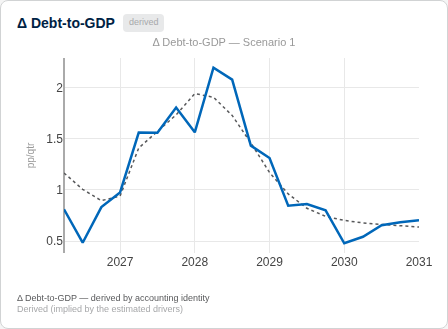
\includegraphics[width=0.55\textwidth]{manual_figs/ui_debt_panel.png}
\caption{The derived debt block under the tightening scenario: the quarterly change in debt-to-GDP
(solid) rises above baseline (dotted) as the snowball term absorbs the higher effective rate,
then reverts. Debt panels are conditionable: right-click pins a point, dragging sets a target
path, and the smoother back-solves the primary balance that delivers it
(\S\ref{sec:debttarget}).}
\label{fig:ui-debt}
\end{figure}


The recursion also runs backward. Given a target debt path
$\{d^{\text{tgt}}_t\}$, the primary balance required at each quarter is
the exact inverse of~\eqref{eq:debt},
\begin{equation}\label{eq:reqpb}
  \mathit{pb}_t \;=\;
  4\left[\frac{d^{\text{tgt}}_{t-1} + \mathit{int}_t/4}{1 + g^{n}_t}
        \;-\; d^{\text{tgt}}_t\right]
  \;+\; \overline{\mathit{sfa}},
\end{equation}
with the lag taken along the target path and
$\mathit{int}_t = i^{\text{eff}}_t\, d^{\text{tgt}}_{t-1}/100$
(\texttt{requiredPrimaryBalance}). The tool evaluates the effective rate
and growth on the unconditional forecast, computes~\eqref{eq:reqpb},
and pins the combination
$\mathit{rev}_t - \mathit{pexp}_t = \mathit{pb}_t$ as a
linear-combination constraint (Section~\ref{sec:kf}); the smoother finds
the most plausible revenue/expenditure mix.

\begin{example}[Drawing a debt path]\label{ex:debt}
On a fiscal economy, right-click the \ui{Debt-to-GDP} chart where the
path should pass --- on this chart the dragged value is the absolute
target, $100$ meaning $100$ percent of GDP --- and shape the trajectory;
right-click a quarter to pin or release it. A \ui{Primary Balance}
target set the same way is hit \emph{exactly} (it is one linear
constraint). A \ui{Debt-to-GDP} target is hit \emph{approximately}: the
inversion~\eqref{eq:reqpb} conditions on the model's unconditional rate
and growth, which themselves respond a little to the implied
consolidation, and the tool does not iterate on that feedback --- expect
a miss of up to a point or so of GDP over the horizon. For an exact
decimal the instrument is the balance target; for a coherent
consolidation scenario the debt target is the natural handle. Note that
conditioning \emph{any} fiscal variable implicitly conditions the
derived row --- a note next to the block header says so.
\end{example}

\begin{remark}[Fiscal bands are identity-consistent, and re-centred]\label{rem:fiscalbands}
Each band draw pushes its own simulated drivers
through~\eqref{eq:debt}, so the debt band widens exactly as fast as the
underlying budget-and-growth uncertainty implies. Because the
roll-forward compounds, the per-draw debt distribution is right-skewed:
its median sits below the debt path computed at the mean drivers, which
would leave the central line hugging the band's upper edge. At render
the band is therefore re-centred --- each quarter's band midpoint is
shifted onto the displayed path, preserving the band's width and
asymmetry (the fan-chart convention ``central projection $\pm$
uncertainty''); at actively pinned quarters the band collapses onto the
line. The same treatment applies to the external position below.
\end{remark}

%% ================================================================
\section{The external accounts}\label{sec:external}
%% ================================================================

Three economies --- the United States, the euro area, and China ---
carry an external block that derives the trade balance, the current
account, and the net foreign asset (NFA) position from the estimated
trade, price, and exchange-rate variables by the balance-of-payments
identity (\texttt{app/src/lib/compute/externalAccounting.ts}). All
three charts are read-only (\ui{derived} badges): to move them,
condition the drivers --- exports, imports, the exchange rate, growth
--- and the external row follows.

With $b_t$ the NFA-to-GDP ratio in percent, seeded at the latest
published net international investment position ($b_{-1} \equiv
\mathit{nfa}_0$: US $-66.75$, EA $+11.0$, CN $+20.35$ percent of GDP at
the current vintage), the per-quarter identity as coded is
\begin{align}
  \mathit{tb}_t &= 100\,\frac{X_t - M_t}{Y_t},
  &\mathit{ca}_t &= \mathit{tb}_t + \frac{i^{\textsc{nfa}}\, b_{t-1}}{100},
  \label{eq:tbca}\\[2pt]
  \mathit{val}_t &= -\,\phi^{\textsc{fx}}\, b_{t-1}\,
      \frac{\Delta \ell^{\textsc{fx}}_t}{100},
  &b_t &= \frac{b_{t-1}}{1 + g^{n}_t}
      \;+\; \frac{\mathit{ca}_t}{4} \;+\; \mathit{val}_t,
  \label{eq:nfa}
\end{align}
where $X_t, M_t, Y_t$ are the exponentiated export, import, and GDP
levels (for the US and the euro area a real-trade-to-real-GDP ratio,
validated against the published balance-of-payments ratios; for China a
deflated real index with the shipped scale factors, monthly trade
aggregated to quarterly), $\Delta\ell^{\textsc{fx}}_t$ is the quarterly
change of the $100\ln$ effective exchange rate (positive $=$ home
appreciation, which shrinks the home-currency value of net foreign
assets --- hence the sign), and $g^n_t$ is quarterly nominal growth
as in~\eqref{eq:gn}. The stock update divides the inherited ratio by
$(1+g^n_t)$ --- the automatic denominator effect --- adds one quarter of
the annual current account, and adds the valuation term; the return on
the stock enters through the income term of $\mathit{ca}_t$, computed on
the undiluted lagged ratio (the second-order cross-terms this drops are
noted in the code header).

Two inputs are stated modelling assumptions, not estimates, and are
flagged as such in the shipped metadata: the return on net foreign
assets $i^{\textsc{nfa}} = 3$ percent per annum, and the share of the
position exposed to the exchange rate $\phi^{\textsc{fx}} = 0.4$. Treat
the \emph{level} of the income and valuation terms as indicative and
their direction as the reliable part.

%% ================================================================
\section{Long-run anchors}\label{sec:longrun}
%% ================================================================

The long-horizon behaviour of the forecasts is inherited from the
estimated VAR, whose level dynamics carry roots on or near the unit
circle; the far end of a projection can therefore drift away from any
value the user regards as a credible steady state --- a two-percent
inflation objective, a potential growth rate, a stable revenue ratio.
The \ui{Long-run targets} panel lets the user pin the terminal forecast
of a chosen variable to a number, exactly and instantly. The mechanism
is a deterministic counterfactual on the companion drift in the spirit
of \citet{Villani2009}, implemented in
\texttt{app/src/lib/compute/driftSetter.ts}.

\paragraph{The shipped consensus set.} The tool ships a reviewed default anchor set
(\texttt{default\_anchors.json}; July-2026 transition-default revision: 35 anchors across 28 blocs)
tuned under the now-default steady-state transition. Because that path phases the adjustment in
rather than shifting the whole path, the set is anchored to \emph{official} long-run values wherever
the model shows a genuine terminal gap --- central-bank inflation targets throughout (euro-area
members at the ECB's two per cent, national targets elsewhere), medium-term potential growth where
the raw path is clearly off, and the effective-rate / revenue / expenditure trio on fiscal blocs.
This is a real gain of the transition shape: sixteen of these official-target anchors (Czechia,
Norway, Portugal, Thailand, Russia, Sweden and more, all to two-to-four per cent) are rejected as
harmful under the rigid shift, which would jump their near term, and all are clean under the
transition. Anchors are admitted only if the sensitivity clears the guard of \S\ref{sec:drift}, and
the shipped set is verified by the smell test (\texttt{anchor\_smell.mjs}) and locked by a
panel-wide non-explosiveness regression. Two guards still bite --- both shape-independent, being
properties of the estimated steady state rather than the path: a target that lands within the
redundancy threshold of the model's own terminal is dropped, and one that would displace an
unanchored headline variable by more than a point at the terminal is dropped or co-anchored. The
euro-area primary-expenditure anchor stays removed for the second reason (its cross-drag drives the
euro-area policy-rate terminal negative). A handful of high-inflation emerging markets --- Colombia,
Hungary, T\"urkiye, Israel, Malaysia --- are shipped model-driven and flagged: their estimates link
inflation and growth so tightly that pinning one drags the other several points at the steady state,
which no univariate anchor and no choice of path can repair; these await re-sourcing or a joint
re-estimation. Argentina (hyperinflation decay) and Japan (anchors disabled) also ship unanchored.

\subsection{The drift setter}\label{sec:drift}

Write the deterministic part of the companion
recursion~\eqref{eq:ss} as $Y_{T+h} = T^{h} Y_T + S_h\, c_\alpha$ with
\begin{equation}\label{eq:Sh}
  S_h = \sum_{k=0}^{h-1} T^{k},
\end{equation}
the partial sum of companion powers, built once per bloc ($H$
matrix products, cached). A shift $\delta c$ of the drift moves the
forecast by exactly $\Delta Y_{T+h} = S_h\,\delta c$ --- an algebraic
identity, verified against the iterated recursion to $10^{-11}$. We
deliberately avoid the closed-form steady state
$(I - \sum_\ell B_\ell)^{-1} c$: for near-unit-root level VARs that
matrix is near-singular and the ``steady state'' a meaningless number of
order $10^{5}$, whereas the finite-horizon operator~\eqref{eq:Sh} is
well posed. A target on variable $j$ shifts only $j$'s own equation,
$\delta c = e_j\,\delta c_j$, and the coherent system-wide response is
the $j$-th column, $\Delta Y_{T+h} = S_h[:,j]\,\delta c_j$. The scalar
is chosen so the \emph{displayed} terminal forecast lands on the target
$\psi^\star_j$:
\begin{equation}\label{eq:sens}
  \delta c_j = \frac{\psi^\star_j - \psi^{0}_j}{\mathrm{sens}_j},
  \qquad
  \mathrm{sens}_j =
  \begin{cases}
    4\bigl(S_H[j,j] - S_{H-1}[j,j]\bigr), & \texttt{log} \text{ variable},\\[2pt]
    S_H[j,j], & \texttt{lin} \text{ variable},
  \end{cases}
\end{equation}
with $\psi^{0}_j$ the current terminal display forecast --- the
slider's default position, so an unmoved slider is a byte-exact no-op. A
variable whose own sensitivity is below the guard
$|\mathrm{sens}_j| < 0.3$ has its slider disabled (``near-singular
response''): forcing a target there would require an explosive drift.

\paragraph{Two paths to the target: steady-state transition (default) or
rigid shift.} Equation~\eqref{eq:sens} fixes \emph{how far} the terminal
must move; a second choice --- the \ui{Path to target} toggle --- fixes
\emph{how the adjustment is distributed across the horizon}. The
constant-drift response $\Delta Y_{T+h}=S_h[:,j]\,\delta c_j$ places the
\emph{entire} effect from the first forecast quarter: because $S_1=I$, a
growth variable's displayed deviation at $h=1$ is $4\,\delta c_j$ --- the
\emph{full} terminal gap, applied at once and held flat. This
\ui{rigid shift} is exact at the terminal and band-coherent, but it
\emph{jumps} the near term at the origin and, for a large gap, can
manufacture a near-term contraction or deflation. The shipped default is
instead a \ui{steady-state transition}: the same terminal $\delta c_j$ is
phased in along the anchored variable's own estimated convergence profile
\begin{equation}\label{eq:transition}
  w_j(h) = \frac{S_h[j,j]}{S_H[j,j]},
  \qquad w_j(1)\approx \tfrac{1}{S_H[j,j]}\approx 0,\quad w_j(H)=1,
\end{equation}
so the near term stays data-consistent (no origin jump) and the forecast
\emph{glides} to the target by the end of the horizon at the model's own
mean-reversion speed. This is the reactive, no-re-estimation counterpart
of a steady-state (mean-adjusted) prior in the spirit of
\citet{Villani2009}: rather than translating the mean path by a constant,
it lets the estimated dynamics carry the forecast from the observed edge
to the long-run target. It is finite-horizon by construction --- the
identity $I-T^h = (I-T)\,S_h$ shows $w_j$ is exactly the normalised
$(I-T^h)$ operator --- so it never touches the singular level steady
state $(I-\sum_\ell B_\ell)^{-1}c$ that motivated~\eqref{eq:Sh}. The
terminal is identical to the rigid shift, so anchored targets are hit
under either path; only the near-to-medium term differs. Each horizon is
still a rigid translation, so band widths remain invariant
(Remark~\ref{rem:bandrigid}). Cross-variable drag phases in at the source
anchor's rate applied to the exact terminal cross-response.

\paragraph{Several targets: per-variable or joint.} With two or more
targets the cross-responses interfere --- a drift on equation $j$ moves
every other anchored terminal through $S_H[k,j]$. The panel exposes a
\ui{Multiple-target solve} toggle:
\begin{itemize}
  \item \ui{Per-variable} (the default): each
    $\delta c_k$ from its own diagonal sensitivity~\eqref{eq:sens}.
    Stable and bounded, but approximate --- it ignores the
    cross-responses, so with several targets each terminal lands
    slightly off its stated value.
  \item \ui{Joint}: solve the $K \times K$ display-unit system
    $M^{\text{lr}}\,\delta c = \psi^\star - \psi^{0}$, whose diagonal is
    exactly~\eqref{eq:sens}, by Gaussian elimination with partial
    pivoting. Every anchored terminal then lands exactly --- but a
    near-collinear target set (say two anchored interest rates the
    dynamics cannot separate in the long run) makes the system
    ill-conditioned: the exact solution buys terminal precision with
    huge offsetting drifts (measured up to $|\delta c| \approx 459$
    where the diagonal needed $\approx 11$) that wreck the path
    elsewhere. A singular system falls back to per-variable
    numerically; an ill-conditioned but solvable one is returned and
    \emph{flagged} (the joint drift exceeding twice the per-variable
    maximum trips the flag), and the user is expected to switch back.
\end{itemize}
Per-variable is the shipped default. The near-term-implausibility that
once accompanied a large gap --- at the 2026Q1 origin, anchoring the US
deflator (model terminal $4.3$ against the $2.0$ target) once displayed a
$-2.1$ point disinflation shock at the first forecast quarter --- was the
signature of the \emph{rigid shift}; the steady-state transition of
\eqref{eq:transition} removes it, gliding the same series from $3.5$
smoothly down to $2.0$ with a first-quarter move of under a tenth of a
point. The two toggles are orthogonal: the solve mode (per-variable /
joint) sets \emph{how far} each terminal moves; the path (transition /
rigid) sets \emph{how the move is phased in}.

\paragraph{Bands, fiscal forwarding, and visibility.} The response
$\Delta Y$ is added identically to the central path and to every shipped
band quantile --- a rigid translation, widths provably invariant
(Remark~\ref{rem:bandrigid}) --- and, in level space, forwarded into the
fiscal recursion~\eqref{eq:debt}, so the debt path responds coherently:
a real-growth target owns the direction of the debt ratio through the
$(i-g)$ snowball, which is why its row carries the tag \ui{sets debt
path}. Judgment is flagged: the affected chart title turns amber with a
\ui{judgement} badge stating target and estimate, and the grid-level
status line counts the anchored variables. Every control starts at the
model estimate, and clearing all targets restores the raw model
byte-exactly.

\paragraph{Consensus preset.} Blocs with publicly defensible long-run
values carry an \ui{Apply consensus anchors} preset --- deliberately
minimal (35 anchors across 28 economies at the July-2026 transition
revision): potential growth and the inflation objective per economy, plus
the effective-rate/revenue/expenditure trio for fiscal blocs; never
policy rates, unemployment, or asset prices, whose collinear anchors would
ill-condition the joint system. Each kept anchor was individually
verified --- under the shipped transition path --- to fix a genuine
terminal bias without displacing another headline variable. Where a preset
ships it is on by default and fully reversible (\ui{Clear}); the
model-driven-and-flagged economies of the preceding paragraph ship none
and stay entirely model-driven.

\paragraph{On a coupled bloc the target is marginal.} The drift setter
operates on one bloc's companion. On a GVAR economy it shifts that
bloc's own long run; partners are not re-solved unless the second
spillover switch, \ui{Long-run target spillovers (GVAR constant
shifts)}, is on. That channel is instant --- the drift deviation enters
the coupled system only through the forcing term $d$
of~\eqref{eq:fp}, leaving $M$ and its precomputed inverse untouched, and
the receiving country's banner turns amber with
\ui{+ spillover from \dots} naming the origin --- judgment stays visible
across borders.\label{sec:driftgvar}

\subsection{The in-prior long-run prior}\label{sec:plr}

A second, offline mechanism exists: the ``prior for the long run''
(PLR) of \citet{GiannoneLenzaPrimiceri2019}, which augments the prior of
Section~\ref{sec:prior} with dummy observations shrinking a set of
long-run linear combinations $Hy$ toward non-cointegration. It is a
proper Bayesian prior --- it changes the posterior and requires
re-estimation --- and is therefore part of the estimation pipeline, not
the browser. A US head-to-head (run on an earlier, pre-expansion
$n=36$ US specification; the deployed bloc is $n=40$) found the PLR
acts mainly on the \emph{bands}, tightening the GDP-growth 68\% band by
about $7$ percent at unit tightness, while leaving the central long-run
path essentially unchanged --- the appropriate instrument for principled
band tightening, not for pinning a terminal to a chosen number. The two
mechanisms are complementary: to pin a long run interactively, use the
drift setter; for disciplined bands, the PLR.

\begin{remark}[A retired mechanism]\label{rem:tilt}
An earlier release pinned long runs by entropic tilting
\citep{RobertsonTallmanWhiteman2005} --- reweighting the posterior draws
so the weighted terminal moment hits the target. It degenerated in
practice: as the target moved away from the draw cloud the effective
sample size $1/\sum_d w_d^2$ collapsed toward one (a joint 13-constraint
tilt reached $\mathrm{ESS} \to 1$ at $D=500$), leaving the anchored band
resting on a handful of draws precisely where the user most wanted a
firm answer. The drift setter replaced it wholesale --- deterministic,
exact at any target, instant --- and the tilt is no longer wired to any
interface control (its module remains in the repository, exercised only
by its unit test).
\end{remark}

%% ================================================================
\section{Policy counterfactuals}\label{sec:counterfactual}
%% ================================================================

A scenario asks what happens if the data come in differently; a policy
counterfactual asks what a \emph{deliberate policy change} would cause.
The distinction is identification: the smoother's response to a pinned
rate path is the estimated historical co-movement, which cannot tell a
policy surprise from a response to something else. The counterfactual
layer therefore borrows structure from a DSGE model of the user's
choice, drawn from the Macroeconomic Model Data Base
\citep[MMB;][]{WielandCwikMuellerSchmidtWolters2012,
WielandAfanasyevaYooKuete2016}, and overlays its identified responses on
the scenario.

\subsection{Impulse responses and shock inversion}\label{sec:inversion}

The MMB catalogue in the tool lists 169 models; pre-computed impulse
responses ship for 155 of them, each under up to nine interest-rate
rules (Taylor, Smets--Wouters, CEE, Gerdesmeier--Roffia,
Levin--Wieland--Williams, two Orphanides--Wieland variants, Coenen,
Christiano--Motto--Rostagno). A model--rule pair is one JSON file of
responses to a monetary (and, where the model has a fiscal sector, a
government-spending) shock, with the rule embedded in the model's
equilibrium when the responses were generated --- the tool never
evaluates a policy rule at run time. Rules without computed responses
for the selected model are greyed out.

Let $h_r(s)$ denote the interest-rate response at horizon $s$ to a unit
monetary shock. Given a user rate adjustment $\Delta r_t$ on a set of
\emph{constrained} quarters, the tool solves for the shock sequence by
forward substitution on the lower-triangular Toeplitz system --- a new
shock only where the user pinned, zero elsewhere:
\begin{equation}\label{eq:inversion}
  \varepsilon_t =
  \begin{cases}
    \dfrac{\Delta r_t - \sum_{j<t} h_r(t-j)\,\varepsilon_j}{h_r(0)},
      & t \text{ constrained},\\[6pt]
    0, & \text{otherwise},
  \end{cases}
\end{equation}
so at unconstrained quarters the rate follows the decaying response of
the earlier shocks --- the model's rule, not a snap-back. The implied
inflation and output responses are the convolutions
$\Delta\pi_t = \sum_{j\le t} h_\pi(t-j)\,\varepsilon_j$ and
$\Delta y_t = \sum_{j\le t} h_y(t-j)\,\varepsilon_j$; a parallel
inversion runs on the fiscal shock for the spending sliders.

\subsection{Re-conditioning and the response modes}\label{sec:cfmodes}

\begin{figure}[!ht]
\centering
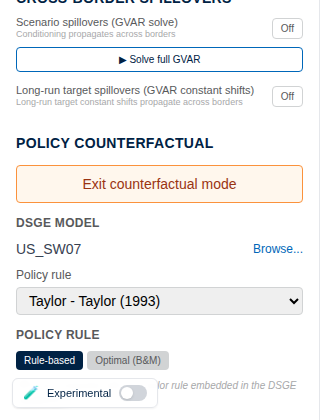
\includegraphics[width=0.42\textwidth]{manual_figs/ui_cf_controls.png}
\caption{The counterfactual control rail: entering counterfactual mode selects the DSGE model
(here \textsc{us\_sw07}) and the policy rule --- a named rule (Taylor 1993) or the
optimal rule of \S\ref{sec:bm} --- whose impulse responses are layered on the BVAR scenario as
described in \S\ref{sec:inversion}.}
\label{fig:ui-cf}
\end{figure}


The counterfactual is not an additive overlay of every variable: the
DSGE deltas are imposed on the \emph{key} variables and the BVAR fills
in the rest. The \ui{Macro response} selector offers two modes:
\begin{itemize}
  \item \ui{DSGE/Taylor-rule (IRF-consistent)} (default): the rate is
    pinned at scenario plus $\Delta r$, inflation and output at scenario
    plus the DSGE deltas; all other variables are re-conditioned through
    the smoother, so the responses are consistent with both the
    identified transmission and the estimated covariances. One
    convention subtlety is handled per variable: the MMB inflation
    response is a \emph{rate} (cumulated into the $100\ln$ price level,
    $\sum_{s\le t}\Delta\pi_s/4$), the output-gap response a percent
    \emph{level} deviation (applied directly, not cumulated), and a rate
    response an identity.
  \item \ui{BVAR-endogenous (let adjust)}: only the rate path is pinned;
    everything else responds through the estimated co-movements, exactly
    as in a scenario. The two modes answer different questions ---
    ``what does this theory say the move would do'' versus ``what
    usually accompanies such a path'' --- and their disagreement is
    informative. If the selected pair has no computed responses the tool
    falls back to this mode and says so in an amber notice.
\end{itemize}
In both modes the displayed counterfactual is the scenario plus the
smoother delta between the counterfactual pass and a reference pass with
zero adjustment, converted to display units by the conventions of
Section~\ref{sec:delta}; a zero adjustment reproduces the scenario
exactly.

\subsection{Reading the result}\label{sec:cfread}

The counterfactual draws as a dashed line in a distinct rust colour on
every chart; the scenario line stays put. To isolate the policy effect,
set \ui{Units} to \ui{\% vs base}; in that view the \ui{Level} $\mid$
\ui{Rate (IRF)} toggle selects between the cumulative effect on the
\emph{level} of each variable (the ``\% chg.''\ reporting convention)
and the quarter-by-quarter response in native units --- the latter
reproduces the MMB's own IRF plots exactly, since differencing the
cumulated log-level deviation and scaling by four recovers the rate
response. Uncertainty bands, when computed, belong to the scenario; the
counterfactual is a single model-implied path.

\begin{remark}[The rule choice is a first-order magnitude decision]\label{rem:rulescale}
The same one-quarter rate move can have an order-of-magnitude different
effect across rules. In the shipped responses of the default US model
(\texttt{US\_SW07}, \citealp{SmetsWouters2007}), the peak inflation
response to a unit monetary shock under the model's own Smets--Wouters
rule is about $32$ times the response under the Taylor rule, the output
response about $6$ times. Treat pass-through magnitudes as
model-and-rule dependent, never as a fact; flipping the model while the
scenario stays put (each scenario tab carries its own model and rule) is
the cheapest robustness check in the tool.
\end{remark}

\subsection{Optimal policy}\label{sec:bm}

Instead of hand-crafting the path, \ui{Optimal (B\&M)} computes it from
the same sufficient statistics, following
\citet{BarnichonMesters2023}: choose the shock sequence
$\varepsilon$ minimizing the quadratic loss
\begin{equation}\label{eq:bmloss}
  \mathcal{L} = \sum_{t=1}^{H}\Bigl[
    \lambda_\pi\bigl(\pi_t - \pi^\star\bigr)^2
    + \lambda_y\bigl(y_t - y^\star\bigr)^2\Bigr]
\end{equation}
subject to the linear IRF mapping. Stacking the weighted Toeplitz
operators, the minimizer is the Tikhonov-regularized least squares
\begin{equation}\label{eq:bmsolve}
  \varepsilon^\star
  = \bigl(\tilde{\mathcal H}'\tilde{\mathcal H} + \alpha I\bigr)^{-1}
    \tilde{\mathcal H}'\,\tilde b,
  \qquad
  \tilde{\mathcal H} =
  \begin{pmatrix}\sqrt{\lambda_\pi}\,\mathcal H_\pi\\
                 \sqrt{\lambda_y}\,\mathcal H_y\end{pmatrix},
  \quad \alpha = 10^{-6},
\end{equation}
with the implied rate path $\Delta r^\star = \mathcal H_r\,
\varepsilon^\star$ handed to the IRF-consistent mode. One slider sets
the preference weights ($\lambda_\pi = 5w$,
$\lambda_y = 5(1-w)$); the $\pi^\star$ and $y^\star$ sliders set the
targets. Unlike a hand-set adjustment, the optimal path pins
\emph{every} quarter --- it is a full plan, not a one-off surprise.

A fiscal lever completes the block: twelve government-spending sliders
scale the model's fiscal responses on top of the scenario, for the
subset of models (fewer than half) that include a fiscal sector. For
projecting the public finances themselves, the fiscal block of
Section~\ref{sec:fiscal} is the instrument.

%% ================================================================
\section{Data, vintages, and updates}\label{sec:data}

\begin{table}[!ht]
\centering
\footnotesize
\caption{Repository layout. Estimation in \texttt{pipeline/} produces a
per-bloc JSON export; \texttt{port\_gvar\_exports.py} ports it into
\texttt{app/public/data/bvar/}; the front end and its compute kernels consume
that data and never re-estimate.}
\label{tab:repro:layout}
\begin{tabular}{@{}lp{8.6cm}@{}}
\toprule
\textbf{Top-level} & \textbf{Key contents} \\
\midrule
\texttt{pipeline/} (MATLAB + Python) &
  \texttt{export\_bvar\_gvar24\_loop.m} (GVAR--EM estimator);
  \texttt{build\_*.py} (FRED / Eurostat / BIS / ECB pulls, trade weights,
  fiscal drivers); \texttt{port\_gvar\_exports.py}; \texttt{\_verify/}
  ground-truth checks. \\
\addlinespace
\texttt{app/} (Next.js + compute) &
  \texttt{src/lib/compute/} (Durbin--Koopman, GVAR solve, fiscal accounting);
  \texttt{scripts/} (\texttt{precompute\_gvar\_coupling.mjs},
  \texttt{verify\_gvar24.mjs}, \texttt{invert\_coupling.\{m,py\}});
  \texttt{public/data/bvar/<CC>/} (the deployed JSON the app reads). \\
\addlinespace
\texttt{docs/} (manual + runbooks) &
  \texttt{MFFM\_User\_Manual.tex}; \texttt{REESTIMATING\_MODELS.md},
  \texttt{ADDING\_A\_COUNTRY.md}, \texttt{ARCHITECTURE\_FOR\_AI.md}. \\
\bottomrule
\end{tabular}
\end{table}
%% ================================================================

\subsection{Sources}\label{sec:sources}

No single provider supplies current quarterly data for the full roster,
so the panels are assembled bloc by bloc from a small number of source
families, wired by per-bloc build scripts
(\texttt{pipeline/build\_*.py}) and recorded, series by
series, in a machine-readable coverage manifest
(\texttt{coverage\_manifest.json} under \texttt{app/public/data/}) from
which the
roster table of Appendix~\ref{app:tables} is generated.
\begin{itemize}
  \item \textbf{FRED} supplies the entire US bloc with exact series
    identifiers, the China bloc (built from verified real FRED series,
    with quarterly real activity anchored on a chain-linked volume
    index), the four global commons, and the BIS credit and
    residential-property series redistributed through FRED.
  \item \textbf{Eurostat} supplies the EU and EFTA economies:
    chain-linked volumes (\texttt{namq\_10\_gdp}), HICP, unemployment,
    interest rates, effective exchange rates, house prices; euro members
    carry the ECB policy and lending rates.
  \item \textbf{OECD quarterly national accounts and national sources}
    supply the remaining OECD members and emerging markets, with policy
    rates from national central banks or the BIS.
  \item \textbf{IMF WEO} is a back-fill of last resort: where a bloc's
    genuine quarterly series end short of the common estimation window,
    annual WEO projections are temporally disaggregated to fill the
    macro tail (proportional-Denton within-year profiling, observed
    quarters held fixed). WEO never overrides observed data, and every
    bloc whose live tail is WEO-derived is flagged in the manifest and
    in \ui{Data \& coverage}.
  \item \textbf{Derived series} --- the stars, the effective interest
    rate, the stock-flow adjustment, the rest-of-euro-area aggregates
    --- are computed, not pulled (Sections~\ref{sec:stars}
    and~\ref{sec:fiscal}).
\end{itemize}
The \ui{Data \& coverage} dialog (top bar) lists, for the economy on
screen, every variable's source, coverage span, last observed quarter,
and caveats --- the on-screen rendering of the manifest. Amber entries
end before the panel origin and correspond exactly to the amber chart
tails.

\subsection{Vintage policy: estimate once, shift quarterly}\label{sec:vintage}

The shipped panels are the product of two clearly separated steps.
\emph{Estimation build}: every bloc harmonized to a common 2025Q4
endpoint, on which all coefficients, draws, weights, and the coupling
artifact were estimated and frozen. \emph{Observed refresh}: the live
panel then advances --- currently to a default last-historical quarter
of 2026Q1 --- by pulling each newly published quarter from the same
sources in the same transforms, with \emph{no} re-estimation: the
forecast re-anchors from the unchanged companion
(\texttt{app/scripts/refresh-quarter.mjs}, fail-closed per bloc).
Because the coupled system links economies row by row, the panel origin
is \emph{uniform}: at this writing every bloc's history ends at 2026Q1.
Blocs whose sources lag reach the origin through the amber, flagged
nowcast described next --- never through fabricated observations. The
one exception is Israel, whose statistics arrive with a long lag; its
charts run on Israel's own calendar, about a year behind the panel (a
documented row-offset approximation, flagged in
\ui{Data \& coverage}).

Within a data round the not-yet-published quarters of the remaining
series are \emph{nowcast} by the coupled system itself: the panel is
truncated to the last quarter at which every cell is observed, every
observed cell in the ragged window is pinned at its published value, and
one coupled solve (Section~\ref{sec:coupling}) delivers each missing
cell's conditional expectation given everything already observed
anywhere in the panel --- the star channel carries the leaders' releases
into the laggards' estimates. Observed cells are never altered; every
imputed cell carries a provenance flag and draws amber
(\texttt{nowcastCompletion.ts}). The label \ui{NC} in the conditioning
list is this nowcast quarter.

The \ui{Monitor} page (top bar) shows what each data round did: per
economy, the revision of the current-quarter estimate against what the
previous vintage predicted for it, split by channel ---
\ui{observed} (the economy's own release surprised) versus
\ui{cross-block} (the economy published nothing; the move is pure
transmission of partners' releases). Source restatements of history are
accepted as current best knowledge and logged in the same page.
Once a year, after the previous calendar year is fully published for
every economy, the whole system is re-estimated and the cycle restarts;
only then do the estimated relationships change.

%% ================================================================
\section{Evaluation}\label{sec:eval}
%% ================================================================

The system's forecasting performance is evaluated in a companion
repository (\texttt{em-bayesian-gvar-eval}) under a protocol designed
before the runs; this section summarizes the design and the realized
results. Two questions are asked: does the estimation apparatus ---
Bayesian shrinkage, COVID-as-missing, the EM star fixed point, the
endogenous US --- earn its keep out of sample, and what does the
endogenous US buy that a frozen anchor cannot deliver.

\subsection{Design}\label{sec:oosdesign}

\paragraph{Models.} Nine forecast densities are scored: the proposed
EM-Bayesian GVAR in its two variants (\texttt{emgvar\_endo}, the full
endogenous-US loop, and \texttt{emgvar\_frozen}, the frozen-anchor
ablation), six benchmarks estimated on the same truncated panels --- a
driftless random walk in the scored space, an AR($p$) per series
($p$ by AIC, iterated multi-step; \citealp{MarcellinoStockWatson2006}),
a single-country BVAR with the stars dropped (the value-of-coupling
ablation), the textbook fixed-weight OLS GVAR of
\citet{PesaranSchuermannWeiner2004} and
\citet{DeesDiMauroPesaranSmith2007} with no data augmentation (the
headline classical competitor), a single-pass Bayesian GVAR (the
value-of-EM ablation), and a Bayesian dynamic factor model --- plus a
sample-mean climatology sibling of the random walk.

\paragraph{Scheme.} Pseudo-real-time recursive expanding window on the
final vintage: quarterly origins 2010Q1--2024Q4 (60 raw origins; the
four 2020 origins are dropped from the headline tables, leaving 56),
horizons $h \in \{1,2,4,8\}$, three targets per bloc (real-GDP growth
and inflation in the $4\Delta$ scored space, the short rate in levels),
six headline blocs (US, EA, JP, UK, CA, CN). Look-ahead is excluded by
construction: every panel is truncated to the origin before any
transformation or star is built; trade weights are rolling, as-of-origin
three-year averages (the shipped 2021--2023 weights are forbidden in the
sweep); and the COVID mask is re-applied in-sample at every origin. The
proposed variants require a longer warm-up and score at up to 52
origins. Predictive densities use 200 retained draws per origin with a
stationarity backstop that discards explosive posterior draws.

\paragraph{Scoring.} Point accuracy by relative RMSE against the random
walk. Density accuracy by the continuous ranked probability score
(CRPS), the primary metric, computed from the draw ensemble by the
standard energy-form estimator
\begin{equation}\label{eq:crps}
  \widehat{\mathrm{CRPS}}
  = \frac{1}{m}\sum_{k=1}^{m}\lvert X_k - y\rvert
  - \frac{1}{2m^{2}}\sum_{k=1}^{m}\sum_{l=1}^{m}\lvert X_k - X_l\rvert
\end{equation}
\citep{GneitingRaftery2007}, which degrades gracefully at modest draw
counts; calibration by PIT histograms and interval coverage
\citep{Berkowitz2001}. Because most model pairs are \emph{nested},
predictive-ability inference uses the \citet{GiacominiWhite2006}
conditional test as the headline (valid under nesting and correct for
the expanding scheme), \citet{ClarkWest2007} for nested point
comparisons, and \citet{DieboldMariano1995} with the
\citet{HarveyLeybourneNewbold1997} correction only for non-nested pairs;
multiplicity is controlled by Romano--Wolf step-down
\citep{RomanoWolf2005}, and the per-cell \emph{model confidence set}
(MCS) of \citet{HansenLundeNason2011} reports which models are
statistically indistinguishable from the best.

\subsection{Results}\label{sec:oosresults}

On \emph{point} accuracy the univariate AR($p$) and the factor model
lead --- a familiar macro-forecasting result --- and the EM-GVAR does
not win the horse race outright. The decisive evidence is in the density
comparison and the MCS: the EM-Bayesian GVAR sits \emph{inside} the 90\%
MCS for \textbf{inflation at every horizon} and for the \textbf{short
rate at $h \le 4$} --- statistically on par with the best model across
the nominal block --- and among the multivariate models the best
inflation point forecast at $h=1$ is \texttt{emgvar\_endo} (relative
RMSE $0.80$, behind only the univariate AR at $0.64$). It leaves the set
only for GDP growth at $h \in \{1,8\}$, where the univariate and factor
models dominate. Two structural findings follow. First, the endogenous
US is weakly preferred to the frozen anchor throughout the MCS ---
surviving where the frozen variant is eliminated (the short rate at
$h=1$) and eliminated later where both fall. Second, and central to the
design's claim, the apparatus \emph{decisively} beats its classical
ancestor: the textbook OLS GVAR is eliminated from half of the twelve
(target, horizon) MCS cells and carries badly miscalibrated densities
(one-quarter-ahead 90\%-interval coverage of $0.37$--$0.47$ on the
nominal and real blocks against the $0.90$ target).

Two caveats are part of the record. The draw-based densities of the
proposed variants are themselves over-confident at short horizons
(realized 90\% coverage $0.73$--$0.85$): the forecast draws propagate
parameter and shock uncertainty but not the smoother uncertainty of the
COVID-imputed states. The CRPS and MCS compare score
\emph{differentials} and are robust to this; the under-coverage is a
calibration caveat, not a ranking artifact. And the log predictive score
is numerically unreliable on under-covered clouds (a parametric tail fit
explodes on a handful of origins), so ranking rests on CRPS and the MCS
only.

\subsection{The endogenous-US contrast}\label{sec:spillover}

What the solver computes is a \emph{conditional-mean scenario response}
--- pin a path, read the coupled deltas via~\eqref{eq:fp} --- not a
generalized impulse response or a variance decomposition; the evaluation
keeps that distinction explicit. The realized contrast propagates a
US $+100$bp policy-rate path through both topologies: under the frozen
anchor the world-to-US direction is structurally absent --- not small,
absent --- while the endogenous configuration returns a non-trivial
RoW$\to$US feedback, with sizeable, sign-heterogeneous gaps between the
two topologies across partner blocs. These are conditional-projection
deltas (the rate is pinned along the whole path, bundling the direct
conditioning with the coupled feedback), so their \emph{existence and
direction} is the documented result; calibrated spillover
\emph{multipliers} await the structural extension (generalized IRFs and
connectedness indices on the coupled system,
\citealp{PesaranShin1998, DieboldYilmaz2012}), which is constructible
from the shipped exports but not part of the tool.

%% ================================================================
\section{Implementation and reproducibility}\label{sec:impl}
%% ================================================================

\subsection{Client-side computation}\label{sec:client}

All matrix algebra, filtering, and simulation run in the browser in
TypeScript on \texttt{Float64Array} storage (IEEE~754 double precision):
LU decomposition with partial pivoting for $F_t^{-1}$ (singularity
threshold $10^{-15}$), Cholesky factorization for shock draws
(positive-definiteness threshold $10^{-14}$, with a diagonal fallback),
and row-major layouts throughout. Table~\ref{tab:constants} collects the
numerical constants a replicator needs; each appears in exactly one
place in the code.

\begin{table}[H]
\centering
\caption{Numerical constants of the deployed engine.}
\label{tab:constants}
\begin{small}
\begin{tabular}{@{}lll@{}}
\toprule
Constant & Value & Role \\
\midrule
$\sigma^2_\varepsilon$ & $10^{-12}$ & hard-pin measurement variance~\eqref{eq:R}; soft-pin threshold \\
$P_0$ & $10^{-7} I$ & initial state covariance \\
LU pivot & $10^{-15}$ & singularity threshold in $F_t^{-1}$ \\
Cholesky & $10^{-14}$ & positive-definiteness threshold \\
$D$ & $500$ & shipped posterior draws per bloc \\
$N_b$ & $50$ / $200$ & band draws, \ui{Quick} / \ui{Full} \\
band quantiles & $q_{16}, q_{84}$ & scenario bands (baseline adds $q_{05}, q_{50}, q_{95}$) \\
trust default / clamp & $0.7$ / $[0.001, 0.999]$ & soft-pin dial~\eqref{eq:trust}; $\ge 0.999$ is hard \\
GS tolerance / sweeps & $10^{-4}$ / $12$ & Gauss--Seidel coupled solve \\
Neumann tolerance / cap & $10^{-10}$ rel.\ / $2000$ & inverse-free fixed point \\
$\rho(M)$ / dim & $0.922$ / $2060$ & shipped coupling artifact \\
artifact precision & 6 sig.\ figures & all exported floats \\
$\mathrm{sens}$ guard & $0.3$ & long-run slider disable~\eqref{eq:sens} \\
B\&M ridge $\alpha$ & $10^{-6}$ & optimal-policy solve~\eqref{eq:bmsolve} \\
EM \textsc{tol} / \textsc{maxit} & $0.03$ / $12$ & estimation star fixed point \\
\bottomrule
\end{tabular}
\end{small}
\end{table}

Interactivity is engineered so the heavy work never blocks the mouse:
no coupled solve fires during a drag (a signal bus outside the rendering
state carries the drag flag); exactly one cheap direct-preview solve
dispatches on release; the pinned dot is sourced from the click itself
through an exact display-to-storage inverse, so it snaps to the cursor
instantly while the line and bands reconcile; and each chart panel is
memoized so a conditioning edit repaints one panel of the roughly
thirty-five, not all of them. The full contract is asserted in the test
suite.

\subsection{Repository and replication}\label{sec:repro}

One repository holds the three concerns: \texttt{pipeline/} (MATLAB and
Python: estimation and data assembly), \texttt{app/} (the front end and
its compute kernels), \texttt{docs/} (this manual and the operational
runbooks). The estimator writes a per-bloc JSON export that a porter
script copies into \texttt{app/public/data/bvar/}; the deployed
application reads only that JSON. Dependencies: a recent MATLAB with the
Parallel Computing Toolbox (the bundled \texttt{BVAR/MFBVAR} code needs
no further packages), Python~3 standard library for the data pulls
(a FRED API key via \texttt{FRED\_API\_KEY}), and the pinned Node
toolchain for the application.

The end-to-end path from raw data to a deployable build is six steps;
the canonical commands are in \texttt{REESTIMATING\_MODELS.md}:
\begin{enumerate}
  \item \textbf{Build the data}: run the \texttt{pipeline/build\_*.py}
    pulls to assemble the harmonized per-bloc panels.
  \item \textbf{Estimate}: run
    \texttt{export\_bvar\_gvar24\_loop.m} --- the GVAR-EM loop of
    Algorithm~\ref{alg:emgvar} --- which exports the eight-file contract
    per bloc.
  \item \textbf{Port}: run \texttt{port\_gvar\_exports.py}, which
    copies the contract into the application, compacting floats to six
    significant figures.
  \item \textbf{Regenerate the coupling}: run
    \texttt{scripts/precompute\_gvar\_coupling.mjs}, which assembles
    $M$, inverts $(I-M)$ offline, and writes the gzipped artifact of
    Section~\ref{sec:modelsig}.
  \item \textbf{Verify}: run \texttt{scripts/verify\_gvar24.mjs}
    (artifact signature fresh; the shipped inverse inverts $(I-M)$;
    $\rho(M)<1$ and matches the stored value; Gauss--Seidel agrees with
    the artifact-seeded closed form), then the type check and the test
    suite (\texttt{npm test}; the multi-second solver canaries run under
    \texttt{npm run test:heavy}).
  \item \textbf{Deploy}: on a green gate, push \texttt{app/**} --- a
    GitHub Action builds the static export and publishes it; the Action
    only copies files.
\end{enumerate}
Because the model signature (Section~\ref{sec:modelsig}) flips whenever
any bloc is re-estimated, it is not possible to ship a coupling artifact
that silently disagrees with its blocs; the regenerated per-economy
tables of Appendix~\ref{app:tables} enforce the same discipline on this
document.

%% ================================================================
\section{Final thoughts}\label{sec:final}
%% ================================================================

The design bets on a separation of concerns. The baseline is computed
once, offline, and shipped --- the browser never estimates. The scenario
layer imposes user paths without asking where the deviation comes from,
in the tradition of \citet{WaggonerZha1999}; the counterfactual layer
adds structural identification exactly where it is needed --- the policy
transmission --- and lets the estimated covariances carry the rest,
because no single DSGE model matches the empirical co-movement of thirty
variables. The accounting blocks derive what must never be estimated
freely. And every judgment device --- pins, trust dials, anchors,
counterfactuals --- is built to be an exact no-op at its neutral
setting, so the untouched screen is always the model, to the last digit.

\subsection{Limitations}\label{sec:limits}

The dynamics are linear and time-invariant: coefficients are fixed at
their posterior means for the deterministic engine, with no time-varying
parameters, stochastic volatility, or regime switching --- restrictive
in periods of structural change. Innovations are Gaussian; crisis-period
fat tails are not accommodated. Counterfactuals are point-identified
under one model--rule pair at a time (the user can flip pairs, but the
tool does not average over them), and the Lucas critique applies to the
re-conditioned variables whose responses are governed by the estimated,
policy-invariant-by-assumption covariances. The coefficients are frozen
at the estimation vintage within the year: data revisions are accepted
as knowledge and the origin advances, but the parameters see new data
only at the annual re-estimation. Scenario responses --- including the
cross-country ones --- are conditional projections, not causal impulse
responses (Section~\ref{sec:spillover}).

\subsection{Known issues}\label{sec:knownissues}

Specific, identified defects of the current deployment, documented in
the interest of honesty for a live research tool:
\begin{enumerate}
  \item \textbf{Divergence is detected, not prevented.} The coupled
    solve does not refuse to run if a future roster pushed
    $\rho(M) \ge 1$: the convergence flag trips, a console warning
    fires, and the result is not cached --- but a (diverged) path would
    still be displayed. A hard spectral-radius backstop is the durable
    fix.
  \item \textbf{The retired tilt module still ships.} The entropic-tilt
    code (Remark~\ref{rem:tilt}) is no longer reachable from the
    interface but remains in the repository with a latent defect
    (non-finite long-run moments of unstable draws would propagate
    through its softmax); it should be removed or finite-masked to
    prevent accidental reintroduction.
  \item \textbf{Fiscal metadata is not regenerated by the porter.} The
    fiscal block reads its drivers by \emph{positional} indices stored
    in \texttt{fiscal\_meta.json}; a re-export that changes a bloc's
    variable order leaves those indices pointing at the wrong columns
    unless the metadata is rebuilt (a repair script exists; folding it
    into the porter is the durable fix).
  \item \textbf{Mid-drag previews use the filtered variance.} The
    impact-view shading requests the smoothed
    variance~\eqref{eq:Nrec} except while a drag is in flight, when the
    cheaper filtered variance is shown; the run-up to a future pin is
    momentarily overstated until release.
\end{enumerate}

\subsection{Directions}\label{sec:future}

Natural extensions, in rough order of value: a hard contraction guard on
the coupled solve; integrating the smoother uncertainty of the imputed
states into the predictive draws (the documented source of the
short-horizon under-coverage, Section~\ref{sec:oosresults}); structural
spillover objects --- generalized IRFs and connectedness --- on the
coupled system; scenario priors for identification inside the BVAR
\citep{FarkasJakab2026}; and mixed-frequency estimation to bring monthly
indicators into the nowcast.

%% ================================================================
\appendix
%% ================================================================
\section{Notation}\label{app:notation}

\begin{small}
\begin{longtable}{@{}p{0.18\textwidth}p{0.76\textwidth}@{}}
\caption{Notation. Symbols are local to their sections; the two uses of
$d$ (the GVAR forcing vector of Section~\ref{sec:gvar}, the debt ratio
$d_t$ of Section~\ref{sec:fiscal}) never co-occur.}\label{tab:notation}\\
\toprule
\textbf{Symbol} & \textbf{Meaning} \\
\midrule
\endfirsthead
\toprule
\textbf{Symbol} & \textbf{Meaning} \\
\midrule
\endhead
\bottomrule
\endfoot
\multicolumn{2}{@{}l}{\emph{Estimation (Sections~\ref{sec:bvar})}}\\
$y_t, n, p$ & bloc observables ($n \times 1$), variable count, lag order ($p=3$) \\
$c, B_\ell, \Sigma$ & intercept, lag matrices, innovation covariance of~\eqref{eq:var} \\
$\hat\beta$ & stored $(1+np)\times n$ coefficients; row 0 the intercept \\
$\ell_t$ & stored level of a \texttt{log} variable, $100\ln Y_t$ \\
$g_t$ & displayed q/q annualized growth, $4(\ell_t-\ell_{t-1})$ \\
$\delta_i$ & own-lag prior mean: 1 (\texttt{RW}) or 0 (\texttt{WN}) \\
$\lambda, \mu$ & GLP tightness and sum-of-coefficients hyperparameters \\
$D$ & shipped posterior draws (500) \\
\midrule
\multicolumn{2}{@{}l}{\emph{State space and smoother (Section~\ref{sec:cond})}}\\
$\alpha_t, T, c_\alpha, Z, Q, R$ & companion state and system matrices~\eqref{eq:companion} \\
$a_{t|t-1}, P_{t|t-1}$ & predicted state mean and covariance \\
$v_t, F_t, K_t$ & innovation, its variance, the Kalman gain \\
$r_t, L_t, N_t, V_t$ & smoother recursions~\eqref{eq:dk}--\eqref{eq:Nrec} \\
$Y^{\ast}, H$ & pin matrix (NaN = free) and forecast horizon (20) \\
$\tau, R^{\text{ext}}$ & trust and soft-pin variance~\eqref{eq:trust} \\
$N_b$ & band draws (50 quick / 200 full) \\
\midrule
\multicolumn{2}{@{}l}{\emph{Global model (Section~\ref{sec:gvar})}}\\
$w_{cj}, \tilde w_{cj}$ & trade weight of partner $j$ in bloc $c$; renormalized \\
$x^{*}_c$ & bloc $c$'s star columns (\textsc{dem}, \textsc{inf}, \textsc{fin}) \\
$K_c[v][s]$ & affine response kernel~\eqref{eq:kernels} \\
$x, M, d$ & deviation state, coupling operator, forcing of $x = Mx+d$ \\
$\rho(M)$ & spectral radius (shipped: 0.947) \\
\midrule
\multicolumn{2}{@{}l}{\emph{Accounting blocks (Sections~\ref{sec:fiscal}--\ref{sec:external})}}\\
$d_t, d_0$ & debt-to-GDP (\%) and its seed \\
$i^{\text{eff}}_t, g^n_t$ & effective rate (\% p.a.) and quarterly nominal growth (decimal) \\
$\mathit{pb}_t, \overline{\mathit{sfa}}$ & primary balance; structural stock-flow constant \\
$b_t, \mathit{nfa}_0$ & NFA-to-GDP (\%) and its seed \\
$i^{\textsc{nfa}}, \phi^{\textsc{fx}}$ & NFA return (3\% p.a.) and FX-exposed share (0.4) \\
\midrule
\multicolumn{2}{@{}l}{\emph{Anchors and counterfactuals
(Sections~\ref{sec:longrun}--\ref{sec:counterfactual})}}\\
$S_h, \delta c_j, \mathrm{sens}_j$ & drift operator, drift shift, terminal sensitivity~\eqref{eq:sens} \\
$\psi^\star_j, \psi^0_j$ & target and current terminal display forecast \\
$h_r, h_\pi, h_y$ & MMB impulse responses; $\varepsilon_t$ the inverted shocks \\
$\lambda_\pi, \lambda_y, \alpha$ & loss weights and ridge of~\eqref{eq:bmloss}--\eqref{eq:bmsolve} \\
\end{longtable}
\end{small}

\section{The deployed economies}\label{app:tables}

The tables of this appendix are \emph{generated} from the deployed data
files and regenerated whenever the data change, so they cannot drift
from the shipped models. The coverage matrix below
(Table~\ref{tab:coverage}) is built by
\texttt{build\_coverage\_table.py} from the coverage manifest; the
roster (Table~\ref{tab:roster}) and the per-economy variable tables that
follow are built by \texttt{generate\_manual\_tables.py} --- the roster
from the same manifest and the per-bloc metadata, the variable tables
from each bloc's \texttt{spec.json}.

The single grid in Table~\ref{tab:coverage} answers, at a glance, which
of the nine variable groups each of the $50$ deployed blocs carries: a
green check marks a group that is present in that bloc's shipped model, a
dash marks a genuine absence. The last two columns record the last
quarter shown and the primary source family; an italic tag on the source
flags the handful of blocs whose most recent observations are
model-extended (WEO-back-filled or under source review) rather than
genuinely observed, so a reader can see immediately where the data are
firm and where they are provisional.

% AUTO-GENERATED by docs/build_coverage_table.py from
% app/public/data/coverage_manifest.json --- DO NOT EDIT BY HAND.
% Regenerate with:  python3 docs/build_coverage_table.py
\begin{landscape}
\thispagestyle{empty}
{\footnotesize
\begin{longtable}{@{}l ccccccccc l l@{}}
\caption{Country\,$\times$\,variable-group coverage matrix for all $50$
deployed blocs. Columns: \textbf{GDP} real activity; \textbf{Price}
HICP/CPI; \textbf{Unemp} unemployment rate; \textbf{Pol} policy rate;
\textbf{Long} 10-year/long government yield; \textbf{Cred} credit-to-GDP;
\textbf{Lend} lending/short rate; \textbf{FX} nominal effective exchange
rate; \textbf{Fisc} the four-variable fiscal block
(\texttt{FREV}/\texttt{FPEXP}/\texttt{EFFI}/\texttt{SFA}).
\cmark${}={}$carried; \texttt{--}${}={}$absent in that bloc.
\emph{Last obs} is the last quarter shown; an italic tag flags a
tail that is model-extended rather than genuinely observed
(\textit{WEO}${}={}$WEO-back-filled, CN/IN;
\textit{review}${}={}$under source review, ID/KR/RU/TH;
\textit{frozen~mirror}${}={}$carried from a frozen partner mirror, KR).}
\label{tab:coverage}\\
\toprule
\textbf{Bloc} & \textbf{GDP} & \textbf{Price} & \textbf{Unemp} & \textbf{Pol} & \textbf{Long} & \textbf{Cred} & \textbf{Lend} & \textbf{FX} & \textbf{Fisc} & \textbf{Last obs} & \textbf{Source} \\
\midrule
\endfirsthead
\toprule
\textbf{Bloc} & \textbf{GDP} & \textbf{Price} & \textbf{Unemp} & \textbf{Pol} & \textbf{Long} & \textbf{Cred} & \textbf{Lend} & \textbf{FX} & \textbf{Fisc} & \textbf{Last obs} & \textbf{Source} \\
\midrule
\endhead
\bottomrule
\endfoot
\texttt{AR} & \cmark & \cmark & \cmark & \cmark & \cmark & \cmark & \cmark & \cmark & -- & 2026Q1 & OECD/FRED \\
\texttt{AT} & \cmark & \cmark & \cmark & \cmark & -- & \cmark & \cmark & \cmark & \cmark & 2026Q1 & Eurostat \\
\texttt{AU} & \cmark & \cmark & \cmark & -- & \cmark & \cmark & \cmark & \cmark & \cmark & 2026Q1 & OECD/FRED \\
\texttt{BE} & \cmark & \cmark & \cmark & \cmark & -- & \cmark & \cmark & \cmark & \cmark & 2026Q1 & Eurostat \\
\texttt{BR} & \cmark & \cmark & \cmark & \cmark & \cmark & \cmark & \cmark & \cmark & \cmark & 2026Q1 & OECD/FRED \\
\texttt{CA} & \cmark & \cmark & \cmark & \cmark & \cmark & \cmark & \cmark & \cmark & \cmark & 2026Q1 & OECD/FRED \\
\texttt{CH} & \cmark & \cmark & \cmark & \cmark & \cmark & \cmark & \cmark & \cmark & -- & 2026Q1 & Eurostat \\
\texttt{CL} & \cmark & \cmark & \cmark & \cmark & \cmark & \cmark & \cmark & \cmark & \cmark & 2026Q1 & OECD/FRED \\
\texttt{CN} & \cmark & \cmark & -- & \cmark & \cmark & \cmark & \cmark & \cmark & \cmark & 2026Q1 & FRED\,\footnotesize\textit{WEO} \\
\texttt{CO} & \cmark & \cmark & \cmark & \cmark & \cmark & \cmark & \cmark & \cmark & \cmark & 2026Q1 & OECD/FRED \\
\texttt{CR} & \cmark & \cmark & \cmark & -- & \cmark & \cmark & \cmark & \cmark & \cmark & 2026Q1 & OECD/FRED \\
\texttt{CZ} & \cmark & \cmark & \cmark & \cmark & \cmark & \cmark & \cmark & \cmark & \cmark & 2026Q1 & Eurostat \\
\texttt{DE} & \cmark & \cmark & \cmark & \cmark & \cmark & \cmark & \cmark & \cmark & \cmark & 2026Q1 & Eurostat \\
\texttt{DK} & \cmark & \cmark & \cmark & \cmark & \cmark & \cmark & \cmark & \cmark & \cmark & 2026Q1 & Eurostat \\
\texttt{EA} & \cmark & \cmark & -- & \cmark & \cmark & \cmark & \cmark & \cmark & \cmark & 2026Q1 & Eurostat \\
\texttt{EE} & \cmark & \cmark & \cmark & \cmark & -- & \cmark & \cmark & \cmark & \cmark & 2026Q1 & Eurostat \\
\texttt{ES} & \cmark & \cmark & \cmark & \cmark & -- & \cmark & \cmark & \cmark & \cmark & 2026Q1 & Eurostat \\
\texttt{FI} & \cmark & \cmark & \cmark & \cmark & -- & \cmark & \cmark & \cmark & \cmark & 2026Q1 & Eurostat \\
\texttt{FR} & \cmark & \cmark & \cmark & \cmark & -- & \cmark & \cmark & \cmark & \cmark & 2026Q1 & Eurostat \\
\texttt{GR} & \cmark & \cmark & \cmark & \cmark & -- & \cmark & \cmark & \cmark & \cmark & 2026Q1 & Eurostat \\
\texttt{HU} & \cmark & \cmark & \cmark & \cmark & \cmark & \cmark & \cmark & \cmark & \cmark & 2026Q1 & Eurostat \\
\texttt{ID} & \cmark & \cmark & -- & \cmark & \cmark & \cmark & \cmark & \cmark & \cmark & 2026Q1 & OECD/FRED\,\footnotesize\textit{review} \\
\texttt{IE} & \cmark & \cmark & \cmark & \cmark & -- & \cmark & \cmark & \cmark & \cmark & 2026Q1 & Eurostat \\
\texttt{IL} & \cmark & \cmark & \cmark & \cmark & \cmark & \cmark & \cmark & \cmark & \cmark & 2025Q1 & OECD/FRED \\
\texttt{IN} & \cmark & \cmark & -- & \cmark & \cmark & \cmark & \cmark & \cmark & -- & 2026Q1 & OECD/FRED\,\footnotesize\textit{WEO} \\
\texttt{IS} & \cmark & \cmark & \cmark & \cmark & \cmark & \cmark & \cmark & \cmark & -- & 2026Q1 & OECD/FRED \\
\texttt{IT} & \cmark & \cmark & \cmark & \cmark & -- & \cmark & \cmark & \cmark & \cmark & 2026Q1 & Eurostat \\
\texttt{JP} & \cmark & \cmark & \cmark & \cmark & \cmark & \cmark & \cmark & -- & \cmark & 2026Q1 & OECD/FRED \\
\texttt{KR} & \cmark & \cmark & \cmark & \cmark & \cmark & \cmark & \cmark & -- & \cmark & 2026Q1 & OECD/FRED\,\footnotesize\textit{review,frozen~mirror} \\
\texttt{LT} & \cmark & \cmark & \cmark & \cmark & -- & \cmark & \cmark & \cmark & \cmark & 2026Q1 & Eurostat \\
\texttt{LU} & \cmark & \cmark & \cmark & \cmark & -- & \cmark & \cmark & \cmark & \cmark & 2026Q1 & Eurostat \\
\texttt{LV} & \cmark & \cmark & \cmark & \cmark & -- & \cmark & \cmark & \cmark & \cmark & 2026Q1 & Eurostat \\
\texttt{MX} & \cmark & \cmark & \cmark & \cmark & \cmark & \cmark & \cmark & \cmark & \cmark & 2026Q1 & OECD/FRED \\
\texttt{MY} & \cmark & \cmark & \cmark & \cmark & \cmark & \cmark & \cmark & \cmark & -- & 2026Q1 & OECD/FRED \\
\texttt{NL} & \cmark & \cmark & \cmark & \cmark & -- & \cmark & \cmark & \cmark & \cmark & 2026Q1 & Eurostat \\
\texttt{NO} & \cmark & \cmark & \cmark & \cmark & \cmark & \cmark & \cmark & \cmark & \cmark & 2026Q1 & Eurostat \\
\texttt{NZ} & \cmark & \cmark & \cmark & -- & \cmark & \cmark & \cmark & \cmark & \cmark & 2026Q1 & OECD/FRED \\
\texttt{PL} & \cmark & \cmark & \cmark & \cmark & \cmark & \cmark & \cmark & \cmark & \cmark & 2026Q1 & Eurostat \\
\texttt{PT} & \cmark & \cmark & \cmark & \cmark & -- & \cmark & \cmark & \cmark & \cmark & 2026Q1 & Eurostat \\
\texttt{RU} & \cmark & \cmark & \cmark & \cmark & \cmark & \cmark & \cmark & \cmark & -- & 2026Q1 & OECD/FRED\,\footnotesize\textit{review} \\
\texttt{SA} & \cmark & \cmark & \cmark & \cmark & \cmark & \cmark & -- & \cmark & -- & 2026Q1 & OECD/FRED \\
\texttt{SE} & \cmark & \cmark & \cmark & \cmark & \cmark & \cmark & \cmark & \cmark & \cmark & 2026Q1 & Eurostat \\
\texttt{SI} & \cmark & \cmark & \cmark & \cmark & -- & \cmark & \cmark & \cmark & \cmark & 2026Q1 & Eurostat \\
\texttt{SK} & \cmark & \cmark & \cmark & \cmark & -- & \cmark & \cmark & \cmark & \cmark & 2026Q1 & Eurostat \\
\texttt{TH} & \cmark & \cmark & \cmark & \cmark & \cmark & \cmark & \cmark & \cmark & \cmark & 2026Q1 & OECD/FRED\,\footnotesize\textit{review} \\
\texttt{TR} & \cmark & \cmark & \cmark & \cmark & \cmark & \cmark & \cmark & -- & \cmark & 2026Q1 & OECD/FRED \\
\texttt{TW} & \cmark & \cmark & \cmark & -- & \cmark & \cmark & \cmark & -- & -- & 2026Q1 & OECD/FRED \\
\texttt{UK} & \cmark & \cmark & \cmark & \cmark & \cmark & \cmark & \cmark & \cmark & \cmark & 2026Q1 & OECD/FRED \\
\texttt{US} & \cmark & \cmark & \cmark & \cmark & \cmark & \cmark & \cmark & \cmark & \cmark & 2026Q1 & FRED \\
\texttt{ZA} & \cmark & \cmark & \cmark & \cmark & \cmark & \cmark & \cmark & \cmark & \cmark & 2026Q1 & OECD/FRED \\
\end{longtable}
}
\end{landscape}


%% AUTO-GENERATED by docs/generate_manual_tables.py from the SHIPPED spec.json /
%% coverage_manifest.json — do not edit by hand; re-run the generator instead.

\subsection*{B.1\quad The deployed roster at a glance}
\label{app:roster}
Generated from the shipped \texttt{spec.json}, \texttt{fiscal\_meta.json},
\texttt{external\_meta.json}, the trade-weights file, and the coverage manifest
(\texttt{coverage\_manifest.json}); the table therefore reflects the deployed data
exactly. $n$ counts the variables of the estimated VAR (domestic, global, fiscal, and
star columns included). \emph{Coupled} marks membership of the cross-country fixed point
(Section~\ref{sec:gvar}); the remaining blocs are standalone models. \emph{Fiscal} and
\emph{External} mark the accounting blocks of Section~\ref{sec:fiscal}. \emph{Last obs.}\ is
the bloc's last historical quarter.

\begin{small}
\begin{longtable}{@{}llccccl@{}}
\caption{Deployed economies: dimension, coupling, accounting blocks, last observation.}\label{tab:roster}\\
\toprule
Code & Economy & $n$ & Coupled & Fiscal & External & Last obs. \\
\midrule\endfirsthead
\toprule
Code & Economy & $n$ & Coupled & Fiscal & External & Last obs. \\
\midrule\endhead
\bottomrule\endfoot
\texttt{US} & United States & 40 & \checkmark & \checkmark & \checkmark & 2026Q1 \\
\texttt{EA} & Euro area (aggregate) & 25 & \checkmark & \checkmark & \checkmark & 2026Q1 \\
\texttt{JP} & Japan & 25 & \checkmark & \checkmark & --- & 2026Q1 \\
\texttt{UK} & United Kingdom & 27 & \checkmark & \checkmark & --- & 2026Q1 \\
\texttt{CA} & Canada & 27 & \checkmark & \checkmark & --- & 2026Q1 \\
\texttt{CN} & China & 22 & \checkmark & \checkmark & \checkmark & 2026Q1 \\
\texttt{AR} & Argentina & 20 & \checkmark & --- & --- & 2026Q1 \\
\texttt{AT} & Austria & 23 & --- & \checkmark & --- & 2026Q1 \\
\texttt{AU} & Australia & 25 & \checkmark & \checkmark & --- & 2026Q1 \\
\texttt{BE} & Belgium & 23 & --- & \checkmark & --- & 2026Q1 \\
\texttt{BR} & Brazil & 24 & \checkmark & \checkmark & --- & 2026Q1 \\
\texttt{CH} & Switzerland & 20 & \checkmark & --- & --- & 2026Q1 \\
\texttt{CL} & Chile & 25 & \checkmark & \checkmark & --- & 2026Q1 \\
\texttt{CO} & Colombia & 26 & \checkmark & \checkmark & --- & 2026Q1 \\
\texttt{CR} & Costa Rica & 20 & \checkmark & \checkmark & --- & 2026Q1 \\
\texttt{CZ} & Czechia & 25 & \checkmark & \checkmark & --- & 2026Q1 \\
\texttt{DE} & Germany & 22 & --- & \checkmark & --- & 2026Q1 \\
\texttt{DK} & Denmark & 26 & \checkmark & \checkmark & --- & 2026Q1 \\
\texttt{EE} & Estonia & 23 & --- & \checkmark & --- & 2026Q1 \\
\texttt{ES} & Spain & 23 & --- & \checkmark & --- & 2026Q1 \\
\texttt{FI} & Finland & 23 & --- & \checkmark & --- & 2026Q1 \\
\texttt{FR} & France & 23 & --- & \checkmark & --- & 2026Q1 \\
\texttt{GR} & Greece & 22 & --- & \checkmark & --- & 2026Q1 \\
\texttt{HU} & Hungary & 25 & \checkmark & \checkmark & --- & 2026Q1 \\
\texttt{ID} & Indonesia & 24 & \checkmark & \checkmark & --- & 2026Q1 \\
\texttt{IE} & Ireland & 23 & --- & \checkmark & --- & 2026Q1 \\
\texttt{IL} & Israel & 25 & \checkmark & \checkmark & --- & 2025Q1 \\
\texttt{IN} & India & 21 & \checkmark & --- & --- & 2026Q1 \\
\texttt{IS} & Iceland & 21 & \checkmark & --- & --- & 2026Q1 \\
\texttt{IT} & Italy & 23 & --- & \checkmark & --- & 2026Q1 \\
\texttt{KR} & Korea & 25 & \checkmark & \checkmark & --- & 2026Q1 \\
\texttt{LT} & Lithuania & 23 & --- & \checkmark & --- & 2026Q1 \\
\texttt{LU} & Luxembourg & 23 & --- & \checkmark & --- & 2026Q1 \\
\texttt{LV} & Latvia & 22 & --- & \checkmark & --- & 2026Q1 \\
\texttt{MX} & Mexico & 26 & \checkmark & \checkmark & --- & 2026Q1 \\
\texttt{MY} & Malaysia & 21 & \checkmark & --- & --- & 2026Q1 \\
\texttt{NL} & Netherlands & 23 & --- & \checkmark & --- & 2026Q1 \\
\texttt{NO} & Norway & 24 & \checkmark & \checkmark & --- & 2026Q1 \\
\texttt{NZ} & New Zealand & 25 & \checkmark & \checkmark & --- & 2026Q1 \\
\texttt{PL} & Poland & 25 & \checkmark & \checkmark & --- & 2026Q1 \\
\texttt{PT} & Portugal & 23 & --- & \checkmark & --- & 2026Q1 \\
\texttt{RU} & Russia & 17 & \checkmark & --- & --- & 2026Q1 \\
\texttt{SA} & Saudi Arabia & 18 & \checkmark & --- & --- & 2026Q1 \\
\texttt{SE} & Sweden & 26 & \checkmark & \checkmark & --- & 2026Q1 \\
\texttt{SI} & Slovenia & 23 & --- & \checkmark & --- & 2026Q1 \\
\texttt{SK} & Slovakia & 23 & --- & \checkmark & --- & 2026Q1 \\
\texttt{TH} & Thailand & 26 & \checkmark & \checkmark & --- & 2026Q1 \\
\texttt{TR} & T\"urkiye & 23 & \checkmark & \checkmark & --- & 2026Q1 \\
\texttt{TW} & Taiwan Province of China & 20 & \checkmark & --- & --- & 2026Q1 \\
\texttt{ZA} & South Africa & 25 & \checkmark & \checkmark & --- & 2026Q1 \\
\end{longtable}
\end{small}

\subsection*{B.2\quad Variables, transformations, and priors by economy}
\label{app:vartables}
One block per economy, generated from the shipped \texttt{spec.json}. \emph{Trans.}:
\texttt{log} = the variable enters the VAR as $100\ln(\cdot)$ (growth displayed);
\texttt{lin} = the variable enters in levels. \emph{Prior}: RW = random-walk own-lag
prior mean ($\delta_i=1$), WN = stationary white-noise own-lag prior mean ($\delta_i=0$;
Section~\ref{sec:ownlag}). \emph{Fin.}: the \texttt{isFinancial} tag --- financial
variables stay \emph{observed} through the COVID window (Section~\ref{sec:covid}).
\emph{Block}: dom.\ = domestic, glob.\ = US-determined global common, fisc.\ = fiscal
driver, row = trade-weighted star, ext.\ = area-wide instrument carried as weakly
exogenous (euro members). The dates give the \emph{shipped} history window the
application loads (the recent span the charts display and the state initializes from);
the estimation sample is longer and ends at the 2025Q4 estimation vintage
(Section~\ref{sec:vintage}).

\begin{small}
\begin{longtable}{@{}lp{6.4cm}cccc@{}}
\caption{United States (\texttt{US}): $n=40$, shipped history from 1998Q3, last observation 2026Q1.}\\
\toprule
ID & Description & Trans. & Prior & Fin. & Block \\
\midrule\endfirsthead
\toprule
ID & Description & Trans. & Prior & Fin. & Block \\
\midrule\endhead
\bottomrule\endfoot
\texttt{GDPH} & Real Gross Domestic Product & \texttt{log} & RW & --- & dom. \\
\texttt{CH} & Real Personal Consumption Expenditures & \texttt{log} & RW & --- & dom. \\
\texttt{FRH} & Real Private Residential Fixed Investment (nom/deflator) & \texttt{log} & RW & --- & dom. \\
\texttt{FNH} & Real Private Nonresidential Fixed Investment (nom/deflator) & \texttt{log} & RW & --- & dom. \\
\texttt{XH} & Real Exports of Goods \& Services & \texttt{log} & RW & --- & dom. \\
\texttt{MH} & Real Imports of Goods \& Services & \texttt{log} & RW & --- & dom. \\
\texttt{GH} & Real Government Consumption Expenditures \& Gross Investment & \texttt{log} & RW & --- & dom. \\
\texttt{JGDP} & Gross Domestic Product: Chain Price Index & \texttt{log} & RW & --- & dom. \\
\texttt{JC} & Personal Consumption Expenditures: Chain Price Index & \texttt{log} & RW & --- & dom. \\
\texttt{JCXFE} & PCE less Food \& Energy: Chain Price Index & \texttt{log} & RW & --- & dom. \\
\texttt{UI} & CPI-U: All Items & \texttt{log} & RW & --- & dom. \\
\texttt{UIXFDG} & CPI-U: All Items Less Food \& Energy & \texttt{log} & RW & --- & dom. \\
\texttt{LXBC} & Business Sector: Compensation Per Hour (nominal) & \texttt{log} & RW & --- & dom. \\
\texttt{LANAGRA} & All Employees: Total Nonfarm & \texttt{log} & RW & --- & dom. \\
\texttt{LR} & Civilian Unemployment Rate: 16 yr + & \texttt{lin} & RW & --- & dom. \\
\texttt{IP} & Industrial Production Index & \texttt{log} & RW & --- & dom. \\
\texttt{CUMFG} & Capacity Utilization: Manufacturing [SIC] & \texttt{lin} & RW & --- & dom. \\
\texttt{HST} & Housing Starts & \texttt{log} & RW & --- & dom. \\
\texttt{YPDH} & Real Disposable Personal Income & \texttt{log} & RW & --- & dom. \\
\texttt{CSENT} & University of Michigan: Consumer Sentiment & \texttt{lin} & RW & --- & dom. \\
\texttt{POLRATE} & Effective Federal Funds Rate (policy rate) & \texttt{lin} & RW & \checkmark & dom. \\
\texttt{FCM2} & 2-Year Treasury Note Yield at Constant Maturity & \texttt{lin} & RW & \checkmark & dom. \\
\texttt{FCM5} & 5-Year Treasury Note Yield at Constant Maturity & \texttt{lin} & RW & \checkmark & dom. \\
\texttt{GLB\_USLR} & 10-Year Treasury Note Yield at Constant Maturity & \texttt{lin} & RW & \checkmark & glob. \\
\texttt{FAAA} & Moodys Seasoned Aaa Corporate Bond Yield & \texttt{lin} & RW & \checkmark & dom. \\
\texttt{GLB\_USBAA} & Moodys Seasoned Baa Corporate Bond Yield & \texttt{lin} & RW & \checkmark & glob. \\
\texttt{FXTWM} & Nominal Trade-Weighted Exch Value of US\$ vs AFE Currencies & \texttt{log} & RW & \checkmark & dom. \\
\texttt{GLB\_USEQ} & Equity Price Index (OECD US share prices / S\&P, public) & \texttt{log} & RW & \checkmark & glob. \\
\texttt{GSNE} & Non-Fuel Commodity Price Index (IMF, non-energy proxy) & \texttt{log} & RW & \checkmark & dom. \\
\texttt{SP500VOL} & CBOE Volatility Index for S\&P 500 Stock Price Index & \texttt{lin} & RW & \checkmark & dom. \\
\texttt{HP} & House Price & \texttt{log} & RW & \checkmark & dom. \\
\texttt{LEV} & Real nonfinancial business debt & \texttt{log} & RW & \checkmark & dom. \\
\texttt{FREV\_GDP} & Federal Receipts (\% of GDP) & \texttt{lin} & WN & --- & fisc. \\
\texttt{FPEXP\_GDP} & Federal Primary Expenditure (\% of GDP) & \texttt{lin} & WN & --- & fisc. \\
\texttt{EFFI} & Federal Effective Interest Rate (\% p.a.) & \texttt{lin} & RW & \checkmark & fisc. \\
\texttt{SFA} & Stock-Flow Adjustment (\% of GDP) & \texttt{lin} & WN & --- & fisc. \\
\texttt{GLB\_OIL} & WTI crude oil, WTISPLC q-avg (\$/bbl) & \texttt{log} & RW & \checkmark & glob. \\
\texttt{ROWDEM\_US} & US RoW Demand & \texttt{lin} & RW & \checkmark & row \\
\texttt{ROWINF\_US} & US RoW Inflation & \texttt{lin} & RW & \checkmark & row \\
\texttt{ROWFIN\_US} & US RoW Fin & \texttt{lin} & RW & \checkmark & row \\
\end{longtable}
\end{small}

\begin{small}
\begin{longtable}{@{}lp{6.4cm}cccc@{}}
\caption{Euro area (aggregate) (\texttt{EA}): $n=25$, shipped history from 1999Q1, last observation 2026Q1.}\\
\toprule
ID & Description & Trans. & Prior & Fin. & Block \\
\midrule\endfirsthead
\toprule
ID & Description & Trans. & Prior & Fin. & Block \\
\midrule\endhead
\bottomrule\endfoot
\texttt{GDP\_EA} & EA Real GDP & \texttt{log} & RW & --- & dom. \\
\texttt{CONS\_EA} & EA Consumption & \texttt{log} & RW & --- & dom. \\
\texttt{INV\_EA} & EA Investment & \texttt{log} & RW & --- & dom. \\
\texttt{GOV\_EA} & EA Gov Spending & \texttt{log} & RW & --- & dom. \\
\texttt{EXP\_EA} & EA Exports & \texttt{log} & RW & --- & dom. \\
\texttt{IMP\_EA} & EA Imports & \texttt{log} & RW & --- & dom. \\
\texttt{HICP\_EA} & EA HICP Index & \texttt{log} & RW & --- & dom. \\
\texttt{RATE\_EA} & EA 3M Interbank Rate & \texttt{lin} & RW & \checkmark & dom. \\
\texttt{YIELD10\_EA} & EA 10Y Gov Bond Yield & \texttt{lin} & RW & \checkmark & dom. \\
\texttt{NEER\_EA} & EA NEER & \texttt{log} & RW & \checkmark & dom. \\
\texttt{POLRATE\_EA} & EA ECB Deposit Facility Rate (policy) & \texttt{lin} & RW & \checkmark & dom. \\
\texttt{HPI\_EA} & EA Real House Price Index (HPI/HICP, 2015=100) & \texttt{log} & RW & \checkmark & dom. \\
\texttt{EACORP} & EA IG Corporate Bond Yield (ECB all-bonds 10Y, \%) & \texttt{lin} & RW & \checkmark & dom. \\
\texttt{GLB\_OIL} & WTI crude oil, WTISPLC q-avg (\$/bbl) & \texttt{log} & RW & \checkmark & glob. \\
\texttt{GLB\_USLR} & US 10Y Treasury yield (\%) & \texttt{lin} & RW & \checkmark & glob. \\
\texttt{GLB\_USBAA} & US BAA corporate yield (\%) & \texttt{lin} & RW & \checkmark & glob. \\
\texttt{GLB\_USEQ} & US equity (S\&P 500) & \texttt{log} & RW & \checkmark & glob. \\
\texttt{FREV\_GDP} & EA Revenue (\% of GDP) & \texttt{lin} & WN & --- & fisc. \\
\texttt{FPEXP\_GDP} & EA Primary Expenditure (\% of GDP) & \texttt{lin} & WN & --- & fisc. \\
\texttt{EFFI} & Effective interest rate & \texttt{lin} & RW & \checkmark & fisc. \\
\texttt{SFA} & Stock-flow adjustment & \texttt{lin} & WN & --- & fisc. \\
\texttt{CREDIT\_GDP\_EA} & EA Credit to NFCs & \texttt{log} & RW & \checkmark & dom. \\
\texttt{ROWDEM\_EA} & EA RoW Demand & \texttt{lin} & RW & \checkmark & row \\
\texttt{ROWINF\_EA} & EA RoW Inflation & \texttt{lin} & RW & \checkmark & row \\
\texttt{ROWFIN\_EA} & EA RoW Fin & \texttt{lin} & RW & \checkmark & row \\
\end{longtable}
\end{small}

\begin{small}
\begin{longtable}{@{}lp{6.4cm}cccc@{}}
\caption{Japan (\texttt{JP}): $n=25$, shipped history from 2000Q1, last observation 2026Q1.}\\
\toprule
ID & Description & Trans. & Prior & Fin. & Block \\
\midrule\endfirsthead
\toprule
ID & Description & Trans. & Prior & Fin. & Block \\
\midrule\endhead
\bottomrule\endfoot
\texttt{GDP\_JP} & JP Real GDP & \texttt{log} & RW & --- & dom. \\
\texttt{CONS\_JP} & JP Consumption & \texttt{log} & RW & --- & dom. \\
\texttt{INV\_JP} & JP Investment & \texttt{log} & RW & --- & dom. \\
\texttt{GOV\_JP} & JP Gov Spending & \texttt{log} & RW & --- & dom. \\
\texttt{EXP\_JP} & JP Exports & \texttt{log} & RW & --- & dom. \\
\texttt{IMP\_JP} & JP Imports & \texttt{log} & RW & --- & dom. \\
\texttt{LR\_JP} & JP Unemployment Rate & \texttt{lin} & RW & --- & dom. \\
\texttt{CPI\_JP} & JP CPI Index & \texttt{log} & RW & --- & dom. \\
\texttt{RATE\_JP} & JP 3M Interbank Rate & \texttt{lin} & RW & \checkmark & dom. \\
\texttt{POLRATE\_JP} & JP Central Bank Policy Rate (BIS CBPOL) & \texttt{lin} & RW & \checkmark & dom. \\
\texttt{YIELD10\_JP} & JP 10Y JGB Yield & \texttt{lin} & RW & \checkmark & dom. \\
\texttt{HP\_JP} & JP Real Residential House-Price Index (BIS RPP, 2010=100) & \texttt{log} & RW & \checkmark & dom. \\
\texttt{GLB\_OIL} & WTI crude oil, WTISPLC q-avg (\$/bbl) & \texttt{log} & RW & \checkmark & glob. \\
\texttt{GLB\_USLR} & US 10Y Treasury yield (\%) & \texttt{lin} & RW & \checkmark & glob. \\
\texttt{GLB\_USBAA} & US BAA corporate yield (\%) & \texttt{lin} & RW & \checkmark & glob. \\
\texttt{GLB\_USEQ} & US equity (S\&P 500) & \texttt{log} & RW & \checkmark & glob. \\
\texttt{FREV\_GDP} & JP Revenue (\% of GDP) & \texttt{lin} & WN & --- & fisc. \\
\texttt{FPEXP\_GDP} & JP Primary Expenditure (\% of GDP) & \texttt{lin} & WN & --- & fisc. \\
\texttt{EFFI} & Effective interest rate & \texttt{lin} & RW & \checkmark & fisc. \\
\texttt{SFA} & Stock-flow adjustment & \texttt{lin} & WN & --- & fisc. \\
\texttt{CREDIT\_GDP\_JP} & JP Credit to NFCs & \texttt{log} & RW & \checkmark & dom. \\
\texttt{LENDR\_JP} & JP Avg Contract Interest Rate on New Loans (\% p.a.) & \texttt{lin} & RW & \checkmark & dom. \\
\texttt{ROWDEM\_JP} & JP RoW Demand & \texttt{lin} & RW & \checkmark & row \\
\texttt{ROWINF\_JP} & JP RoW Inflation & \texttt{lin} & RW & \checkmark & row \\
\texttt{ROWFIN\_JP} & JP RoW Fin & \texttt{lin} & RW & \checkmark & row \\
\end{longtable}
\end{small}

\begin{small}
\begin{longtable}{@{}lp{6.4cm}cccc@{}}
\caption{United Kingdom (\texttt{UK}): $n=27$, shipped history from 1997Q1, last observation 2026Q1.}\\
\toprule
ID & Description & Trans. & Prior & Fin. & Block \\
\midrule\endfirsthead
\toprule
ID & Description & Trans. & Prior & Fin. & Block \\
\midrule\endhead
\bottomrule\endfoot
\texttt{GDP\_UK} & UK Real GDP & \texttt{log} & RW & --- & dom. \\
\texttt{CONS\_UK} & UK Consumption & \texttt{log} & RW & --- & dom. \\
\texttt{INV\_UK} & UK Investment & \texttt{log} & RW & --- & dom. \\
\texttt{GOV\_UK} & UK Gov Spending & \texttt{log} & RW & --- & dom. \\
\texttt{EXP\_UK} & UK Exports & \texttt{log} & RW & --- & dom. \\
\texttt{IMP\_UK} & UK Imports & \texttt{log} & RW & --- & dom. \\
\texttt{IP\_UK} & UK Ind Production Index & \texttt{log} & RW & --- & dom. \\
\texttt{LR\_UK} & UK Unemployment Rate & \texttt{lin} & RW & --- & dom. \\
\texttt{CPI\_UK} & UK CPI Index & \texttt{log} & RW & --- & dom. \\
\texttt{RATE\_UK} & UK 3M Interbank Rate & \texttt{lin} & RW & \checkmark & dom. \\
\texttt{POLRATE\_UK} & UK Central Bank Policy Rate (BIS CBPOL) & \texttt{lin} & RW & \checkmark & dom. \\
\texttt{YIELD10\_UK} & UK 10Y Gilt Yield & \texttt{lin} & RW & \checkmark & dom. \\
\texttt{HP\_UK} & UK Real Residential House-Price Index (BIS RPP, 2010=100) & \texttt{log} & RW & \checkmark & dom. \\
\texttt{NEER\_UK} & UK NEER & \texttt{log} & RW & \checkmark & dom. \\
\texttt{GLB\_OIL} & WTI crude oil, WTISPLC q-avg (\$/bbl) & \texttt{log} & RW & \checkmark & glob. \\
\texttt{GLB\_USLR} & US 10Y Treasury yield (\%) & \texttt{lin} & RW & \checkmark & glob. \\
\texttt{GLB\_USBAA} & US BAA corporate yield (\%) & \texttt{lin} & RW & \checkmark & glob. \\
\texttt{GLB\_USEQ} & US equity (S\&P 500) & \texttt{log} & RW & \checkmark & glob. \\
\texttt{FREV\_GDP} & UK Revenue (\% of GDP) & \texttt{lin} & WN & --- & fisc. \\
\texttt{FPEXP\_GDP} & UK Primary Expenditure (\% of GDP) & \texttt{lin} & WN & --- & fisc. \\
\texttt{EFFI} & UK Effective Rate (\% p.a.) & \texttt{lin} & RW & \checkmark & fisc. \\
\texttt{SFA} & UK Stock-Flow Adj (\% of GDP) & \texttt{lin} & WN & --- & fisc. \\
\texttt{CREDIT\_GDP\_UK} & UK Credit to NFCs & \texttt{log} & RW & \checkmark & dom. \\
\texttt{LENDR\_UK} & UK Effective Rate on New Loans to PNFCs (\% p.a., BoE CFMBJ82) & \texttt{lin} & RW & \checkmark & dom. \\
\texttt{ROWDEM\_UK} & UK RoW Demand & \texttt{lin} & RW & \checkmark & row \\
\texttt{ROWINF\_UK} & UK RoW Inflation & \texttt{lin} & RW & \checkmark & row \\
\texttt{ROWFIN\_UK} & UK RoW Fin & \texttt{lin} & RW & \checkmark & row \\
\end{longtable}
\end{small}

\begin{small}
\begin{longtable}{@{}lp{6.4cm}cccc@{}}
\caption{Canada (\texttt{CA}): $n=27$, shipped history from 1998Q1, last observation 2026Q1.}\\
\toprule
ID & Description & Trans. & Prior & Fin. & Block \\
\midrule\endfirsthead
\toprule
ID & Description & Trans. & Prior & Fin. & Block \\
\midrule\endhead
\bottomrule\endfoot
\texttt{GDP\_CA} & CA Real GDP & \texttt{log} & RW & --- & dom. \\
\texttt{CONS\_CA} & CA Consumption & \texttt{log} & RW & --- & dom. \\
\texttt{INV\_CA} & CA Investment & \texttt{log} & RW & --- & dom. \\
\texttt{GOV\_CA} & CA Gov Spending & \texttt{log} & RW & --- & dom. \\
\texttt{EXP\_CA} & CA Exports & \texttt{log} & RW & --- & dom. \\
\texttt{IMP\_CA} & CA Imports & \texttt{log} & RW & --- & dom. \\
\texttt{IP\_CA} & CA Ind Production (Index 2015=100) & \texttt{log} & RW & --- & dom. \\
\texttt{LR\_CA} & CA Unemployment Rate & \texttt{lin} & RW & --- & dom. \\
\texttt{CPI\_CA} & CA CPI Index & \texttt{log} & RW & --- & dom. \\
\texttt{RATE\_CA} & CA 3M Interbank Rate & \texttt{lin} & RW & \checkmark & dom. \\
\texttt{POLRATE\_CA} & CA Central Bank Policy Rate (BIS CBPOL) & \texttt{lin} & RW & \checkmark & dom. \\
\texttt{YIELD10\_CA} & CA 10Y Gov Bond Yield & \texttt{lin} & RW & \checkmark & dom. \\
\texttt{HP\_CA} & CA Real Residential House-Price Index (BIS RPP, 2010=100) & \texttt{log} & RW & \checkmark & dom. \\
\texttt{NEER\_CA} & CA NEER & \texttt{log} & RW & \checkmark & dom. \\
\texttt{GLB\_OIL} & WTI crude oil, WTISPLC q-avg (\$/bbl) & \texttt{log} & RW & \checkmark & glob. \\
\texttt{GLB\_USLR} & US 10Y Treasury yield (\%) & \texttt{lin} & RW & \checkmark & glob. \\
\texttt{GLB\_USBAA} & US BAA corporate yield (\%) & \texttt{lin} & RW & \checkmark & glob. \\
\texttt{GLB\_USEQ} & US equity (S\&P 500) & \texttt{log} & RW & \checkmark & glob. \\
\texttt{FREV\_GDP} & CA Revenue (\% of GDP) & \texttt{lin} & WN & --- & fisc. \\
\texttt{FPEXP\_GDP} & CA Primary Expenditure (\% of GDP) & \texttt{lin} & WN & --- & fisc. \\
\texttt{EFFI} & Effective interest rate & \texttt{lin} & RW & \checkmark & fisc. \\
\texttt{SFA} & Stock-flow adjustment (\% of GDP) & \texttt{lin} & WN & --- & fisc. \\
\texttt{CREDIT\_GDP\_CA} & CA Credit to NFCs & \texttt{log} & RW & \checkmark & dom. \\
\texttt{LENDR\_CA} & CA Bank Lending Rate (effective business interest rate, \% p.a.) & \texttt{lin} & RW & \checkmark & dom. \\
\texttt{ROWDEM\_CA} & CA RoW Demand & \texttt{lin} & RW & \checkmark & row \\
\texttt{ROWINF\_CA} & CA RoW Inflation & \texttt{lin} & RW & \checkmark & row \\
\texttt{ROWFIN\_CA} & CA RoW Fin & \texttt{lin} & RW & \checkmark & row \\
\end{longtable}
\end{small}

\begin{small}
\begin{longtable}{@{}lp{6.4cm}cccc@{}}
\caption{China (\texttt{CN}): $n=22$, shipped history from 1999Q1, last observation 2026Q1.}\\
\toprule
ID & Description & Trans. & Prior & Fin. & Block \\
\midrule\endfirsthead
\toprule
ID & Description & Trans. & Prior & Fin. & Block \\
\midrule\endhead
\bottomrule\endfoot
\texttt{GDP\_CN} & CN Real GDP (quarterly, chain-linked SA volume index, base 2011Q1=100) & \texttt{log} & RW & --- & dom. \\
\texttt{CPI\_CN} & CN CPI & \texttt{log} & RW & --- & dom. \\
\texttt{RATE\_CN} & CN 3M Interbank Rate & \texttt{lin} & RW & \checkmark & dom. \\
\texttt{EXP\_CN} & CN Exports (USD) & \texttt{log} & RW & --- & dom. \\
\texttt{IMP\_CN} & CN Imports (USD) & \texttt{log} & RW & --- & dom. \\
\texttt{REER\_CN} & CN Real Effective FX & \texttt{log} & RW & \checkmark & dom. \\
\texttt{EQ\_CN} & Shanghai Share Prices & \texttt{log} & RW & \checkmark & dom. \\
\texttt{POLRATE\_CN} & CN Policy Rate (BIS CBPOL) & \texttt{lin} & RW & \checkmark & dom. \\
\texttt{HP\_CN} & CN Real Residential Property Price (BIS) & \texttt{log} & RW & \checkmark & dom. \\
\texttt{GLB\_OIL} & WTI crude oil, WTISPLC q-avg (\$/bbl) & \texttt{log} & RW & \checkmark & glob. \\
\texttt{GLB\_USLR} & US 10Y Treasury yield (\%) & \texttt{lin} & RW & \checkmark & glob. \\
\texttt{GLB\_USBAA} & US BAA corporate yield (\%) & \texttt{lin} & RW & \checkmark & glob. \\
\texttt{GLB\_USEQ} & US equity (S\&P 500) & \texttt{log} & RW & \checkmark & glob. \\
\texttt{FREV\_GDP} & CN Revenue (\% of GDP) & \texttt{lin} & WN & --- & fisc. \\
\texttt{FPEXP\_GDP} & CN Primary Expenditure (\% of GDP) & \texttt{lin} & WN & --- & fisc. \\
\texttt{EFFI} & Effective interest rate & \texttt{lin} & RW & \checkmark & fisc. \\
\texttt{SFA} & Stock-flow adjustment & \texttt{lin} & WN & --- & fisc. \\
\texttt{CREDIT\_GDP\_CN} & CN Credit to NFCs & \texttt{log} & RW & \checkmark & dom. \\
\texttt{CORP\_CN} & CN 10Y Government Bond Yield (sovereign proxy) & \texttt{lin} & RW & \checkmark & dom. \\
\texttt{ROWDEM\_CN} & CN RoW Demand & \texttt{lin} & RW & \checkmark & row \\
\texttt{ROWINF\_CN} & CN RoW Inflation & \texttt{lin} & RW & \checkmark & row \\
\texttt{ROWFIN\_CN} & CN RoW Fin & \texttt{lin} & RW & \checkmark & row \\
\end{longtable}
\end{small}

\begin{small}
\begin{longtable}{@{}lp{6.4cm}cccc@{}}
\caption{Argentina (\texttt{AR}): $n=20$, shipped history from 2004Q1, last observation 2026Q1.}\\
\toprule
ID & Description & Trans. & Prior & Fin. & Block \\
\midrule\endfirsthead
\toprule
ID & Description & Trans. & Prior & Fin. & Block \\
\midrule\endhead
\bottomrule\endfoot
\texttt{GDP\_AR} & AR Real GDP & \texttt{log} & RW & --- & dom. \\
\texttt{CONS\_AR} & AR Real Household Consumption & \texttt{log} & RW & --- & dom. \\
\texttt{INV\_AR} & AR Real Gross Fixed Capital Formation & \texttt{log} & RW & --- & dom. \\
\texttt{GOV\_AR} & AR Real Government Consumption & \texttt{log} & RW & --- & dom. \\
\texttt{EXP\_AR} & AR Real Exports & \texttt{log} & RW & --- & dom. \\
\texttt{IMP\_AR} & AR Real Imports & \texttt{log} & RW & --- & dom. \\
\texttt{CPI\_AR} & AR CPI Index & \texttt{log} & RW & --- & dom. \\
\texttt{LR\_AR} & AR Unemployment Rate & \texttt{lin} & RW & --- & dom. \\
\texttt{RATE\_AR} & AR BADLAR Short-Term Rate & \texttt{lin} & RW & \checkmark & dom. \\
\texttt{NEER\_AR} & AR Nominal Effective Exchange Rate & \texttt{log} & RW & \checkmark & dom. \\
\texttt{POLRATE\_AR} & AR Policy Rate (BIS CBPOL) & \texttt{lin} & RW & \checkmark & dom. \\
\texttt{GLB\_OIL} & WTI crude oil, WTISPLC q-avg (\$/bbl) & \texttt{log} & RW & \checkmark & glob. \\
\texttt{GLB\_USLR} & US 10Y Treasury yield (\%) & \texttt{lin} & RW & \checkmark & glob. \\
\texttt{GLB\_USBAA} & US BAA corporate yield (\%) & \texttt{lin} & RW & \checkmark & glob. \\
\texttt{GLB\_USEQ} & US equity (S\&P 500) & \texttt{log} & RW & \checkmark & glob. \\
\texttt{CREDIT\_GDP\_AR} & AR Credit to NFCs & \texttt{log} & RW & \checkmark & dom. \\
\texttt{LENDR\_AR} & AR Lending Rate (IMF MFS162, \% p.a.; extreme volatility) & \texttt{lin} & RW & \checkmark & dom. \\
\texttt{ROWDEM\_AR} & AR RoW Demand & \texttt{lin} & RW & \checkmark & row \\
\texttt{ROWINF\_AR} & AR RoW Inflation & \texttt{lin} & RW & \checkmark & row \\
\texttt{ROWFIN\_AR} & AR RoW Fin & \texttt{lin} & RW & \checkmark & row \\
\end{longtable}
\end{small}

\begin{small}
\begin{longtable}{@{}lp{6.4cm}cccc@{}}
\caption{Austria (\texttt{AT}): $n=23$, shipped history from 2000Q1, last observation 2026Q1.}\\
\toprule
ID & Description & Trans. & Prior & Fin. & Block \\
\midrule\endfirsthead
\toprule
ID & Description & Trans. & Prior & Fin. & Block \\
\midrule\endhead
\bottomrule\endfoot
\texttt{GDP\_AT} & AT GDP & \texttt{log} & RW & --- & dom. \\
\texttt{CONS\_AT} & AT CONS & \texttt{log} & RW & --- & dom. \\
\texttt{INV\_AT} & AT INV & \texttt{log} & RW & --- & dom. \\
\texttt{GOV\_AT} & AT GOV & \texttt{log} & RW & --- & dom. \\
\texttt{EXP\_AT} & AT EXP & \texttt{log} & RW & --- & dom. \\
\texttt{IMP\_AT} & AT IMP & \texttt{log} & RW & --- & dom. \\
\texttt{HICP\_AT} & AT HICP Index & \texttt{log} & RW & --- & dom. \\
\texttt{LR\_AT} & AT Unemployment Rate & \texttt{lin} & RW & --- & dom. \\
\texttt{HPI\_AT} & AT Real House Price Index (HPI/HICP, 2015=100) & \texttt{log} & RW & \checkmark & dom. \\
\texttt{NEER\_AT} & AT NEER (trade-weighted, IC42 partners) & \texttt{log} & RW & \checkmark & dom. \\
\texttt{SPREAD\_AT} & AT 10Y Sovereign Spread vs Bund & \texttt{lin} & RW & \checkmark & dom. \\
\texttt{POLRATE\_AT} & AT ECB Deposit Facility Rate (policy) & \texttt{lin} & RW & \checkmark & ext. \\
\texttt{EACORP} & EA IG Corporate Bond Yield (ECB all-bonds 10Y, \%) & \texttt{lin} & RW & \checkmark & ext. \\
\texttt{RATE\_AT} & AT 3M Rate & \texttt{lin} & RW & \checkmark & ext. \\
\texttt{YIELD10\_DE} & DE 10Y Gov Bond Yield (Bund, spread base) & \texttt{lin} & RW & \checkmark & ext. \\
\texttt{ROWEA\_GDP\_AT} & AT Rest-of-EA Real GDP & \texttt{log} & RW & --- & row \\
\texttt{ROWEA\_HICP\_AT} & AT Rest-of-EA HICP & \texttt{log} & RW & --- & row \\
\texttt{FREV\_GDP} & AT Revenue (\% of GDP) & \texttt{lin} & WN & --- & fisc. \\
\texttt{FPEXP\_GDP} & AT Primary Expenditure (\% of GDP) & \texttt{lin} & WN & --- & fisc. \\
\texttt{EFFI} & Effective interest rate & \texttt{lin} & RW & \checkmark & fisc. \\
\texttt{SFA} & Stock-flow adjustment & \texttt{lin} & WN & --- & fisc. \\
\texttt{CREDIT\_GDP\_AT} & AT Credit to NFCs (\% of GDP) & \texttt{lin} & RW & \checkmark & dom. \\
\texttt{LENDR\_AT} & AT NFC Bank Lending Rate (ECB MIR new business, \% p.a.) & \texttt{lin} & RW & \checkmark & dom. \\
\end{longtable}
\end{small}

\begin{small}
\begin{longtable}{@{}lp{6.4cm}cccc@{}}
\caption{Australia (\texttt{AU}): $n=25$, shipped history from 1999Q1, last observation 2026Q1.}\\
\toprule
ID & Description & Trans. & Prior & Fin. & Block \\
\midrule\endfirsthead
\toprule
ID & Description & Trans. & Prior & Fin. & Block \\
\midrule\endhead
\bottomrule\endfoot
\texttt{GDP\_AU} & AU Real GDP & \texttt{log} & RW & --- & dom. \\
\texttt{CONS\_AU} & AU Real Household Consumption & \texttt{log} & RW & --- & dom. \\
\texttt{GOV\_AU} & AU Real Govt Consumption & \texttt{log} & RW & --- & dom. \\
\texttt{INV\_AU} & AU Real Investment (GFCF) & \texttt{log} & RW & --- & dom. \\
\texttt{EXP\_AU} & AU Real Exports & \texttt{log} & RW & --- & dom. \\
\texttt{IMP\_AU} & AU Real Imports & \texttt{log} & RW & --- & dom. \\
\texttt{CPI\_AU} & AU CPI All-items Index & \texttt{log} & RW & --- & dom. \\
\texttt{LR\_AU} & AU Unemployment Rate & \texttt{lin} & RW & --- & dom. \\
\texttt{NEER\_AU} & AU NEER Index & \texttt{log} & RW & \checkmark & dom. \\
\texttt{RATE\_AU} & AU Cash Rate (Interbank Overnight) & \texttt{lin} & RW & \checkmark & dom. \\
\texttt{YIELD10\_AU} & AU 10Y Govt Bond Yield & \texttt{lin} & RW & \checkmark & dom. \\
\texttt{HP\_AU} & AU Real Residential House-Price Index (BIS RPP, 2010=100) & \texttt{log} & RW & \checkmark & dom. \\
\texttt{GLB\_OIL} & WTI crude oil, WTISPLC q-avg (\$/bbl) & \texttt{log} & RW & \checkmark & glob. \\
\texttt{GLB\_USLR} & US 10Y Treasury yield (\%) & \texttt{lin} & RW & \checkmark & glob. \\
\texttt{GLB\_USBAA} & US BAA corporate yield (\%) & \texttt{lin} & RW & \checkmark & glob. \\
\texttt{GLB\_USEQ} & US equity (S\&P 500) & \texttt{log} & RW & \checkmark & glob. \\
\texttt{FREV\_GDP} & AU Government Revenue (\% of GDP) & \texttt{lin} & WN & --- & fisc. \\
\texttt{FPEXP\_GDP} & AU Primary Expenditure (\% of GDP) & \texttt{lin} & WN & --- & fisc. \\
\texttt{EFFI} & AU Effective Interest Rate on Gov Debt (\% p.a.) & \texttt{lin} & RW & \checkmark & fisc. \\
\texttt{SFA} & AU Stock-Flow Adjustment (\% of GDP, ann.) & \texttt{lin} & WN & --- & fisc. \\
\texttt{CREDIT\_GDP\_AU} & AU Credit to NFCs & \texttt{log} & RW & \checkmark & dom. \\
\texttt{LENDR\_AU} & AU Business Lending Rate (RBA F7 outstanding large-business total, \% p.a.) & \texttt{lin} & RW & \checkmark & dom. \\
\texttt{ROWDEM\_AU} & AU RoW Demand & \texttt{lin} & RW & \checkmark & row \\
\texttt{ROWINF\_AU} & AU RoW Inflation & \texttt{lin} & RW & \checkmark & row \\
\texttt{ROWFIN\_AU} & AU RoW Fin & \texttt{lin} & RW & \checkmark & row \\
\end{longtable}
\end{small}

\begin{small}
\begin{longtable}{@{}lp{6.4cm}cccc@{}}
\caption{Belgium (\texttt{BE}): $n=23$, shipped history from 2000Q1, last observation 2026Q1.}\\
\toprule
ID & Description & Trans. & Prior & Fin. & Block \\
\midrule\endfirsthead
\toprule
ID & Description & Trans. & Prior & Fin. & Block \\
\midrule\endhead
\bottomrule\endfoot
\texttt{GDP\_BE} & BE GDP & \texttt{log} & RW & --- & dom. \\
\texttt{CONS\_BE} & BE CONS & \texttt{log} & RW & --- & dom. \\
\texttt{INV\_BE} & BE INV & \texttt{log} & RW & --- & dom. \\
\texttt{GOV\_BE} & BE GOV & \texttt{log} & RW & --- & dom. \\
\texttt{EXP\_BE} & BE EXP & \texttt{log} & RW & --- & dom. \\
\texttt{IMP\_BE} & BE IMP & \texttt{log} & RW & --- & dom. \\
\texttt{HICP\_BE} & BE HICP Index & \texttt{log} & RW & --- & dom. \\
\texttt{LR\_BE} & BE Unemployment Rate & \texttt{lin} & RW & --- & dom. \\
\texttt{HPI\_BE} & BE Real House Price Index (HPI/HICP, 2015=100) & \texttt{log} & RW & \checkmark & dom. \\
\texttt{NEER\_BE} & BE NEER (trade-weighted, IC42 partners) & \texttt{log} & RW & \checkmark & dom. \\
\texttt{SPREAD\_BE} & BE 10Y Sovereign Spread vs Bund & \texttt{lin} & RW & \checkmark & dom. \\
\texttt{POLRATE\_BE} & BE ECB Deposit Facility Rate (policy) & \texttt{lin} & RW & \checkmark & ext. \\
\texttt{EACORP} & EA IG Corporate Bond Yield (ECB all-bonds 10Y, \%) & \texttt{lin} & RW & \checkmark & ext. \\
\texttt{RATE\_BE} & BE 3M Rate & \texttt{lin} & RW & \checkmark & ext. \\
\texttt{YIELD10\_DE} & DE 10Y Gov Bond Yield (Bund, spread base) & \texttt{lin} & RW & \checkmark & ext. \\
\texttt{ROWEA\_GDP\_BE} & BE Rest-of-EA Real GDP & \texttt{log} & RW & --- & row \\
\texttt{ROWEA\_HICP\_BE} & BE Rest-of-EA HICP & \texttt{log} & RW & --- & row \\
\texttt{FREV\_GDP} & BE Revenue (\% of GDP) & \texttt{lin} & WN & --- & fisc. \\
\texttt{FPEXP\_GDP} & BE Primary Expenditure (\% of GDP) & \texttt{lin} & WN & --- & fisc. \\
\texttt{EFFI} & Effective interest rate & \texttt{lin} & RW & \checkmark & fisc. \\
\texttt{SFA} & Stock-flow adjustment & \texttt{lin} & WN & --- & fisc. \\
\texttt{CREDIT\_GDP\_BE} & BE Credit to NFCs (\% of GDP) & \texttt{lin} & RW & \checkmark & dom. \\
\texttt{LENDR\_BE} & BE NFC Bank Lending Rate (ECB MIR new business, \% p.a.) & \texttt{lin} & RW & \checkmark & dom. \\
\end{longtable}
\end{small}

\begin{small}
\begin{longtable}{@{}lp{6.4cm}cccc@{}}
\caption{Brazil (\texttt{BR}): $n=24$, shipped history from 2012Q2, last observation 2026Q1.}\\
\toprule
ID & Description & Trans. & Prior & Fin. & Block \\
\midrule\endfirsthead
\toprule
ID & Description & Trans. & Prior & Fin. & Block \\
\midrule\endhead
\bottomrule\endfoot
\texttt{GDP\_BR} & BR Real GDP & \texttt{log} & RW & --- & dom. \\
\texttt{CONS\_BR} & BR Real Household Consumption & \texttt{log} & RW & --- & dom. \\
\texttt{INV\_BR} & BR Real Gross Fixed Capital Formation & \texttt{log} & RW & --- & dom. \\
\texttt{GOV\_BR} & BR Real Government Consumption & \texttt{log} & RW & --- & dom. \\
\texttt{EXP\_BR} & BR Real Exports & \texttt{log} & RW & --- & dom. \\
\texttt{IMP\_BR} & BR Real Imports & \texttt{log} & RW & --- & dom. \\
\texttt{CPI\_BR} & BR CPI Index & \texttt{log} & RW & --- & dom. \\
\texttt{LR\_BR} & BR Unemployment Rate & \texttt{lin} & RW & --- & dom. \\
\texttt{NEER\_BR} & BR Nominal Effective Exchange Rate & \texttt{log} & RW & \checkmark & dom. \\
\texttt{POLRATE\_BR} & BR Policy Rate (BIS CBPOL) & \texttt{lin} & RW & \checkmark & dom. \\
\texttt{HP\_BR} & BR Real Residential Property Price (BIS) & \texttt{log} & RW & \checkmark & dom. \\
\texttt{GLB\_OIL} & WTI crude oil, WTISPLC q-avg (\$/bbl) & \texttt{log} & RW & \checkmark & glob. \\
\texttt{GLB\_USLR} & US 10Y Treasury yield (\%) & \texttt{lin} & RW & \checkmark & glob. \\
\texttt{GLB\_USBAA} & US BAA corporate yield (\%) & \texttt{lin} & RW & \checkmark & glob. \\
\texttt{GLB\_USEQ} & US equity (S\&P 500) & \texttt{log} & RW & \checkmark & glob. \\
\texttt{FREV\_GDP} & BR Government Revenue (\% of GDP) & \texttt{lin} & WN & --- & fisc. \\
\texttt{FPEXP\_GDP} & BR Primary Expenditure (\% of GDP) & \texttt{lin} & WN & --- & fisc. \\
\texttt{EFFI} & BR Effective Interest Rate on Gov Debt (\% p.a.) & \texttt{lin} & RW & \checkmark & fisc. \\
\texttt{SFA} & BR Stock-Flow Adjustment (\% of GDP, ann.) & \texttt{lin} & WN & --- & fisc. \\
\texttt{CREDIT\_GDP\_BR} & BR Credit to NFCs & \texttt{log} & RW & \checkmark & dom. \\
\texttt{LENDR\_BR} & BR Corporate Bank Lending Rate (BCB SGS 20718, \% p.a.) & \texttt{lin} & RW & \checkmark & dom. \\
\texttt{ROWDEM\_BR} & BR RoW Demand & \texttt{lin} & RW & \checkmark & row \\
\texttt{ROWINF\_BR} & BR RoW Inflation & \texttt{lin} & RW & \checkmark & row \\
\texttt{ROWFIN\_BR} & BR RoW Fin & \texttt{lin} & RW & \checkmark & row \\
\end{longtable}
\end{small}

\begin{small}
\begin{longtable}{@{}lp{6.4cm}cccc@{}}
\caption{Switzerland (\texttt{CH}): $n=20$, shipped history from 2000Q1, last observation 2026Q1.}\\
\toprule
ID & Description & Trans. & Prior & Fin. & Block \\
\midrule\endfirsthead
\toprule
ID & Description & Trans. & Prior & Fin. & Block \\
\midrule\endhead
\bottomrule\endfoot
\texttt{GDP\_CH} & CH GDP & \texttt{log} & RW & --- & dom. \\
\texttt{CONS\_CH} & CH CONS & \texttt{log} & RW & --- & dom. \\
\texttt{INV\_CH} & CH INV & \texttt{log} & RW & --- & dom. \\
\texttt{GOV\_CH} & CH GOV & \texttt{log} & RW & --- & dom. \\
\texttt{EXP\_CH} & CH EXP & \texttt{log} & RW & --- & dom. \\
\texttt{IMP\_CH} & CH IMP & \texttt{log} & RW & --- & dom. \\
\texttt{HICP\_CH} & CH HICP Index & \texttt{log} & RW & --- & dom. \\
\texttt{LR\_CH} & CH Unemployment Rate & \texttt{lin} & RW & --- & dom. \\
\texttt{NEER\_CH} & CH NEER & \texttt{log} & RW & \checkmark & dom. \\
\texttt{POLRATE\_CH} & CH Policy Rate (BIS CBPOL) & \texttt{lin} & RW & \checkmark & dom. \\
\texttt{HP\_CH} & CH Real Residential Property Price (BIS) & \texttt{log} & RW & \checkmark & dom. \\
\texttt{GLB\_OIL} & WTI crude oil, WTISPLC q-avg (\$/bbl) & \texttt{log} & RW & \checkmark & glob. \\
\texttt{GLB\_USLR} & US 10Y Treasury yield (\%) & \texttt{lin} & RW & \checkmark & glob. \\
\texttt{GLB\_USBAA} & US BAA corporate yield (\%) & \texttt{lin} & RW & \checkmark & glob. \\
\texttt{GLB\_USEQ} & US equity (S\&P 500) & \texttt{log} & RW & \checkmark & glob. \\
\texttt{CREDIT\_GDP\_CH} & CH Credit to NFCs & \texttt{log} & RW & \checkmark & dom. \\
\texttt{LENDR\_CH} & CH Corporate Lending Rate (SNB new investment loans, fixed rate, \% p.a.) & \texttt{lin} & RW & \checkmark & dom. \\
\texttt{ROWDEM\_CH} & CH RoW Demand & \texttt{lin} & RW & \checkmark & row \\
\texttt{ROWINF\_CH} & CH RoW Inflation & \texttt{lin} & RW & \checkmark & row \\
\texttt{ROWFIN\_CH} & CH RoW Fin & \texttt{lin} & RW & \checkmark & row \\
\end{longtable}
\end{small}

\begin{small}
\begin{longtable}{@{}lp{6.4cm}cccc@{}}
\caption{Chile (\texttt{CL}): $n=25$, shipped history from 2000Q1, last observation 2026Q1.}\\
\toprule
ID & Description & Trans. & Prior & Fin. & Block \\
\midrule\endfirsthead
\toprule
ID & Description & Trans. & Prior & Fin. & Block \\
\midrule\endhead
\bottomrule\endfoot
\texttt{GDP\_CL} & CL Real GDP & \texttt{log} & RW & --- & dom. \\
\texttt{CONS\_CL} & CL Real Household Consumption & \texttt{log} & RW & --- & dom. \\
\texttt{INV\_CL} & CL Real Gross Fixed Capital Formation & \texttt{log} & RW & --- & dom. \\
\texttt{GOV\_CL} & CL Real Government Consumption & \texttt{log} & RW & --- & dom. \\
\texttt{EXP\_CL} & CL Real Exports & \texttt{log} & RW & --- & dom. \\
\texttt{IMP\_CL} & CL Real Imports & \texttt{log} & RW & --- & dom. \\
\texttt{CPI\_CL} & CL CPI Index & \texttt{log} & RW & --- & dom. \\
\texttt{LR\_CL} & CL Unemployment Rate & \texttt{lin} & RW & --- & dom. \\
\texttt{RATE\_CL} & CL 3M Interbank Rate & \texttt{lin} & RW & \checkmark & dom. \\
\texttt{POLRATE\_CL} & CL Central Bank Policy Rate (BIS CBPOL) & \texttt{lin} & RW & \checkmark & dom. \\
\texttt{YIELD10\_CL} & CL 10Y Gov Bond Yield & \texttt{lin} & RW & \checkmark & dom. \\
\texttt{HP\_CL} & CL Real Residential House-Price Index (BIS RPP, 2010=100) & \texttt{log} & RW & \checkmark & dom. \\
\texttt{NEER\_CL} & CL NEER & \texttt{log} & RW & \checkmark & dom. \\
\texttt{GLB\_OIL} & WTI crude oil, WTISPLC q-avg (\$/bbl) & \texttt{log} & RW & \checkmark & glob. \\
\texttt{GLB\_USLR} & US 10Y Treasury yield (\%) & \texttt{lin} & RW & \checkmark & glob. \\
\texttt{GLB\_USBAA} & US BAA corporate yield (\%) & \texttt{lin} & RW & \checkmark & glob. \\
\texttt{GLB\_USEQ} & US equity (S\&P 500) & \texttt{log} & RW & \checkmark & glob. \\
\texttt{FREV\_GDP} & CL Government Revenue (\% of GDP) & \texttt{lin} & WN & --- & fisc. \\
\texttt{FPEXP\_GDP} & CL Primary Expenditure (\% of GDP) & \texttt{lin} & WN & --- & fisc. \\
\texttt{EFFI} & CL Effective Interest Rate on Gov Debt (\% p.a.) & \texttt{lin} & RW & \checkmark & fisc. \\
\texttt{SFA} & CL Stock-Flow Adjustment (\% of GDP, ann.) & \texttt{lin} & WN & --- & fisc. \\
\texttt{CREDIT\_GDP\_CL} & CL Credit to NFCs & \texttt{log} & RW & \checkmark & dom. \\
\texttt{ROWDEM\_CL} & CL RoW Demand & \texttt{lin} & RW & \checkmark & row \\
\texttt{ROWINF\_CL} & CL RoW Inflation & \texttt{lin} & RW & \checkmark & row \\
\texttt{ROWFIN\_CL} & CL RoW Fin & \texttt{lin} & RW & \checkmark & row \\
\end{longtable}
\end{small}

\begin{small}
\begin{longtable}{@{}lp{6.4cm}cccc@{}}
\caption{Colombia (\texttt{CO}): $n=26$, shipped history from 2005Q1, last observation 2026Q1.}\\
\toprule
ID & Description & Trans. & Prior & Fin. & Block \\
\midrule\endfirsthead
\toprule
ID & Description & Trans. & Prior & Fin. & Block \\
\midrule\endhead
\bottomrule\endfoot
\texttt{GDP\_CO} & CO Real GDP & \texttt{log} & RW & --- & dom. \\
\texttt{CONS\_CO} & CO Real Household Consumption & \texttt{log} & RW & --- & dom. \\
\texttt{INV\_CO} & CO Real Gross Fixed Capital Formation & \texttt{log} & RW & --- & dom. \\
\texttt{GOV\_CO} & CO Real Government Consumption & \texttt{log} & RW & --- & dom. \\
\texttt{EXP\_CO} & CO Real Exports & \texttt{log} & RW & --- & dom. \\
\texttt{IMP\_CO} & CO Real Imports & \texttt{log} & RW & --- & dom. \\
\texttt{CPI\_CO} & CO CPI Index & \texttt{log} & RW & --- & dom. \\
\texttt{LR\_CO} & CO Unemployment Rate & \texttt{lin} & RW & --- & dom. \\
\texttt{RATE\_CO} & CO 3M Interbank Rate & \texttt{lin} & RW & \checkmark & dom. \\
\texttt{POLRATE\_CO} & CO Central Bank Policy Rate (BIS CBPOL) & \texttt{lin} & RW & \checkmark & dom. \\
\texttt{YIELD10\_CO} & CO 10Y Gov Bond Yield & \texttt{lin} & RW & \checkmark & dom. \\
\texttt{HP\_CO} & CO Real Residential House-Price Index (BIS RPP, 2010=100) & \texttt{log} & RW & \checkmark & dom. \\
\texttt{NEER\_CO} & CO NEER & \texttt{log} & RW & \checkmark & dom. \\
\texttt{GLB\_OIL} & WTI crude oil, WTISPLC q-avg (\$/bbl) & \texttt{log} & RW & \checkmark & glob. \\
\texttt{GLB\_USLR} & US 10Y Treasury yield (\%) & \texttt{lin} & RW & \checkmark & glob. \\
\texttt{GLB\_USBAA} & US BAA corporate yield (\%) & \texttt{lin} & RW & \checkmark & glob. \\
\texttt{GLB\_USEQ} & US equity (S\&P 500) & \texttt{log} & RW & \checkmark & glob. \\
\texttt{FREV\_GDP} & CO Government Revenue (\% of GDP) & \texttt{lin} & WN & --- & fisc. \\
\texttt{FPEXP\_GDP} & CO Primary Expenditure (\% of GDP) & \texttt{lin} & WN & --- & fisc. \\
\texttt{EFFI} & CO Effective Interest Rate on Gov Debt (\% p.a.) & \texttt{lin} & RW & \checkmark & fisc. \\
\texttt{SFA} & CO Stock-Flow Adjustment (\% of GDP, ann.) & \texttt{lin} & WN & --- & fisc. \\
\texttt{CREDIT\_GDP\_CO} & CO Credit to NFCs & \texttt{log} & RW & \checkmark & dom. \\
\texttt{LENDR\_CO} & CO Bank Lending Rate (IMF IFS FILR, \% p.a.) & \texttt{lin} & RW & \checkmark & dom. \\
\texttt{ROWDEM\_CO} & CO RoW Demand & \texttt{lin} & RW & \checkmark & row \\
\texttt{ROWINF\_CO} & CO RoW Inflation & \texttt{lin} & RW & \checkmark & row \\
\texttt{ROWFIN\_CO} & CO RoW Fin & \texttt{lin} & RW & \checkmark & row \\
\end{longtable}
\end{small}

\begin{small}
\begin{longtable}{@{}lp{6.4cm}cccc@{}}
\caption{Costa Rica (\texttt{CR}): $n=20$, shipped history from 2010Q3, last observation 2026Q1.}\\
\toprule
ID & Description & Trans. & Prior & Fin. & Block \\
\midrule\endfirsthead
\toprule
ID & Description & Trans. & Prior & Fin. & Block \\
\midrule\endhead
\bottomrule\endfoot
\texttt{GDP\_CR} & CR Real GDP (Industrial Production proxy) & \texttt{log} & RW & --- & dom. \\
\texttt{EXP\_CR} & CR Goods Exports (USD) & \texttt{log} & RW & --- & dom. \\
\texttt{IMP\_CR} & CR Goods Imports (USD) & \texttt{log} & RW & --- & dom. \\
\texttt{CPI\_CR} & CR CPI Index & \texttt{log} & RW & --- & dom. \\
\texttt{LR\_CR} & CR Unemployment Rate & \texttt{lin} & RW & --- & dom. \\
\texttt{RATE\_CR} & CR Monetary Policy Rate & \texttt{lin} & RW & \checkmark & dom. \\
\texttt{NEER\_CR} & CR NEER & \texttt{log} & RW & \checkmark & dom. \\
\texttt{GLB\_OIL} & WTI crude oil, WTISPLC q-avg (\$/bbl) & \texttt{log} & RW & \checkmark & glob. \\
\texttt{GLB\_USLR} & US 10Y Treasury yield (\%) & \texttt{lin} & RW & \checkmark & glob. \\
\texttt{GLB\_USBAA} & US BAA corporate yield (\%) & \texttt{lin} & RW & \checkmark & glob. \\
\texttt{GLB\_USEQ} & US equity (S\&P 500) & \texttt{log} & RW & \checkmark & glob. \\
\texttt{FREV\_GDP} & CR Government Revenue (\% of GDP) & \texttt{lin} & WN & --- & fisc. \\
\texttt{FPEXP\_GDP} & CR Primary Expenditure (\% of GDP) & \texttt{lin} & WN & --- & fisc. \\
\texttt{EFFI} & CR Effective Interest Rate on Gov Debt (\% p.a.) & \texttt{lin} & RW & \checkmark & fisc. \\
\texttt{SFA} & CR Stock-Flow Adjustment (\% of GDP, ann.) & \texttt{lin} & WN & --- & fisc. \\
\texttt{CREDIT\_GDP\_CR} & CR Credit to NFCs & \texttt{log} & RW & \checkmark & dom. \\
\texttt{LENDR\_CR} & CR Bank Lending Rate (IMF IFS FILR, \% p.a.) & \texttt{lin} & RW & \checkmark & dom. \\
\texttt{ROWDEM\_CR} & CR RoW Demand & \texttt{lin} & RW & \checkmark & row \\
\texttt{ROWINF\_CR} & CR RoW Inflation & \texttt{lin} & RW & \checkmark & row \\
\texttt{ROWFIN\_CR} & CR RoW Fin & \texttt{lin} & RW & \checkmark & row \\
\end{longtable}
\end{small}

\begin{small}
\begin{longtable}{@{}lp{6.4cm}cccc@{}}
\caption{Czechia (\texttt{CZ}): $n=25$, shipped history from 2000Q1, last observation 2026Q1.}\\
\toprule
ID & Description & Trans. & Prior & Fin. & Block \\
\midrule\endfirsthead
\toprule
ID & Description & Trans. & Prior & Fin. & Block \\
\midrule\endhead
\bottomrule\endfoot
\texttt{GDP\_CZ} & CZ GDP & \texttt{log} & RW & --- & dom. \\
\texttt{CONS\_CZ} & CZ CONS & \texttt{log} & RW & --- & dom. \\
\texttt{INV\_CZ} & CZ INV & \texttt{log} & RW & --- & dom. \\
\texttt{GOV\_CZ} & CZ GOV & \texttt{log} & RW & --- & dom. \\
\texttt{EXP\_CZ} & CZ EXP & \texttt{log} & RW & --- & dom. \\
\texttt{IMP\_CZ} & CZ IMP & \texttt{log} & RW & --- & dom. \\
\texttt{HICP\_CZ} & CZ HICP Index & \texttt{log} & RW & --- & dom. \\
\texttt{LR\_CZ} & CZ Unemployment Rate & \texttt{lin} & RW & --- & dom. \\
\texttt{YIELD10\_CZ} & CZ 10Y Gov Bond Yield & \texttt{lin} & RW & \checkmark & dom. \\
\texttt{NEER\_CZ} & CZ NEER & \texttt{log} & RW & \checkmark & dom. \\
\texttt{POLRATE\_CZ} & CZ Policy Rate (BIS CBPOL) & \texttt{lin} & RW & \checkmark & dom. \\
\texttt{HP\_CZ} & CZ Real Residential Property Price (BIS) & \texttt{log} & RW & \checkmark & dom. \\
\texttt{GLB\_OIL} & WTI crude oil, WTISPLC q-avg (\$/bbl) & \texttt{log} & RW & \checkmark & glob. \\
\texttt{GLB\_USLR} & US 10Y Treasury yield (\%) & \texttt{lin} & RW & \checkmark & glob. \\
\texttt{GLB\_USBAA} & US BAA corporate yield (\%) & \texttt{lin} & RW & \checkmark & glob. \\
\texttt{GLB\_USEQ} & US equity (S\&P 500) & \texttt{log} & RW & \checkmark & glob. \\
\texttt{FREV\_GDP} & CZ Government Revenue (\% of GDP) & \texttt{lin} & WN & --- & fisc. \\
\texttt{FPEXP\_GDP} & CZ Primary Expenditure (\% of GDP) & \texttt{lin} & WN & --- & fisc. \\
\texttt{EFFI} & CZ Effective Interest Rate on Gov Debt (\% p.a.) & \texttt{lin} & RW & \checkmark & fisc. \\
\texttt{SFA} & CZ Stock-Flow Adjustment (\% of GDP, ann.) & \texttt{lin} & WN & --- & fisc. \\
\texttt{CREDIT\_GDP\_CZ} & CZ Credit to NFCs & \texttt{log} & RW & \checkmark & dom. \\
\texttt{LENDR\_CZ} & CZ NFC bank lending rate (\% p.a.) & \texttt{lin} & RW & \checkmark & dom. \\
\texttt{ROWDEM\_CZ} & CZ RoW Demand & \texttt{lin} & RW & \checkmark & row \\
\texttt{ROWINF\_CZ} & CZ RoW Inflation & \texttt{lin} & RW & \checkmark & row \\
\texttt{ROWFIN\_CZ} & CZ RoW Fin & \texttt{lin} & RW & \checkmark & row \\
\end{longtable}
\end{small}

\begin{small}
\begin{longtable}{@{}lp{6.4cm}cccc@{}}
\caption{Germany (\texttt{DE}): $n=22$, shipped history from 2000Q1, last observation 2026Q1.}\\
\toprule
ID & Description & Trans. & Prior & Fin. & Block \\
\midrule\endfirsthead
\toprule
ID & Description & Trans. & Prior & Fin. & Block \\
\midrule\endhead
\bottomrule\endfoot
\texttt{GDP\_DE} & DE GDP & \texttt{log} & RW & --- & dom. \\
\texttt{CONS\_DE} & DE CONS & \texttt{log} & RW & --- & dom. \\
\texttt{INV\_DE} & DE INV & \texttt{log} & RW & --- & dom. \\
\texttt{GOV\_DE} & DE GOV & \texttt{log} & RW & --- & dom. \\
\texttt{EXP\_DE} & DE EXP & \texttt{log} & RW & --- & dom. \\
\texttt{IMP\_DE} & DE IMP & \texttt{log} & RW & --- & dom. \\
\texttt{HICP\_DE} & DE HICP Index & \texttt{log} & RW & --- & dom. \\
\texttt{LR\_DE} & DE Unemployment Rate & \texttt{lin} & RW & --- & dom. \\
\texttt{HPI\_DE} & DE Real House Price Index (HPI/HICP, 2015=100) & \texttt{log} & RW & \checkmark & dom. \\
\texttt{NEER\_DE} & DE NEER (trade-weighted, IC42 partners) & \texttt{log} & RW & \checkmark & dom. \\
\texttt{YIELD10\_DE} & DE 10Y Gov Bond Yield (Bund) & \texttt{lin} & RW & \checkmark & dom. \\
\texttt{POLRATE\_DE} & DE ECB Deposit Facility Rate (policy) & \texttt{lin} & RW & \checkmark & ext. \\
\texttt{EACORP} & EA IG Corporate Bond Yield (ECB all-bonds 10Y, \%) & \texttt{lin} & RW & \checkmark & ext. \\
\texttt{RATE\_DE} & DE 3M Rate & \texttt{lin} & RW & \checkmark & ext. \\
\texttt{ROWEA\_GDP\_DE} & DE Rest-of-EA Real GDP & \texttt{log} & RW & --- & row \\
\texttt{ROWEA\_HICP\_DE} & DE Rest-of-EA HICP & \texttt{log} & RW & --- & row \\
\texttt{FREV\_GDP} & DE Revenue (\% of GDP) & \texttt{lin} & WN & --- & fisc. \\
\texttt{FPEXP\_GDP} & DE Primary Expenditure (\% of GDP) & \texttt{lin} & WN & --- & fisc. \\
\texttt{EFFI} & Effective interest rate & \texttt{lin} & RW & \checkmark & fisc. \\
\texttt{SFA} & Stock-flow adjustment & \texttt{lin} & WN & --- & fisc. \\
\texttt{CREDIT\_GDP\_DE} & DE Credit to NFCs (\% of GDP) & \texttt{lin} & RW & \checkmark & dom. \\
\texttt{LENDR\_DE} & DE NFC Bank Lending Rate (ECB MIR new business, \% p.a.) & \texttt{lin} & RW & \checkmark & dom. \\
\end{longtable}
\end{small}

\begin{small}
\begin{longtable}{@{}lp{6.4cm}cccc@{}}
\caption{Denmark (\texttt{DK}): $n=26$, shipped history from 2000Q1, last observation 2026Q1.}\\
\toprule
ID & Description & Trans. & Prior & Fin. & Block \\
\midrule\endfirsthead
\toprule
ID & Description & Trans. & Prior & Fin. & Block \\
\midrule\endhead
\bottomrule\endfoot
\texttt{GDP\_DK} & DK GDP & \texttt{log} & RW & --- & dom. \\
\texttt{CONS\_DK} & DK CONS & \texttt{log} & RW & --- & dom. \\
\texttt{INV\_DK} & DK INV & \texttt{log} & RW & --- & dom. \\
\texttt{GOV\_DK} & DK GOV & \texttt{log} & RW & --- & dom. \\
\texttt{EXP\_DK} & DK EXP & \texttt{log} & RW & --- & dom. \\
\texttt{IMP\_DK} & DK IMP & \texttt{log} & RW & --- & dom. \\
\texttt{HICP\_DK} & DK HICP Index & \texttt{log} & RW & --- & dom. \\
\texttt{LR\_DK} & DK Unemployment Rate & \texttt{lin} & RW & --- & dom. \\
\texttt{RATE\_DK} & DK 3M Rate & \texttt{lin} & RW & \checkmark & dom. \\
\texttt{YIELD10\_DK} & DK 10Y Gov Bond Yield & \texttt{lin} & RW & \checkmark & dom. \\
\texttt{NEER\_DK} & DK NEER & \texttt{log} & RW & \checkmark & dom. \\
\texttt{POLRATE\_DK} & DK Policy Rate (BIS CBPOL) & \texttt{lin} & RW & \checkmark & dom. \\
\texttt{HP\_DK} & DK Real Residential Property Price (BIS) & \texttt{log} & RW & \checkmark & dom. \\
\texttt{GLB\_OIL} & WTI crude oil, WTISPLC q-avg (\$/bbl) & \texttt{log} & RW & \checkmark & glob. \\
\texttt{GLB\_USLR} & US 10Y Treasury yield (\%) & \texttt{lin} & RW & \checkmark & glob. \\
\texttt{GLB\_USBAA} & US BAA corporate yield (\%) & \texttt{lin} & RW & \checkmark & glob. \\
\texttt{GLB\_USEQ} & US equity (S\&P 500) & \texttt{log} & RW & \checkmark & glob. \\
\texttt{FREV\_GDP} & DK Government Revenue (\% of GDP) & \texttt{lin} & WN & --- & fisc. \\
\texttt{FPEXP\_GDP} & DK Primary Expenditure (\% of GDP) & \texttt{lin} & WN & --- & fisc. \\
\texttt{EFFI} & DK Effective Interest Rate on Gov Debt (\% p.a.) & \texttt{lin} & RW & \checkmark & fisc. \\
\texttt{SFA} & DK Stock-Flow Adjustment (\% of GDP, ann.) & \texttt{lin} & WN & --- & fisc. \\
\texttt{CREDIT\_GDP\_DK} & DK Credit to NFCs & \texttt{log} & RW & \checkmark & dom. \\
\texttt{LENDR\_DK} & DK Corporate Lending Rate (ECB MIR loans to NFCs, new business, \% p.a.) & \texttt{lin} & RW & \checkmark & dom. \\
\texttt{ROWDEM\_DK} & DK RoW Demand & \texttt{lin} & RW & \checkmark & row \\
\texttt{ROWINF\_DK} & DK RoW Inflation & \texttt{lin} & RW & \checkmark & row \\
\texttt{ROWFIN\_DK} & DK RoW Fin & \texttt{lin} & RW & \checkmark & row \\
\end{longtable}
\end{small}

\begin{small}
\begin{longtable}{@{}lp{6.4cm}cccc@{}}
\caption{Estonia (\texttt{EE}): $n=23$, shipped history from 2000Q1, last observation 2026Q1.}\\
\toprule
ID & Description & Trans. & Prior & Fin. & Block \\
\midrule\endfirsthead
\toprule
ID & Description & Trans. & Prior & Fin. & Block \\
\midrule\endhead
\bottomrule\endfoot
\texttt{GDP\_EE} & EE GDP & \texttt{log} & RW & --- & dom. \\
\texttt{CONS\_EE} & EE CONS & \texttt{log} & RW & --- & dom. \\
\texttt{INV\_EE} & EE INV & \texttt{log} & RW & --- & dom. \\
\texttt{GOV\_EE} & EE GOV & \texttt{log} & RW & --- & dom. \\
\texttt{EXP\_EE} & EE EXP & \texttt{log} & RW & --- & dom. \\
\texttt{IMP\_EE} & EE IMP & \texttt{log} & RW & --- & dom. \\
\texttt{HICP\_EE} & EE HICP Index & \texttt{log} & RW & --- & dom. \\
\texttt{LR\_EE} & EE Unemployment Rate & \texttt{lin} & RW & --- & dom. \\
\texttt{HPI\_EE} & EE Real House Price Index (HPI/HICP, 2015=100) & \texttt{log} & RW & \checkmark & dom. \\
\texttt{NEER\_EE} & EE NEER (trade-weighted, IC42 partners) & \texttt{log} & RW & \checkmark & dom. \\
\texttt{SPREAD\_EE} & EE 10Y Sovereign Spread vs Bund & \texttt{lin} & RW & \checkmark & dom. \\
\texttt{POLRATE\_EE} & EE ECB Deposit Facility Rate (policy) & \texttt{lin} & RW & \checkmark & ext. \\
\texttt{EACORP} & EA IG Corporate Bond Yield (ECB all-bonds 10Y, \%) & \texttt{lin} & RW & \checkmark & ext. \\
\texttt{RATE\_EE} & EE 3M Rate & \texttt{lin} & RW & \checkmark & ext. \\
\texttt{YIELD10\_DE} & DE 10Y Gov Bond Yield (Bund, spread base) & \texttt{lin} & RW & \checkmark & ext. \\
\texttt{ROWEA\_GDP\_EE} & EE Rest-of-EA Real GDP & \texttt{log} & RW & --- & row \\
\texttt{ROWEA\_HICP\_EE} & EE Rest-of-EA HICP & \texttt{log} & RW & --- & row \\
\texttt{FREV\_GDP} & EE Revenue (\% of GDP) & \texttt{lin} & WN & --- & fisc. \\
\texttt{FPEXP\_GDP} & EE Primary Expenditure (\% of GDP) & \texttt{lin} & WN & --- & fisc. \\
\texttt{EFFI} & Effective interest rate & \texttt{lin} & RW & \checkmark & fisc. \\
\texttt{SFA} & Stock-flow adjustment & \texttt{lin} & WN & --- & fisc. \\
\texttt{CREDIT\_GDP\_EE} & EE Credit to NFCs (\% of GDP) & \texttt{lin} & RW & \checkmark & dom. \\
\texttt{LENDR\_EE} & EE ECB MIR Composite Cost of Borrowing, NFCs (new business, \% p.a.) & \texttt{lin} & RW & \checkmark & dom. \\
\end{longtable}
\end{small}

\begin{small}
\begin{longtable}{@{}lp{6.4cm}cccc@{}}
\caption{Spain (\texttt{ES}): $n=23$, shipped history from 2000Q1, last observation 2026Q1.}\\
\toprule
ID & Description & Trans. & Prior & Fin. & Block \\
\midrule\endfirsthead
\toprule
ID & Description & Trans. & Prior & Fin. & Block \\
\midrule\endhead
\bottomrule\endfoot
\texttt{GDP\_ES} & ES GDP & \texttt{log} & RW & --- & dom. \\
\texttt{CONS\_ES} & ES CONS & \texttt{log} & RW & --- & dom. \\
\texttt{INV\_ES} & ES INV & \texttt{log} & RW & --- & dom. \\
\texttt{GOV\_ES} & ES GOV & \texttt{log} & RW & --- & dom. \\
\texttt{EXP\_ES} & ES EXP & \texttt{log} & RW & --- & dom. \\
\texttt{IMP\_ES} & ES IMP & \texttt{log} & RW & --- & dom. \\
\texttt{HICP\_ES} & ES HICP Index & \texttt{log} & RW & --- & dom. \\
\texttt{LR\_ES} & ES Unemployment Rate & \texttt{lin} & RW & --- & dom. \\
\texttt{HPI\_ES} & ES Real House Price Index (HPI/HICP, 2015=100) & \texttt{log} & RW & \checkmark & dom. \\
\texttt{NEER\_ES} & ES NEER (trade-weighted, IC42 partners) & \texttt{log} & RW & \checkmark & dom. \\
\texttt{SPREAD\_ES} & ES 10Y Sovereign Spread vs Bund & \texttt{lin} & RW & \checkmark & dom. \\
\texttt{POLRATE\_ES} & ES ECB Deposit Facility Rate (policy) & \texttt{lin} & RW & \checkmark & ext. \\
\texttt{EACORP} & EA IG Corporate Bond Yield (ECB all-bonds 10Y, \%) & \texttt{lin} & RW & \checkmark & ext. \\
\texttt{RATE\_ES} & ES 3M Rate & \texttt{lin} & RW & \checkmark & ext. \\
\texttt{YIELD10\_DE} & DE 10Y Gov Bond Yield (Bund, spread base) & \texttt{lin} & RW & \checkmark & ext. \\
\texttt{ROWEA\_GDP\_ES} & ES Rest-of-EA Real GDP & \texttt{log} & RW & --- & row \\
\texttt{ROWEA\_HICP\_ES} & ES Rest-of-EA HICP & \texttt{log} & RW & --- & row \\
\texttt{FREV\_GDP} & ES Revenue (\% of GDP) & \texttt{lin} & WN & --- & fisc. \\
\texttt{FPEXP\_GDP} & ES Primary Expenditure (\% of GDP) & \texttt{lin} & WN & --- & fisc. \\
\texttt{EFFI} & Effective interest rate & \texttt{lin} & RW & \checkmark & fisc. \\
\texttt{SFA} & Stock-flow adjustment & \texttt{lin} & WN & --- & fisc. \\
\texttt{CREDIT\_GDP\_ES} & ES Credit to NFCs (\% of GDP) & \texttt{lin} & RW & \checkmark & dom. \\
\texttt{LENDR\_ES} & ES NFC Bank Lending Rate (ECB MIR composite, \%) & \texttt{lin} & RW & \checkmark & dom. \\
\end{longtable}
\end{small}

\begin{small}
\begin{longtable}{@{}lp{6.4cm}cccc@{}}
\caption{Finland (\texttt{FI}): $n=23$, shipped history from 2000Q1, last observation 2026Q1.}\\
\toprule
ID & Description & Trans. & Prior & Fin. & Block \\
\midrule\endfirsthead
\toprule
ID & Description & Trans. & Prior & Fin. & Block \\
\midrule\endhead
\bottomrule\endfoot
\texttt{GDP\_FI} & FI GDP & \texttt{log} & RW & --- & dom. \\
\texttt{CONS\_FI} & FI CONS & \texttt{log} & RW & --- & dom. \\
\texttt{INV\_FI} & FI INV & \texttt{log} & RW & --- & dom. \\
\texttt{GOV\_FI} & FI GOV & \texttt{log} & RW & --- & dom. \\
\texttt{EXP\_FI} & FI EXP & \texttt{log} & RW & --- & dom. \\
\texttt{IMP\_FI} & FI IMP & \texttt{log} & RW & --- & dom. \\
\texttt{HICP\_FI} & FI HICP Index & \texttt{log} & RW & --- & dom. \\
\texttt{LR\_FI} & FI Unemployment Rate & \texttt{lin} & RW & --- & dom. \\
\texttt{HPI\_FI} & FI Real House Price Index (HPI/HICP, 2015=100) & \texttt{log} & RW & \checkmark & dom. \\
\texttt{NEER\_FI} & FI NEER (trade-weighted, IC42 partners) & \texttt{log} & RW & \checkmark & dom. \\
\texttt{SPREAD\_FI} & FI 10Y Sovereign Spread vs Bund & \texttt{lin} & RW & \checkmark & dom. \\
\texttt{POLRATE\_FI} & FI ECB Deposit Facility Rate (policy) & \texttt{lin} & RW & \checkmark & ext. \\
\texttt{EACORP} & EA IG Corporate Bond Yield (ECB all-bonds 10Y, \%) & \texttt{lin} & RW & \checkmark & ext. \\
\texttt{RATE\_FI} & FI 3M Rate & \texttt{lin} & RW & \checkmark & ext. \\
\texttt{YIELD10\_DE} & DE 10Y Gov Bond Yield (Bund, spread base) & \texttt{lin} & RW & \checkmark & ext. \\
\texttt{ROWEA\_GDP\_FI} & FI Rest-of-EA Real GDP & \texttt{log} & RW & --- & row \\
\texttt{ROWEA\_HICP\_FI} & FI Rest-of-EA HICP & \texttt{log} & RW & --- & row \\
\texttt{FREV\_GDP} & FI Revenue (\% of GDP) & \texttt{lin} & WN & --- & fisc. \\
\texttt{FPEXP\_GDP} & FI Primary Expenditure (\% of GDP) & \texttt{lin} & WN & --- & fisc. \\
\texttt{EFFI} & Effective interest rate & \texttt{lin} & RW & \checkmark & fisc. \\
\texttt{SFA} & Stock-flow adjustment & \texttt{lin} & WN & --- & fisc. \\
\texttt{CREDIT\_GDP\_FI} & FI Credit to NFCs (\% of GDP) & \texttt{lin} & RW & \checkmark & dom. \\
\texttt{LENDR\_FI} & FI ECB MIR Composite Cost of Borrowing, NFCs (new business, \% p.a.) & \texttt{lin} & RW & \checkmark & dom. \\
\end{longtable}
\end{small}

\begin{small}
\begin{longtable}{@{}lp{6.4cm}cccc@{}}
\caption{France (\texttt{FR}): $n=23$, shipped history from 2000Q1, last observation 2026Q1.}\\
\toprule
ID & Description & Trans. & Prior & Fin. & Block \\
\midrule\endfirsthead
\toprule
ID & Description & Trans. & Prior & Fin. & Block \\
\midrule\endhead
\bottomrule\endfoot
\texttt{GDP\_FR} & FR GDP & \texttt{log} & RW & --- & dom. \\
\texttt{CONS\_FR} & FR CONS & \texttt{log} & RW & --- & dom. \\
\texttt{INV\_FR} & FR INV & \texttt{log} & RW & --- & dom. \\
\texttt{GOV\_FR} & FR GOV & \texttt{log} & RW & --- & dom. \\
\texttt{EXP\_FR} & FR EXP & \texttt{log} & RW & --- & dom. \\
\texttt{IMP\_FR} & FR IMP & \texttt{log} & RW & --- & dom. \\
\texttt{HICP\_FR} & FR HICP Index & \texttt{log} & RW & --- & dom. \\
\texttt{LR\_FR} & FR Unemployment Rate & \texttt{lin} & RW & --- & dom. \\
\texttt{HPI\_FR} & FR Real House Price Index (HPI/HICP, 2015=100) & \texttt{log} & RW & \checkmark & dom. \\
\texttt{NEER\_FR} & FR NEER (trade-weighted, IC42 partners) & \texttt{log} & RW & \checkmark & dom. \\
\texttt{SPREAD\_FR} & FR 10Y Sovereign Spread vs Bund & \texttt{lin} & RW & \checkmark & dom. \\
\texttt{POLRATE\_FR} & FR ECB Deposit Facility Rate (policy) & \texttt{lin} & RW & \checkmark & ext. \\
\texttt{EACORP} & EA IG Corporate Bond Yield (ECB all-bonds 10Y, \%) & \texttt{lin} & RW & \checkmark & ext. \\
\texttt{RATE\_FR} & FR 3M Rate & \texttt{lin} & RW & \checkmark & ext. \\
\texttt{YIELD10\_DE} & DE 10Y Gov Bond Yield (Bund, spread base) & \texttt{lin} & RW & \checkmark & ext. \\
\texttt{ROWEA\_GDP\_FR} & FR Rest-of-EA Real GDP & \texttt{log} & RW & --- & row \\
\texttt{ROWEA\_HICP\_FR} & FR Rest-of-EA HICP & \texttt{log} & RW & --- & row \\
\texttt{FREV\_GDP} & FR Revenue (\% of GDP) & \texttt{lin} & WN & --- & fisc. \\
\texttt{FPEXP\_GDP} & FR Primary Expenditure (\% of GDP) & \texttt{lin} & WN & --- & fisc. \\
\texttt{EFFI} & Effective interest rate & \texttt{lin} & RW & \checkmark & fisc. \\
\texttt{SFA} & Stock-flow adjustment & \texttt{lin} & WN & --- & fisc. \\
\texttt{CREDIT\_GDP\_FR} & FR Credit to NFCs (\% of GDP) & \texttt{lin} & RW & \checkmark & dom. \\
\texttt{LENDR\_FR} & FR NFC Bank Lending Rate (ECB MIR new business, \% p.a.) & \texttt{lin} & RW & \checkmark & dom. \\
\end{longtable}
\end{small}

\begin{small}
\begin{longtable}{@{}lp{6.4cm}cccc@{}}
\caption{Greece (\texttt{GR}): $n=22$, shipped history from 2000Q1, last observation 2026Q1.}\\
\toprule
ID & Description & Trans. & Prior & Fin. & Block \\
\midrule\endfirsthead
\toprule
ID & Description & Trans. & Prior & Fin. & Block \\
\midrule\endhead
\bottomrule\endfoot
\texttt{GDP\_GR} & GR GDP & \texttt{log} & RW & --- & dom. \\
\texttt{CONS\_GR} & GR CONS & \texttt{log} & RW & --- & dom. \\
\texttt{INV\_GR} & GR INV & \texttt{log} & RW & --- & dom. \\
\texttt{GOV\_GR} & GR GOV & \texttt{log} & RW & --- & dom. \\
\texttt{EXP\_GR} & GR EXP & \texttt{log} & RW & --- & dom. \\
\texttt{IMP\_GR} & GR IMP & \texttt{log} & RW & --- & dom. \\
\texttt{HICP\_GR} & GR HICP Index & \texttt{log} & RW & --- & dom. \\
\texttt{LR\_GR} & GR Unemployment Rate & \texttt{lin} & RW & --- & dom. \\
\texttt{NEER\_GR} & GR NEER (trade-weighted, IC42 partners) & \texttt{log} & RW & \checkmark & dom. \\
\texttt{SPREAD\_GR} & GR 10Y Sovereign Spread vs Bund & \texttt{lin} & RW & \checkmark & dom. \\
\texttt{POLRATE\_GR} & GR ECB Deposit Facility Rate (policy) & \texttt{lin} & RW & \checkmark & ext. \\
\texttt{EACORP} & EA IG Corporate Bond Yield (ECB all-bonds 10Y, \%) & \texttt{lin} & RW & \checkmark & ext. \\
\texttt{RATE\_GR} & GR 3M Rate & \texttt{lin} & RW & \checkmark & ext. \\
\texttt{YIELD10\_DE} & DE 10Y Gov Bond Yield (Bund, spread base) & \texttt{lin} & RW & \checkmark & ext. \\
\texttt{ROWEA\_GDP\_GR} & GR Rest-of-EA Real GDP & \texttt{log} & RW & --- & row \\
\texttt{ROWEA\_HICP\_GR} & GR Rest-of-EA HICP & \texttt{log} & RW & --- & row \\
\texttt{FREV\_GDP} & GR Revenue (\% of GDP) & \texttt{lin} & WN & --- & fisc. \\
\texttt{FPEXP\_GDP} & GR Primary Expenditure (\% of GDP) & \texttt{lin} & WN & --- & fisc. \\
\texttt{EFFI} & Effective interest rate & \texttt{lin} & RW & \checkmark & fisc. \\
\texttt{SFA} & Stock-flow adjustment & \texttt{lin} & WN & --- & fisc. \\
\texttt{CREDIT\_GDP\_GR} & GR Credit to NFCs (\% of GDP) & \texttt{lin} & RW & \checkmark & dom. \\
\texttt{LENDR\_GR} & GR NFC Bank Lending Rate (ECB MIR new-business floating, \%) & \texttt{lin} & RW & \checkmark & dom. \\
\end{longtable}
\end{small}

\begin{small}
\begin{longtable}{@{}lp{6.4cm}cccc@{}}
\caption{Hungary (\texttt{HU}): $n=25$, shipped history from 2000Q1, last observation 2026Q1.}\\
\toprule
ID & Description & Trans. & Prior & Fin. & Block \\
\midrule\endfirsthead
\toprule
ID & Description & Trans. & Prior & Fin. & Block \\
\midrule\endhead
\bottomrule\endfoot
\texttt{GDP\_HU} & HU GDP & \texttt{log} & RW & --- & dom. \\
\texttt{CONS\_HU} & HU CONS & \texttt{log} & RW & --- & dom. \\
\texttt{INV\_HU} & HU INV & \texttt{log} & RW & --- & dom. \\
\texttt{GOV\_HU} & HU GOV & \texttt{log} & RW & --- & dom. \\
\texttt{EXP\_HU} & HU EXP & \texttt{log} & RW & --- & dom. \\
\texttt{IMP\_HU} & HU IMP & \texttt{log} & RW & --- & dom. \\
\texttt{HICP\_HU} & HU HICP Index & \texttt{log} & RW & --- & dom. \\
\texttt{LR\_HU} & HU Unemployment Rate & \texttt{lin} & RW & --- & dom. \\
\texttt{YIELD10\_HU} & HU 10Y Gov Bond Yield & \texttt{lin} & RW & \checkmark & dom. \\
\texttt{NEER\_HU} & HU NEER & \texttt{log} & RW & \checkmark & dom. \\
\texttt{POLRATE\_HU} & HU Policy Rate (BIS CBPOL) & \texttt{lin} & RW & \checkmark & dom. \\
\texttt{HP\_HU} & HU Real Residential Property Price (BIS) & \texttt{log} & RW & \checkmark & dom. \\
\texttt{GLB\_OIL} & WTI crude oil, WTISPLC q-avg (\$/bbl) & \texttt{log} & RW & \checkmark & glob. \\
\texttt{GLB\_USLR} & US 10Y Treasury yield (\%) & \texttt{lin} & RW & \checkmark & glob. \\
\texttt{GLB\_USBAA} & US BAA corporate yield (\%) & \texttt{lin} & RW & \checkmark & glob. \\
\texttt{GLB\_USEQ} & US equity (S\&P 500) & \texttt{log} & RW & \checkmark & glob. \\
\texttt{FREV\_GDP} & HU Government Revenue (\% of GDP) & \texttt{lin} & WN & --- & fisc. \\
\texttt{FPEXP\_GDP} & HU Primary Expenditure (\% of GDP) & \texttt{lin} & WN & --- & fisc. \\
\texttt{EFFI} & HU Effective Interest Rate on Gov Debt (\% p.a.) & \texttt{lin} & RW & \checkmark & fisc. \\
\texttt{SFA} & HU Stock-Flow Adjustment (\% of GDP, ann.) & \texttt{lin} & WN & --- & fisc. \\
\texttt{CREDIT\_GDP\_HU} & HU Credit to NFCs & \texttt{log} & RW & \checkmark & dom. \\
\texttt{LENDR\_HU} & HU NFC bank lending rate (\% p.a.) & \texttt{lin} & RW & \checkmark & dom. \\
\texttt{ROWDEM\_HU} & HU RoW Demand & \texttt{lin} & RW & \checkmark & row \\
\texttt{ROWINF\_HU} & HU RoW Inflation & \texttt{lin} & RW & \checkmark & row \\
\texttt{ROWFIN\_HU} & HU RoW Fin & \texttt{lin} & RW & \checkmark & row \\
\end{longtable}
\end{small}

\begin{small}
\begin{longtable}{@{}lp{6.4cm}cccc@{}}
\caption{Indonesia (\texttt{ID}): $n=24$, shipped history from 2005Q3, last observation 2026Q1.}\\
\toprule
ID & Description & Trans. & Prior & Fin. & Block \\
\midrule\endfirsthead
\toprule
ID & Description & Trans. & Prior & Fin. & Block \\
\midrule\endhead
\bottomrule\endfoot
\texttt{GDP\_ID} & ID Real GDP (SA, constant prices) & \texttt{log} & RW & --- & dom. \\
\texttt{CONS\_ID} & ID Real Private Consumption (SA) & \texttt{log} & RW & --- & dom. \\
\texttt{INV\_ID} & ID Real Gross Fixed Capital Formation (SA) & \texttt{log} & RW & --- & dom. \\
\texttt{GOV\_ID} & ID Real Government Consumption (SA) & \texttt{log} & RW & --- & dom. \\
\texttt{EXP\_ID} & ID Real Exports of Goods \& Services (SA) & \texttt{log} & RW & --- & dom. \\
\texttt{IMP\_ID} & ID Real Imports of Goods \& Services (SA) & \texttt{log} & RW & --- & dom. \\
\texttt{CPI\_ID} & ID CPI (all items, index) & \texttt{log} & RW & --- & dom. \\
\texttt{RATE\_ID} & ID Monetary Policy-related Rate (BI rate) & \texttt{lin} & RW & \checkmark & dom. \\
\texttt{NEER\_ID} & ID Nominal Effective Exchange Rate (BIS broad) & \texttt{log} & RW & \checkmark & dom. \\
\texttt{POLRATE\_ID} & ID Policy Rate (BIS CBPOL) & \texttt{lin} & RW & \checkmark & dom. \\
\texttt{HP\_ID} & ID Real Residential Property Price (BIS) & \texttt{log} & RW & \checkmark & dom. \\
\texttt{GLB\_OIL} & WTI crude oil, WTISPLC q-avg (\$/bbl) & \texttt{log} & RW & \checkmark & glob. \\
\texttt{GLB\_USLR} & US 10Y Treasury yield (\%) & \texttt{lin} & RW & \checkmark & glob. \\
\texttt{GLB\_USBAA} & US BAA corporate yield (\%) & \texttt{lin} & RW & \checkmark & glob. \\
\texttt{GLB\_USEQ} & US equity (S\&P 500) & \texttt{log} & RW & \checkmark & glob. \\
\texttt{FREV\_GDP} & ID Government Revenue (\% of GDP) & \texttt{lin} & WN & --- & fisc. \\
\texttt{FPEXP\_GDP} & ID Primary Expenditure (\% of GDP) & \texttt{lin} & WN & --- & fisc. \\
\texttt{EFFI} & ID Effective Interest Rate on Gov Debt (\% p.a.) & \texttt{lin} & RW & \checkmark & fisc. \\
\texttt{SFA} & ID Stock-Flow Adjustment (\% of GDP, ann.) & \texttt{lin} & WN & --- & fisc. \\
\texttt{CREDIT\_GDP\_ID} & ID Credit to NFCs & \texttt{log} & RW & \checkmark & dom. \\
\texttt{LENDR\_ID} & ID IFS Lending Rate (\% p.a.) & \texttt{lin} & RW & \checkmark & dom. \\
\texttt{ROWDEM\_ID} & ID RoW Demand & \texttt{lin} & RW & \checkmark & row \\
\texttt{ROWINF\_ID} & ID RoW Inflation & \texttt{lin} & RW & \checkmark & row \\
\texttt{ROWFIN\_ID} & ID RoW Fin & \texttt{lin} & RW & \checkmark & row \\
\end{longtable}
\end{small}

\begin{small}
\begin{longtable}{@{}lp{6.4cm}cccc@{}}
\caption{Ireland (\texttt{IE}): $n=23$, shipped history from 2000Q1, last observation 2026Q1.}\\
\toprule
ID & Description & Trans. & Prior & Fin. & Block \\
\midrule\endfirsthead
\toprule
ID & Description & Trans. & Prior & Fin. & Block \\
\midrule\endhead
\bottomrule\endfoot
\texttt{GDP\_IE} & IE GDP & \texttt{log} & RW & --- & dom. \\
\texttt{CONS\_IE} & IE CONS & \texttt{log} & RW & --- & dom. \\
\texttt{INV\_IE} & IE INV & \texttt{log} & RW & --- & dom. \\
\texttt{GOV\_IE} & IE GOV & \texttt{log} & RW & --- & dom. \\
\texttt{EXP\_IE} & IE EXP & \texttt{log} & RW & --- & dom. \\
\texttt{IMP\_IE} & IE IMP & \texttt{log} & RW & --- & dom. \\
\texttt{HICP\_IE} & IE HICP Index & \texttt{log} & RW & --- & dom. \\
\texttt{LR\_IE} & IE Unemployment Rate & \texttt{lin} & RW & --- & dom. \\
\texttt{HPI\_IE} & IE Real House Price Index (HPI/HICP, 2015=100) & \texttt{log} & RW & \checkmark & dom. \\
\texttt{NEER\_IE} & IE NEER (trade-weighted, IC42 partners) & \texttt{log} & RW & \checkmark & dom. \\
\texttt{SPREAD\_IE} & IE 10Y Sovereign Spread vs Bund & \texttt{lin} & RW & \checkmark & dom. \\
\texttt{POLRATE\_IE} & IE ECB Deposit Facility Rate (policy) & \texttt{lin} & RW & \checkmark & ext. \\
\texttt{EACORP} & EA IG Corporate Bond Yield (ECB all-bonds 10Y, \%) & \texttt{lin} & RW & \checkmark & ext. \\
\texttt{RATE\_IE} & IE 3M Rate & \texttt{lin} & RW & \checkmark & ext. \\
\texttt{YIELD10\_DE} & DE 10Y Gov Bond Yield (Bund, spread base) & \texttt{lin} & RW & \checkmark & ext. \\
\texttt{ROWEA\_GDP\_IE} & IE Rest-of-EA Real GDP & \texttt{log} & RW & --- & row \\
\texttt{ROWEA\_HICP\_IE} & IE Rest-of-EA HICP & \texttt{log} & RW & --- & row \\
\texttt{FREV\_GDP} & IE Revenue (\% of GDP) & \texttt{lin} & WN & --- & fisc. \\
\texttt{FPEXP\_GDP} & IE Primary Expenditure (\% of GDP) & \texttt{lin} & WN & --- & fisc. \\
\texttt{EFFI} & Effective interest rate & \texttt{lin} & RW & \checkmark & fisc. \\
\texttt{SFA} & Stock-flow adjustment & \texttt{lin} & WN & --- & fisc. \\
\texttt{CREDIT\_GDP\_IE} & IE Credit to NFCs (\% of GDP) & \texttt{lin} & RW & \checkmark & dom. \\
\texttt{LENDR\_IE} & IE NFC Bank Lending Rate (ECB MIR composite, \%) & \texttt{lin} & RW & \checkmark & dom. \\
\end{longtable}
\end{small}

\begin{small}
\begin{longtable}{@{}lp{6.4cm}cccc@{}}
\caption{Israel (\texttt{IL}): $n=25$, shipped history from 2000Q1, last observation 2025Q1.}\\
\toprule
ID & Description & Trans. & Prior & Fin. & Block \\
\midrule\endfirsthead
\toprule
ID & Description & Trans. & Prior & Fin. & Block \\
\midrule\endhead
\bottomrule\endfoot
\texttt{GDP\_IL} & IL Real GDP & \texttt{log} & RW & --- & dom. \\
\texttt{CONS\_IL} & IL Real Household Consumption & \texttt{log} & RW & --- & dom. \\
\texttt{INV\_IL} & IL Real Gross Fixed Capital Formation & \texttt{log} & RW & --- & dom. \\
\texttt{GOV\_IL} & IL Real Government Consumption & \texttt{log} & RW & --- & dom. \\
\texttt{EXP\_IL} & IL Real Exports & \texttt{log} & RW & --- & dom. \\
\texttt{IMP\_IL} & IL Real Imports & \texttt{log} & RW & --- & dom. \\
\texttt{CPI\_IL} & IL CPI Index (All Items) & \texttt{log} & RW & --- & dom. \\
\texttt{LR\_IL} & IL Unemployment Rate & \texttt{lin} & RW & --- & dom. \\
\texttt{RATE\_IL} & IL 3M Treasury Bill Yield & \texttt{lin} & RW & \checkmark & dom. \\
\texttt{POLRATE\_IL} & IL Policy Rate (BoI) & \texttt{lin} & RW & \checkmark & dom. \\
\texttt{NEER\_IL} & IL NEER & \texttt{log} & RW & \checkmark & dom. \\
\texttt{HP\_IL} & IL Real Residential Property Price (BIS) & \texttt{log} & RW & \checkmark & dom. \\
\texttt{GLB\_OIL} & WTI crude oil, WTISPLC q-avg (\$/bbl) & \texttt{log} & RW & \checkmark & glob. \\
\texttt{GLB\_USLR} & US 10Y Treasury yield (\%) & \texttt{lin} & RW & \checkmark & glob. \\
\texttt{GLB\_USBAA} & US BAA corporate yield (\%) & \texttt{lin} & RW & \checkmark & glob. \\
\texttt{GLB\_USEQ} & US equity (S\&P 500) & \texttt{log} & RW & \checkmark & glob. \\
\texttt{FREV\_GDP} & IL Government Revenue (\% of GDP) & \texttt{lin} & WN & --- & fisc. \\
\texttt{FPEXP\_GDP} & IL Primary Expenditure (\% of GDP) & \texttt{lin} & WN & --- & fisc. \\
\texttt{EFFI} & IL Effective Interest Rate on Gov Debt (\% p.a.) & \texttt{lin} & RW & \checkmark & fisc. \\
\texttt{SFA} & IL Stock-Flow Adjustment (\% of GDP, ann.) & \texttt{lin} & WN & --- & fisc. \\
\texttt{CREDIT\_GDP\_IL} & IL Credit to NFCs & \texttt{log} & RW & \checkmark & dom. \\
\texttt{CORP\_IL} & IL Tel-Bond Corporate Bond Yield (5y govt + Tel-Bond spread, BoI) & \texttt{lin} & RW & \checkmark & dom. \\
\texttt{ROWDEM\_IL} & IL RoW Demand & \texttt{lin} & RW & \checkmark & row \\
\texttt{ROWINF\_IL} & IL RoW Inflation & \texttt{lin} & RW & \checkmark & row \\
\texttt{ROWFIN\_IL} & IL RoW Fin & \texttt{lin} & RW & \checkmark & row \\
\end{longtable}
\end{small}

\begin{small}
\begin{longtable}{@{}lp{6.4cm}cccc@{}}
\caption{India (\texttt{IN}): $n=21$, shipped history from 2011Q4, last observation 2026Q1.}\\
\toprule
ID & Description & Trans. & Prior & Fin. & Block \\
\midrule\endfirsthead
\toprule
ID & Description & Trans. & Prior & Fin. & Block \\
\midrule\endhead
\bottomrule\endfoot
\texttt{GDP\_IN} & IN Real GDP (chain volume, SA) & \texttt{log} & RW & --- & dom. \\
\texttt{CONS\_IN} & IN Real Household Consumption (chain vol, SA) & \texttt{log} & RW & --- & dom. \\
\texttt{INV\_IN} & IN Real Gross Fixed Capital Formation (chain vol, SA) & \texttt{log} & RW & --- & dom. \\
\texttt{GOV\_IN} & IN Real Government Consumption (chain vol, SA) & \texttt{log} & RW & --- & dom. \\
\texttt{EXP\_IN} & IN Real Exports of Goods \& Services (chain vol, SA) & \texttt{log} & RW & --- & dom. \\
\texttt{IMP\_IN} & IN Real Imports of Goods \& Services (chain vol, SA) & \texttt{log} & RW & --- & dom. \\
\texttt{CPI\_IN} & IN CPI (all items, index) & \texttt{log} & RW & --- & dom. \\
\texttt{RATE\_IN} & IN Call Money / Immediate Interbank Rate & \texttt{lin} & RW & \checkmark & dom. \\
\texttt{RATE3M\_IN} & IN Short-term 3-Month Interbank Rate & \texttt{lin} & RW & \checkmark & dom. \\
\texttt{YIELD10\_IN} & IN Long-term 10Y Government Bond Yield & \texttt{lin} & RW & \checkmark & dom. \\
\texttt{NEER\_IN} & IN Nominal Effective Exchange Rate (BIS broad, index) & \texttt{log} & RW & \checkmark & dom. \\
\texttt{POLRATE\_IN} & IN Policy Rate (BIS CBPOL) & \texttt{lin} & RW & \checkmark & dom. \\
\texttt{HP\_IN} & IN Real Residential Property Price (BIS) & \texttt{log} & RW & \checkmark & dom. \\
\texttt{GLB\_OIL} & WTI crude oil, WTISPLC q-avg (\$/bbl) & \texttt{log} & RW & \checkmark & glob. \\
\texttt{GLB\_USLR} & US 10Y Treasury yield (\%) & \texttt{lin} & RW & \checkmark & glob. \\
\texttt{GLB\_USBAA} & US BAA corporate yield (\%) & \texttt{lin} & RW & \checkmark & glob. \\
\texttt{GLB\_USEQ} & US equity (S\&P 500) & \texttt{log} & RW & \checkmark & glob. \\
\texttt{CREDIT\_GDP\_IN} & IN Credit to NFCs & \texttt{log} & RW & \checkmark & dom. \\
\texttt{ROWDEM\_IN} & IN RoW Demand & \texttt{lin} & RW & \checkmark & row \\
\texttt{ROWINF\_IN} & IN RoW Inflation & \texttt{lin} & RW & \checkmark & row \\
\texttt{ROWFIN\_IN} & IN RoW Fin & \texttt{lin} & RW & \checkmark & row \\
\end{longtable}
\end{small}

\begin{small}
\begin{longtable}{@{}lp{6.4cm}cccc@{}}
\caption{Iceland (\texttt{IS}): $n=21$, shipped history from 2000Q2, last observation 2026Q1.}\\
\toprule
ID & Description & Trans. & Prior & Fin. & Block \\
\midrule\endfirsthead
\toprule
ID & Description & Trans. & Prior & Fin. & Block \\
\midrule\endhead
\bottomrule\endfoot
\texttt{GDP\_IS} & IS Real GDP & \texttt{log} & RW & --- & dom. \\
\texttt{CONS\_IS} & IS Real Private Consumption & \texttt{log} & RW & --- & dom. \\
\texttt{INV\_IS} & IS Real Investment & \texttt{log} & RW & --- & dom. \\
\texttt{GOV\_IS} & IS Real Govt Consumption & \texttt{log} & RW & --- & dom. \\
\texttt{EXP\_IS} & IS Real Exports & \texttt{log} & RW & --- & dom. \\
\texttt{IMP\_IS} & IS Real Imports & \texttt{log} & RW & --- & dom. \\
\texttt{CPI\_IS} & IS CPI Index & \texttt{log} & RW & --- & dom. \\
\texttt{LR\_IS} & IS Unemployment Rate & \texttt{lin} & RW & --- & dom. \\
\texttt{RATE\_IS} & IS 3-Month Interbank Rate & \texttt{lin} & RW & \checkmark & dom. \\
\texttt{NEER\_IS} & IS NEER & \texttt{log} & RW & \checkmark & dom. \\
\texttt{POLRATE\_IS} & IS Policy Rate (BIS CBPOL) & \texttt{lin} & RW & \checkmark & dom. \\
\texttt{HP\_IS} & IS Real Residential Property Price (BIS) & \texttt{log} & RW & \checkmark & dom. \\
\texttt{GLB\_OIL} & WTI crude oil, WTISPLC q-avg (\$/bbl) & \texttt{log} & RW & \checkmark & glob. \\
\texttt{GLB\_USLR} & US 10Y Treasury yield (\%) & \texttt{lin} & RW & \checkmark & glob. \\
\texttt{GLB\_USBAA} & US BAA corporate yield (\%) & \texttt{lin} & RW & \checkmark & glob. \\
\texttt{GLB\_USEQ} & US equity (S\&P 500) & \texttt{log} & RW & \checkmark & glob. \\
\texttt{CREDIT\_GDP\_IS} & IS Credit to NFCs & \texttt{log} & RW & \checkmark & dom. \\
\texttt{LENDR\_IS} & IS Bank Lending Rate (IMF IFS FILR, \% p.a.) & \texttt{lin} & RW & \checkmark & dom. \\
\texttt{ROWDEM\_IS} & IS RoW Demand & \texttt{lin} & RW & \checkmark & row \\
\texttt{ROWINF\_IS} & IS RoW Inflation & \texttt{lin} & RW & \checkmark & row \\
\texttt{ROWFIN\_IS} & IS RoW Fin & \texttt{lin} & RW & \checkmark & row \\
\end{longtable}
\end{small}

\begin{small}
\begin{longtable}{@{}lp{6.4cm}cccc@{}}
\caption{Italy (\texttt{IT}): $n=23$, shipped history from 2000Q1, last observation 2026Q1.}\\
\toprule
ID & Description & Trans. & Prior & Fin. & Block \\
\midrule\endfirsthead
\toprule
ID & Description & Trans. & Prior & Fin. & Block \\
\midrule\endhead
\bottomrule\endfoot
\texttt{GDP\_IT} & IT GDP & \texttt{log} & RW & --- & dom. \\
\texttt{CONS\_IT} & IT CONS & \texttt{log} & RW & --- & dom. \\
\texttt{INV\_IT} & IT INV & \texttt{log} & RW & --- & dom. \\
\texttt{GOV\_IT} & IT GOV & \texttt{log} & RW & --- & dom. \\
\texttt{EXP\_IT} & IT EXP & \texttt{log} & RW & --- & dom. \\
\texttt{IMP\_IT} & IT IMP & \texttt{log} & RW & --- & dom. \\
\texttt{HICP\_IT} & IT HICP Index & \texttt{log} & RW & --- & dom. \\
\texttt{LR\_IT} & IT Unemployment Rate & \texttt{lin} & RW & --- & dom. \\
\texttt{HPI\_IT} & IT Real House Price Index (HPI/HICP, 2015=100) & \texttt{log} & RW & \checkmark & dom. \\
\texttt{NEER\_IT} & IT NEER (trade-weighted, IC42 partners) & \texttt{log} & RW & \checkmark & dom. \\
\texttt{SPREAD\_IT} & IT 10Y Sovereign Spread vs Bund & \texttt{lin} & RW & \checkmark & dom. \\
\texttt{POLRATE\_IT} & IT ECB Deposit Facility Rate (policy) & \texttt{lin} & RW & \checkmark & ext. \\
\texttt{EACORP} & EA IG Corporate Bond Yield (ECB all-bonds 10Y, \%) & \texttt{lin} & RW & \checkmark & ext. \\
\texttt{RATE\_IT} & IT 3M Rate & \texttt{lin} & RW & \checkmark & ext. \\
\texttt{YIELD10\_DE} & DE 10Y Gov Bond Yield (Bund, spread base) & \texttt{lin} & RW & \checkmark & ext. \\
\texttt{ROWEA\_GDP\_IT} & IT Rest-of-EA Real GDP & \texttt{log} & RW & --- & row \\
\texttt{ROWEA\_HICP\_IT} & IT Rest-of-EA HICP & \texttt{log} & RW & --- & row \\
\texttt{FREV\_GDP} & IT Revenue (\% of GDP) & \texttt{lin} & WN & --- & fisc. \\
\texttt{FPEXP\_GDP} & IT Primary Expenditure (\% of GDP) & \texttt{lin} & WN & --- & fisc. \\
\texttt{EFFI} & Effective interest rate & \texttt{lin} & RW & \checkmark & fisc. \\
\texttt{SFA} & Stock-flow adjustment & \texttt{lin} & WN & --- & fisc. \\
\texttt{CREDIT\_GDP\_IT} & IT Credit to NFCs (\% of GDP) & \texttt{lin} & RW & \checkmark & dom. \\
\texttt{LENDR\_IT} & IT NFC Bank Lending Rate (ECB MIR composite, \%) & \texttt{lin} & RW & \checkmark & dom. \\
\end{longtable}
\end{small}

\begin{small}
\begin{longtable}{@{}lp{6.4cm}cccc@{}}
\caption{Korea (\texttt{KR}): $n=25$, shipped history from 2000Q1, last observation 2026Q1.}\\
\toprule
ID & Description & Trans. & Prior & Fin. & Block \\
\midrule\endfirsthead
\toprule
ID & Description & Trans. & Prior & Fin. & Block \\
\midrule\endhead
\bottomrule\endfoot
\texttt{GDP\_KR} & KR Real GDP & \texttt{log} & RW & --- & dom. \\
\texttt{CONS\_KR} & KR Real Household Consumption & \texttt{log} & RW & --- & dom. \\
\texttt{INV\_KR} & KR Real Gross Fixed Capital Formation & \texttt{log} & RW & --- & dom. \\
\texttt{GOV\_KR} & KR Real Government Consumption & \texttt{log} & RW & --- & dom. \\
\texttt{EXP\_KR} & KR Real Exports & \texttt{log} & RW & --- & dom. \\
\texttt{IMP\_KR} & KR Real Imports & \texttt{log} & RW & --- & dom. \\
\texttt{CPI\_KR} & KR CPI (all items, index) & \texttt{log} & RW & --- & dom. \\
\texttt{LR\_KR} & KR Unemployment Rate & \texttt{lin} & RW & --- & dom. \\
\texttt{RATE\_KR} & KR Money Market Rate (3-month, short-term) & \texttt{lin} & RW & \checkmark & dom. \\
\texttt{POLRATE\_KR} & KR Central Bank Policy Rate (BIS CBPOL) & \texttt{lin} & RW & \checkmark & dom. \\
\texttt{YIELD10\_KR} & KR Government Bond Yield (long-term) & \texttt{lin} & RW & \checkmark & dom. \\
\texttt{HP\_KR} & KR Real Residential House-Price Index (BIS RPP, 2010=100) & \texttt{log} & RW & \checkmark & dom. \\
\texttt{GLB\_OIL} & WTI crude oil, WTISPLC q-avg (\$/bbl) & \texttt{log} & RW & \checkmark & glob. \\
\texttt{GLB\_USLR} & US 10Y Treasury yield (\%) & \texttt{lin} & RW & \checkmark & glob. \\
\texttt{GLB\_USBAA} & US BAA corporate yield (\%) & \texttt{lin} & RW & \checkmark & glob. \\
\texttt{GLB\_USEQ} & US equity (S\&P 500) & \texttt{log} & RW & \checkmark & glob. \\
\texttt{FREV\_GDP} & KR Government Revenue (\% of GDP) & \texttt{lin} & WN & --- & fisc. \\
\texttt{FPEXP\_GDP} & KR Primary Expenditure (\% of GDP) & \texttt{lin} & WN & --- & fisc. \\
\texttt{EFFI} & KR Effective Interest Rate on Gov Debt (\% p.a.) & \texttt{lin} & RW & \checkmark & fisc. \\
\texttt{SFA} & KR Stock-Flow Adjustment (\% of GDP, ann.) & \texttt{lin} & WN & --- & fisc. \\
\texttt{CREDIT\_GDP\_KR} & KR Credit to NFCs & \texttt{log} & RW & \checkmark & dom. \\
\texttt{CORP\_KR} & KR Corporate Bond Yield (3Y, AA-, BoK ECOS) & \texttt{lin} & RW & \checkmark & dom. \\
\texttt{ROWDEM\_KR} & KR RoW Demand & \texttt{lin} & RW & \checkmark & row \\
\texttt{ROWINF\_KR} & KR RoW Inflation & \texttt{lin} & RW & \checkmark & row \\
\texttt{ROWFIN\_KR} & KR RoW Fin & \texttt{lin} & RW & \checkmark & row \\
\end{longtable}
\end{small}

\begin{small}
\begin{longtable}{@{}lp{6.4cm}cccc@{}}
\caption{Lithuania (\texttt{LT}): $n=23$, shipped history from 2000Q1, last observation 2026Q1.}\\
\toprule
ID & Description & Trans. & Prior & Fin. & Block \\
\midrule\endfirsthead
\toprule
ID & Description & Trans. & Prior & Fin. & Block \\
\midrule\endhead
\bottomrule\endfoot
\texttt{GDP\_LT} & LT GDP & \texttt{log} & RW & --- & dom. \\
\texttt{CONS\_LT} & LT CONS & \texttt{log} & RW & --- & dom. \\
\texttt{INV\_LT} & LT INV & \texttt{log} & RW & --- & dom. \\
\texttt{GOV\_LT} & LT GOV & \texttt{log} & RW & --- & dom. \\
\texttt{EXP\_LT} & LT EXP & \texttt{log} & RW & --- & dom. \\
\texttt{IMP\_LT} & LT IMP & \texttt{log} & RW & --- & dom. \\
\texttt{HICP\_LT} & LT HICP Index & \texttt{log} & RW & --- & dom. \\
\texttt{LR\_LT} & LT Unemployment Rate & \texttt{lin} & RW & --- & dom. \\
\texttt{HPI\_LT} & LT Real House Price Index (HPI/HICP, 2015=100) & \texttt{log} & RW & \checkmark & dom. \\
\texttt{NEER\_LT} & LT NEER (trade-weighted, IC42 partners) & \texttt{log} & RW & \checkmark & dom. \\
\texttt{SPREAD\_LT} & LT 10Y Sovereign Spread vs Bund & \texttt{lin} & RW & \checkmark & dom. \\
\texttt{POLRATE\_LT} & LT ECB Deposit Facility Rate (policy) & \texttt{lin} & RW & \checkmark & ext. \\
\texttt{EACORP} & EA IG Corporate Bond Yield (ECB all-bonds 10Y, \%) & \texttt{lin} & RW & \checkmark & ext. \\
\texttt{RATE\_LT} & LT 3M Rate & \texttt{lin} & RW & \checkmark & ext. \\
\texttt{YIELD10\_DE} & DE 10Y Gov Bond Yield (Bund, spread base) & \texttt{lin} & RW & \checkmark & ext. \\
\texttt{ROWEA\_GDP\_LT} & LT Rest-of-EA Real GDP & \texttt{log} & RW & --- & row \\
\texttt{ROWEA\_HICP\_LT} & LT Rest-of-EA HICP & \texttt{log} & RW & --- & row \\
\texttt{FREV\_GDP} & LT Revenue (\% of GDP) & \texttt{lin} & WN & --- & fisc. \\
\texttt{FPEXP\_GDP} & LT Primary Expenditure (\% of GDP) & \texttt{lin} & WN & --- & fisc. \\
\texttt{EFFI} & Effective interest rate & \texttt{lin} & RW & \checkmark & fisc. \\
\texttt{SFA} & Stock-flow adjustment & \texttt{lin} & WN & --- & fisc. \\
\texttt{CREDIT\_GDP\_LT} & LT Credit to NFCs (\% of GDP) & \texttt{lin} & RW & \checkmark & dom. \\
\texttt{LENDR\_LT} & LT ECB MIR Composite Cost of Borrowing, NFCs (new business, \% p.a.) & \texttt{lin} & RW & \checkmark & dom. \\
\end{longtable}
\end{small}

\begin{small}
\begin{longtable}{@{}lp{6.4cm}cccc@{}}
\caption{Luxembourg (\texttt{LU}): $n=23$, shipped history from 2000Q1, last observation 2026Q1.}\\
\toprule
ID & Description & Trans. & Prior & Fin. & Block \\
\midrule\endfirsthead
\toprule
ID & Description & Trans. & Prior & Fin. & Block \\
\midrule\endhead
\bottomrule\endfoot
\texttt{GDP\_LU} & LU GDP & \texttt{log} & RW & --- & dom. \\
\texttt{CONS\_LU} & LU CONS & \texttt{log} & RW & --- & dom. \\
\texttt{INV\_LU} & LU INV & \texttt{log} & RW & --- & dom. \\
\texttt{GOV\_LU} & LU GOV & \texttt{log} & RW & --- & dom. \\
\texttt{EXP\_LU} & LU EXP & \texttt{log} & RW & --- & dom. \\
\texttt{IMP\_LU} & LU IMP & \texttt{log} & RW & --- & dom. \\
\texttt{HICP\_LU} & LU HICP Index & \texttt{log} & RW & --- & dom. \\
\texttt{LR\_LU} & LU Unemployment Rate & \texttt{lin} & RW & --- & dom. \\
\texttt{HPI\_LU} & LU Real House Price Index (HPI/HICP, 2015=100) & \texttt{log} & RW & \checkmark & dom. \\
\texttt{NEER\_LU} & LU NEER (trade-weighted, IC42 partners) & \texttt{log} & RW & \checkmark & dom. \\
\texttt{SPREAD\_LU} & LU 10Y Sovereign Spread vs Bund & \texttt{lin} & RW & \checkmark & dom. \\
\texttt{POLRATE\_LU} & LU ECB Deposit Facility Rate (policy) & \texttt{lin} & RW & \checkmark & ext. \\
\texttt{EACORP} & EA IG Corporate Bond Yield (ECB all-bonds 10Y, \%) & \texttt{lin} & RW & \checkmark & ext. \\
\texttt{RATE\_LU} & LU 3M Rate & \texttt{lin} & RW & \checkmark & ext. \\
\texttt{YIELD10\_DE} & DE 10Y Gov Bond Yield (Bund, spread base) & \texttt{lin} & RW & \checkmark & ext. \\
\texttt{ROWEA\_GDP\_LU} & LU Rest-of-EA Real GDP & \texttt{log} & RW & --- & row \\
\texttt{ROWEA\_HICP\_LU} & LU Rest-of-EA HICP & \texttt{log} & RW & --- & row \\
\texttt{FREV\_GDP} & LU Revenue (\% of GDP) & \texttt{lin} & WN & --- & fisc. \\
\texttt{FPEXP\_GDP} & LU Primary Expenditure (\% of GDP) & \texttt{lin} & WN & --- & fisc. \\
\texttt{EFFI} & Effective interest rate & \texttt{lin} & RW & \checkmark & fisc. \\
\texttt{SFA} & Stock-flow adjustment & \texttt{lin} & WN & --- & fisc. \\
\texttt{CREDIT\_GDP\_LU} & LU Credit to NFCs (\% of GDP) & \texttt{lin} & RW & \checkmark & dom. \\
\texttt{LENDR\_LU} & LU ECB MIR Bank Lending Rate to NFCs (outstanding amounts, \% p.a.) & \texttt{lin} & RW & \checkmark & dom. \\
\end{longtable}
\end{small}

\begin{small}
\begin{longtable}{@{}lp{6.4cm}cccc@{}}
\caption{Latvia (\texttt{LV}): $n=22$, shipped history from 2000Q1, last observation 2026Q1.}\\
\toprule
ID & Description & Trans. & Prior & Fin. & Block \\
\midrule\endfirsthead
\toprule
ID & Description & Trans. & Prior & Fin. & Block \\
\midrule\endhead
\bottomrule\endfoot
\texttt{GDP\_LV} & LV GDP & \texttt{log} & RW & --- & dom. \\
\texttt{CONS\_LV} & LV CONS & \texttt{log} & RW & --- & dom. \\
\texttt{INV\_LV} & LV INV & \texttt{log} & RW & --- & dom. \\
\texttt{GOV\_LV} & LV GOV & \texttt{log} & RW & --- & dom. \\
\texttt{EXP\_LV} & LV EXP & \texttt{log} & RW & --- & dom. \\
\texttt{IMP\_LV} & LV IMP & \texttt{log} & RW & --- & dom. \\
\texttt{HICP\_LV} & LV HICP Index & \texttt{log} & RW & --- & dom. \\
\texttt{LR\_LV} & LV Unemployment Rate & \texttt{lin} & RW & --- & dom. \\
\texttt{HPI\_LV} & LV Real House Price Index (HPI/HICP, 2015=100) & \texttt{log} & RW & \checkmark & dom. \\
\texttt{NEER\_LV} & LV NEER (trade-weighted, IC42 partners) & \texttt{log} & RW & \checkmark & dom. \\
\texttt{SPREAD\_LV} & LV 10Y Sovereign Spread vs Bund & \texttt{lin} & RW & \checkmark & dom. \\
\texttt{POLRATE\_LV} & LV ECB Deposit Facility Rate (policy) & \texttt{lin} & RW & \checkmark & ext. \\
\texttt{EACORP} & EA IG Corporate Bond Yield (ECB all-bonds 10Y, \%) & \texttt{lin} & RW & \checkmark & ext. \\
\texttt{RATE\_LV} & LV 3M Rate & \texttt{lin} & RW & \checkmark & ext. \\
\texttt{YIELD10\_DE} & DE 10Y Gov Bond Yield (Bund, spread base) & \texttt{lin} & RW & \checkmark & ext. \\
\texttt{ROWEA\_GDP\_LV} & LV Rest-of-EA Real GDP & \texttt{log} & RW & --- & row \\
\texttt{ROWEA\_HICP\_LV} & LV Rest-of-EA HICP & \texttt{log} & RW & --- & row \\
\texttt{FREV\_GDP} & LV Revenue (\% of GDP) & \texttt{lin} & WN & --- & fisc. \\
\texttt{FPEXP\_GDP} & LV Primary Expenditure (\% of GDP) & \texttt{lin} & WN & --- & fisc. \\
\texttt{EFFI} & Effective interest rate & \texttt{lin} & RW & \checkmark & fisc. \\
\texttt{SFA} & Stock-flow adjustment & \texttt{lin} & WN & --- & fisc. \\
\texttt{CREDIT\_GDP\_LV} & LV Credit to NFCs (\% of GDP) & \texttt{lin} & RW & \checkmark & dom. \\
\end{longtable}
\end{small}

\begin{small}
\begin{longtable}{@{}lp{6.4cm}cccc@{}}
\caption{Mexico (\texttt{MX}): $n=26$, shipped history from 2001Q4, last observation 2026Q1.}\\
\toprule
ID & Description & Trans. & Prior & Fin. & Block \\
\midrule\endfirsthead
\toprule
ID & Description & Trans. & Prior & Fin. & Block \\
\midrule\endhead
\bottomrule\endfoot
\texttt{GDP\_MX} & MX Real GDP (chain volume, SA) & \texttt{log} & RW & --- & dom. \\
\texttt{CONS\_MX} & MX Real Household Consumption (chain vol, SA) & \texttt{log} & RW & --- & dom. \\
\texttt{INV\_MX} & MX Real Gross Fixed Capital Formation (SA) & \texttt{log} & RW & --- & dom. \\
\texttt{GOV\_MX} & MX Real Government Consumption (chain vol, SA) & \texttt{log} & RW & --- & dom. \\
\texttt{EXP\_MX} & MX Real Exports (chain volume, SA) & \texttt{log} & RW & --- & dom. \\
\texttt{IMP\_MX} & MX Real Imports (chain volume, SA) & \texttt{log} & RW & --- & dom. \\
\texttt{CPI\_MX} & MX CPI (all items, index) & \texttt{log} & RW & --- & dom. \\
\texttt{LR\_MX} & MX Unemployment Rate & \texttt{lin} & RW & --- & dom. \\
\texttt{RATE\_MX} & MX Money Market Rate (short-term) & \texttt{lin} & RW & \checkmark & dom. \\
\texttt{POLRATE\_MX} & MX Central Bank Policy Rate (BIS CBPOL) & \texttt{lin} & RW & \checkmark & dom. \\
\texttt{YIELD10\_MX} & MX Government Bond Yield (long-term, S13) & \texttt{lin} & RW & \checkmark & dom. \\
\texttt{HP\_MX} & MX Real Residential House-Price Index (BIS RPP, 2010=100) & \texttt{log} & RW & \checkmark & dom. \\
\texttt{NEER\_MX} & MX Nominal Effective Exchange Rate (index) & \texttt{log} & RW & \checkmark & dom. \\
\texttt{GLB\_OIL} & WTI crude oil, WTISPLC q-avg (\$/bbl) & \texttt{log} & RW & \checkmark & glob. \\
\texttt{GLB\_USLR} & US 10Y Treasury yield (\%) & \texttt{lin} & RW & \checkmark & glob. \\
\texttt{GLB\_USBAA} & US BAA corporate yield (\%) & \texttt{lin} & RW & \checkmark & glob. \\
\texttt{GLB\_USEQ} & US equity (S\&P 500) & \texttt{log} & RW & \checkmark & glob. \\
\texttt{FREV\_GDP} & MX Government Revenue (\% of GDP) & \texttt{lin} & WN & --- & fisc. \\
\texttt{FPEXP\_GDP} & MX Primary Expenditure (\% of GDP) & \texttt{lin} & WN & --- & fisc. \\
\texttt{EFFI} & MX Effective Interest Rate on Gov Debt (\% p.a.) & \texttt{lin} & RW & \checkmark & fisc. \\
\texttt{SFA} & MX Stock-Flow Adjustment (\% of GDP, ann.) & \texttt{lin} & WN & --- & fisc. \\
\texttt{CREDIT\_GDP\_MX} & MX Credit to NFCs & \texttt{log} & RW & \checkmark & dom. \\
\texttt{LENDR\_MX} & MX Bank Lending Rate (IMF IFS FILR, \% p.a.) & \texttt{lin} & RW & \checkmark & dom. \\
\texttt{ROWDEM\_MX} & MX RoW Demand & \texttt{lin} & RW & \checkmark & row \\
\texttt{ROWINF\_MX} & MX RoW Inflation & \texttt{lin} & RW & \checkmark & row \\
\texttt{ROWFIN\_MX} & MX RoW Fin & \texttt{lin} & RW & \checkmark & row \\
\end{longtable}
\end{small}

\begin{small}
\begin{longtable}{@{}lp{6.4cm}cccc@{}}
\caption{Malaysia (\texttt{MY}): $n=21$, shipped history from 2015Q1, last observation 2026Q1.}\\
\toprule
ID & Description & Trans. & Prior & Fin. & Block \\
\midrule\endfirsthead
\toprule
ID & Description & Trans. & Prior & Fin. & Block \\
\midrule\endhead
\bottomrule\endfoot
\texttt{GDP\_MY} & MY Real GDP (chain volume, SA) & \texttt{log} & RW & --- & dom. \\
\texttt{CONS\_MY} & MY Real Private Consumption (SA) & \texttt{log} & RW & --- & dom. \\
\texttt{INV\_MY} & MY Real Gross Fixed Capital Formation (SA) & \texttt{log} & RW & --- & dom. \\
\texttt{GOV\_MY} & MY Real Government Consumption (SA) & \texttt{log} & RW & --- & dom. \\
\texttt{EXP\_MY} & MY Real Exports of Goods \& Services (SA) & \texttt{log} & RW & --- & dom. \\
\texttt{IMP\_MY} & MY Real Imports of Goods \& Services (SA) & \texttt{log} & RW & --- & dom. \\
\texttt{CPI\_MY} & MY CPI Index (all items) & \texttt{log} & RW & --- & dom. \\
\texttt{LR\_MY} & MY Unemployment Rate & \texttt{lin} & RW & --- & dom. \\
\texttt{RATE\_MY} & MY Overnight Policy Rate (BNM) & \texttt{lin} & RW & \checkmark & dom. \\
\texttt{NEER\_MY} & MY Nominal Effective Exchange Rate & \texttt{log} & RW & \checkmark & dom. \\
\texttt{POLRATE\_MY} & MY Policy Rate (BIS CBPOL) & \texttt{lin} & RW & \checkmark & dom. \\
\texttt{HP\_MY} & MY Real Residential Property Price (BIS) & \texttt{log} & RW & \checkmark & dom. \\
\texttt{GLB\_OIL} & WTI crude oil, WTISPLC q-avg (\$/bbl) & \texttt{log} & RW & \checkmark & glob. \\
\texttt{GLB\_USLR} & US 10Y Treasury yield (\%) & \texttt{lin} & RW & \checkmark & glob. \\
\texttt{GLB\_USBAA} & US BAA corporate yield (\%) & \texttt{lin} & RW & \checkmark & glob. \\
\texttt{GLB\_USEQ} & US equity (S\&P 500) & \texttt{log} & RW & \checkmark & glob. \\
\texttt{CREDIT\_GDP\_MY} & MY Credit to NFCs & \texttt{log} & RW & \checkmark & dom. \\
\texttt{LENDR\_MY} & MY IFS Lending Rate (\% p.a.) & \texttt{lin} & RW & \checkmark & dom. \\
\texttt{ROWDEM\_MY} & MY RoW Demand & \texttt{lin} & RW & \checkmark & row \\
\texttt{ROWINF\_MY} & MY RoW Inflation & \texttt{lin} & RW & \checkmark & row \\
\texttt{ROWFIN\_MY} & MY RoW Fin & \texttt{lin} & RW & \checkmark & row \\
\end{longtable}
\end{small}

\begin{small}
\begin{longtable}{@{}lp{6.4cm}cccc@{}}
\caption{Netherlands (\texttt{NL}): $n=23$, shipped history from 2000Q1, last observation 2026Q1.}\\
\toprule
ID & Description & Trans. & Prior & Fin. & Block \\
\midrule\endfirsthead
\toprule
ID & Description & Trans. & Prior & Fin. & Block \\
\midrule\endhead
\bottomrule\endfoot
\texttt{GDP\_NL} & NL GDP & \texttt{log} & RW & --- & dom. \\
\texttt{CONS\_NL} & NL CONS & \texttt{log} & RW & --- & dom. \\
\texttt{INV\_NL} & NL INV & \texttt{log} & RW & --- & dom. \\
\texttt{GOV\_NL} & NL GOV & \texttt{log} & RW & --- & dom. \\
\texttt{EXP\_NL} & NL EXP & \texttt{log} & RW & --- & dom. \\
\texttt{IMP\_NL} & NL IMP & \texttt{log} & RW & --- & dom. \\
\texttt{HICP\_NL} & NL HICP Index & \texttt{log} & RW & --- & dom. \\
\texttt{LR\_NL} & NL Unemployment Rate & \texttt{lin} & RW & --- & dom. \\
\texttt{HPI\_NL} & NL Real House Price Index (HPI/HICP, 2015=100) & \texttt{log} & RW & \checkmark & dom. \\
\texttt{NEER\_NL} & NL NEER (trade-weighted, IC42 partners) & \texttt{log} & RW & \checkmark & dom. \\
\texttt{SPREAD\_NL} & NL 10Y Sovereign Spread vs Bund & \texttt{lin} & RW & \checkmark & dom. \\
\texttt{POLRATE\_NL} & NL ECB Deposit Facility Rate (policy) & \texttt{lin} & RW & \checkmark & ext. \\
\texttt{EACORP} & EA IG Corporate Bond Yield (ECB all-bonds 10Y, \%) & \texttt{lin} & RW & \checkmark & ext. \\
\texttt{RATE\_NL} & NL 3M Rate & \texttt{lin} & RW & \checkmark & ext. \\
\texttt{YIELD10\_DE} & DE 10Y Gov Bond Yield (Bund, spread base) & \texttt{lin} & RW & \checkmark & ext. \\
\texttt{ROWEA\_GDP\_NL} & NL Rest-of-EA Real GDP & \texttt{log} & RW & --- & row \\
\texttt{ROWEA\_HICP\_NL} & NL Rest-of-EA HICP & \texttt{log} & RW & --- & row \\
\texttt{FREV\_GDP} & NL Revenue (\% of GDP) & \texttt{lin} & WN & --- & fisc. \\
\texttt{FPEXP\_GDP} & NL Primary Expenditure (\% of GDP) & \texttt{lin} & WN & --- & fisc. \\
\texttt{EFFI} & Effective interest rate & \texttt{lin} & RW & \checkmark & fisc. \\
\texttt{SFA} & Stock-flow adjustment & \texttt{lin} & WN & --- & fisc. \\
\texttt{CREDIT\_GDP\_NL} & NL Credit to NFCs (\% of GDP) & \texttt{lin} & RW & \checkmark & dom. \\
\texttt{LENDR\_NL} & NL NFC Bank Lending Rate (ECB MIR new business, \% p.a.) & \texttt{lin} & RW & \checkmark & dom. \\
\end{longtable}
\end{small}

\begin{small}
\begin{longtable}{@{}lp{6.4cm}cccc@{}}
\caption{Norway (\texttt{NO}): $n=24$, shipped history from 2000Q1, last observation 2026Q1.}\\
\toprule
ID & Description & Trans. & Prior & Fin. & Block \\
\midrule\endfirsthead
\toprule
ID & Description & Trans. & Prior & Fin. & Block \\
\midrule\endhead
\bottomrule\endfoot
\texttt{GDP\_NO} & NO GDP & \texttt{log} & RW & --- & dom. \\
\texttt{CONS\_NO} & NO CONS & \texttt{log} & RW & --- & dom. \\
\texttt{INV\_NO} & NO INV & \texttt{log} & RW & --- & dom. \\
\texttt{GOV\_NO} & NO GOV & \texttt{log} & RW & --- & dom. \\
\texttt{EXP\_NO} & NO EXP & \texttt{log} & RW & --- & dom. \\
\texttt{IMP\_NO} & NO IMP & \texttt{log} & RW & --- & dom. \\
\texttt{HICP\_NO} & NO HICP Index & \texttt{log} & RW & --- & dom. \\
\texttt{LR\_NO} & NO Unemployment Rate & \texttt{lin} & RW & --- & dom. \\
\texttt{NEER\_NO} & NO NEER & \texttt{log} & RW & \checkmark & dom. \\
\texttt{POLRATE\_NO} & NO Policy Rate (BIS CBPOL) & \texttt{lin} & RW & \checkmark & dom. \\
\texttt{HP\_NO} & NO Real Residential Property Price (BIS) & \texttt{log} & RW & \checkmark & dom. \\
\texttt{GLB\_OIL} & WTI crude oil, WTISPLC q-avg (\$/bbl) & \texttt{log} & RW & \checkmark & glob. \\
\texttt{GLB\_USLR} & US 10Y Treasury yield (\%) & \texttt{lin} & RW & \checkmark & glob. \\
\texttt{GLB\_USBAA} & US BAA corporate yield (\%) & \texttt{lin} & RW & \checkmark & glob. \\
\texttt{GLB\_USEQ} & US equity (S\&P 500) & \texttt{log} & RW & \checkmark & glob. \\
\texttt{FREV\_GDP} & NO Government Revenue (\% of GDP) & \texttt{lin} & WN & --- & fisc. \\
\texttt{FPEXP\_GDP} & NO Primary Expenditure (\% of GDP) & \texttt{lin} & WN & --- & fisc. \\
\texttt{EFFI} & NO Effective Interest Rate on Gov Debt (\% p.a.) & \texttt{lin} & RW & \checkmark & fisc. \\
\texttt{SFA} & NO Stock-Flow Adjustment (\% of GDP, ann.) & \texttt{lin} & WN & --- & fisc. \\
\texttt{CREDIT\_GDP\_NO} & NO Credit to NFCs & \texttt{log} & RW & \checkmark & dom. \\
\texttt{LENDR\_NO} & NO NFC bank lending rate (\% p.a.) & \texttt{lin} & RW & \checkmark & dom. \\
\texttt{ROWDEM\_NO} & NO RoW Demand & \texttt{lin} & RW & \checkmark & row \\
\texttt{ROWINF\_NO} & NO RoW Inflation & \texttt{lin} & RW & \checkmark & row \\
\texttt{ROWFIN\_NO} & NO RoW Fin & \texttt{lin} & RW & \checkmark & row \\
\end{longtable}
\end{small}

\begin{small}
\begin{longtable}{@{}lp{6.4cm}cccc@{}}
\caption{New Zealand (\texttt{NZ}): $n=25$, shipped history from 2000Q1, last observation 2026Q1.}\\
\toprule
ID & Description & Trans. & Prior & Fin. & Block \\
\midrule\endfirsthead
\toprule
ID & Description & Trans. & Prior & Fin. & Block \\
\midrule\endhead
\bottomrule\endfoot
\texttt{GDP\_NZ} & NZ Real GDP & \texttt{log} & RW & --- & dom. \\
\texttt{CONS\_NZ} & NZ Real Consumption & \texttt{log} & RW & --- & dom. \\
\texttt{INV\_NZ} & NZ Real Investment & \texttt{log} & RW & --- & dom. \\
\texttt{GOV\_NZ} & NZ Real Govt Consumption & \texttt{log} & RW & --- & dom. \\
\texttt{EXP\_NZ} & NZ Real Exports & \texttt{log} & RW & --- & dom. \\
\texttt{IMP\_NZ} & NZ Real Imports & \texttt{log} & RW & --- & dom. \\
\texttt{CPI\_NZ} & NZ CPI Index & \texttt{log} & RW & --- & dom. \\
\texttt{LR\_NZ} & NZ Unemployment Rate & \texttt{lin} & RW & --- & dom. \\
\texttt{RATE\_NZ} & NZ Policy Rate (OCR) & \texttt{lin} & RW & \checkmark & dom. \\
\texttt{YIELD10\_NZ} & NZ 10Y Gov Bond Yield & \texttt{lin} & RW & \checkmark & dom. \\
\texttt{HP\_NZ} & NZ Real Residential House-Price Index (BIS RPP, 2010=100) & \texttt{log} & RW & \checkmark & dom. \\
\texttt{NEER\_NZ} & NZ NEER & \texttt{log} & RW & \checkmark & dom. \\
\texttt{GLB\_OIL} & WTI crude oil, WTISPLC q-avg (\$/bbl) & \texttt{log} & RW & \checkmark & glob. \\
\texttt{GLB\_USLR} & US 10Y Treasury yield (\%) & \texttt{lin} & RW & \checkmark & glob. \\
\texttt{GLB\_USBAA} & US BAA corporate yield (\%) & \texttt{lin} & RW & \checkmark & glob. \\
\texttt{GLB\_USEQ} & US equity (S\&P 500) & \texttt{log} & RW & \checkmark & glob. \\
\texttt{FREV\_GDP} & NZ Government Revenue (\% of GDP) & \texttt{lin} & WN & --- & fisc. \\
\texttt{FPEXP\_GDP} & NZ Primary Expenditure (\% of GDP) & \texttt{lin} & WN & --- & fisc. \\
\texttt{EFFI} & NZ Effective Interest Rate on Gov Debt (\% p.a.) & \texttt{lin} & RW & \checkmark & fisc. \\
\texttt{SFA} & NZ Stock-Flow Adjustment (\% of GDP, ann.) & \texttt{lin} & WN & --- & fisc. \\
\texttt{CREDIT\_GDP\_NZ} & NZ Credit to NFCs & \texttt{log} & RW & \checkmark & dom. \\
\texttt{LENDR\_NZ} & NZ business lending rate (\% p.a.) & \texttt{lin} & RW & \checkmark & dom. \\
\texttt{ROWDEM\_NZ} & NZ RoW Demand & \texttt{lin} & RW & \checkmark & row \\
\texttt{ROWINF\_NZ} & NZ RoW Inflation & \texttt{lin} & RW & \checkmark & row \\
\texttt{ROWFIN\_NZ} & NZ RoW Fin & \texttt{lin} & RW & \checkmark & row \\
\end{longtable}
\end{small}

\begin{small}
\begin{longtable}{@{}lp{6.4cm}cccc@{}}
\caption{Poland (\texttt{PL}): $n=25$, shipped history from 2000Q1, last observation 2026Q1.}\\
\toprule
ID & Description & Trans. & Prior & Fin. & Block \\
\midrule\endfirsthead
\toprule
ID & Description & Trans. & Prior & Fin. & Block \\
\midrule\endhead
\bottomrule\endfoot
\texttt{GDP\_PL} & PL GDP & \texttt{log} & RW & --- & dom. \\
\texttt{CONS\_PL} & PL CONS & \texttt{log} & RW & --- & dom. \\
\texttt{INV\_PL} & PL INV & \texttt{log} & RW & --- & dom. \\
\texttt{GOV\_PL} & PL GOV & \texttt{log} & RW & --- & dom. \\
\texttt{EXP\_PL} & PL EXP & \texttt{log} & RW & --- & dom. \\
\texttt{IMP\_PL} & PL IMP & \texttt{log} & RW & --- & dom. \\
\texttt{HICP\_PL} & PL HICP Index & \texttt{log} & RW & --- & dom. \\
\texttt{LR\_PL} & PL Unemployment Rate & \texttt{lin} & RW & --- & dom. \\
\texttt{YIELD10\_PL} & PL 10Y Gov Bond Yield & \texttt{lin} & RW & \checkmark & dom. \\
\texttt{NEER\_PL} & PL NEER & \texttt{log} & RW & \checkmark & dom. \\
\texttt{POLRATE\_PL} & PL Policy Rate (BIS CBPOL) & \texttt{lin} & RW & \checkmark & dom. \\
\texttt{HP\_PL} & PL Real Residential Property Price (BIS) & \texttt{log} & RW & \checkmark & dom. \\
\texttt{GLB\_OIL} & WTI crude oil, WTISPLC q-avg (\$/bbl) & \texttt{log} & RW & \checkmark & glob. \\
\texttt{GLB\_USLR} & US 10Y Treasury yield (\%) & \texttt{lin} & RW & \checkmark & glob. \\
\texttt{GLB\_USBAA} & US BAA corporate yield (\%) & \texttt{lin} & RW & \checkmark & glob. \\
\texttt{GLB\_USEQ} & US equity (S\&P 500) & \texttt{log} & RW & \checkmark & glob. \\
\texttt{FREV\_GDP} & PL Government Revenue (\% of GDP) & \texttt{lin} & WN & --- & fisc. \\
\texttt{FPEXP\_GDP} & PL Primary Expenditure (\% of GDP) & \texttt{lin} & WN & --- & fisc. \\
\texttt{EFFI} & PL Effective Interest Rate on Gov Debt (\% p.a.) & \texttt{lin} & RW & \checkmark & fisc. \\
\texttt{SFA} & PL Stock-Flow Adjustment (\% of GDP, ann.) & \texttt{lin} & WN & --- & fisc. \\
\texttt{CREDIT\_GDP\_PL} & PL Credit to NFCs & \texttt{log} & RW & \checkmark & dom. \\
\texttt{LENDR\_PL} & PL NFC bank lending rate (\% p.a.) & \texttt{lin} & RW & \checkmark & dom. \\
\texttt{ROWDEM\_PL} & PL RoW Demand & \texttt{lin} & RW & \checkmark & row \\
\texttt{ROWINF\_PL} & PL RoW Inflation & \texttt{lin} & RW & \checkmark & row \\
\texttt{ROWFIN\_PL} & PL RoW Fin & \texttt{lin} & RW & \checkmark & row \\
\end{longtable}
\end{small}

\begin{small}
\begin{longtable}{@{}lp{6.4cm}cccc@{}}
\caption{Portugal (\texttt{PT}): $n=23$, shipped history from 2000Q1, last observation 2026Q1.}\\
\toprule
ID & Description & Trans. & Prior & Fin. & Block \\
\midrule\endfirsthead
\toprule
ID & Description & Trans. & Prior & Fin. & Block \\
\midrule\endhead
\bottomrule\endfoot
\texttt{GDP\_PT} & PT GDP & \texttt{log} & RW & --- & dom. \\
\texttt{CONS\_PT} & PT CONS & \texttt{log} & RW & --- & dom. \\
\texttt{INV\_PT} & PT INV & \texttt{log} & RW & --- & dom. \\
\texttt{GOV\_PT} & PT GOV & \texttt{log} & RW & --- & dom. \\
\texttt{EXP\_PT} & PT EXP & \texttt{log} & RW & --- & dom. \\
\texttt{IMP\_PT} & PT IMP & \texttt{log} & RW & --- & dom. \\
\texttt{HICP\_PT} & PT HICP Index & \texttt{log} & RW & --- & dom. \\
\texttt{LR\_PT} & PT Unemployment Rate & \texttt{lin} & RW & --- & dom. \\
\texttt{HPI\_PT} & PT Real House Price Index (HPI/HICP, 2015=100) & \texttt{log} & RW & \checkmark & dom. \\
\texttt{NEER\_PT} & PT NEER (trade-weighted, IC42 partners) & \texttt{log} & RW & \checkmark & dom. \\
\texttt{SPREAD\_PT} & PT 10Y Sovereign Spread vs Bund & \texttt{lin} & RW & \checkmark & dom. \\
\texttt{POLRATE\_PT} & PT ECB Deposit Facility Rate (policy) & \texttt{lin} & RW & \checkmark & ext. \\
\texttt{EACORP} & EA IG Corporate Bond Yield (ECB all-bonds 10Y, \%) & \texttt{lin} & RW & \checkmark & ext. \\
\texttt{RATE\_PT} & PT 3M Rate & \texttt{lin} & RW & \checkmark & ext. \\
\texttt{YIELD10\_DE} & DE 10Y Gov Bond Yield (Bund, spread base) & \texttt{lin} & RW & \checkmark & ext. \\
\texttt{ROWEA\_GDP\_PT} & PT Rest-of-EA Real GDP & \texttt{log} & RW & --- & row \\
\texttt{ROWEA\_HICP\_PT} & PT Rest-of-EA HICP & \texttt{log} & RW & --- & row \\
\texttt{FREV\_GDP} & PT Revenue (\% of GDP) & \texttt{lin} & WN & --- & fisc. \\
\texttt{FPEXP\_GDP} & PT Primary Expenditure (\% of GDP) & \texttt{lin} & WN & --- & fisc. \\
\texttt{EFFI} & Effective interest rate & \texttt{lin} & RW & \checkmark & fisc. \\
\texttt{SFA} & Stock-flow adjustment & \texttt{lin} & WN & --- & fisc. \\
\texttt{CREDIT\_GDP\_PT} & PT Credit to NFCs (\% of GDP) & \texttt{lin} & RW & \checkmark & dom. \\
\texttt{LENDR\_PT} & PT NFC Bank Lending Rate (ECB MIR composite, \%) & \texttt{lin} & RW & \checkmark & dom. \\
\end{longtable}
\end{small}

\begin{small}
\begin{longtable}{@{}lp{6.4cm}cccc@{}}
\caption{Russia (\texttt{RU}): $n=17$, shipped history from 2003Q1, last observation 2026Q1.}\\
\toprule
ID & Description & Trans. & Prior & Fin. & Block \\
\midrule\endfirsthead
\toprule
ID & Description & Trans. & Prior & Fin. & Block \\
\midrule\endhead
\bottomrule\endfoot
\texttt{GDP\_RU} & RU Real GDP (constant 2010 LCU, SA) & \texttt{log} & RW & --- & dom. \\
\texttt{CPI\_RU} & RU CPI Index (all-items) & \texttt{log} & RW & --- & dom. \\
\texttt{EXP\_RU} & RU Goods Exports (FOB, USD) & \texttt{log} & RW & --- & dom. \\
\texttt{LR\_RU} & RU Unemployment Rate & \texttt{lin} & RW & --- & dom. \\
\texttt{RATE\_RU} & RU Interbank Call-Money Rate & \texttt{lin} & RW & \checkmark & dom. \\
\texttt{NEER\_RU} & RU Nominal Effective Exchange Rate & \texttt{log} & RW & \checkmark & dom. \\
\texttt{POLRATE\_RU} & RU Policy Rate (BIS CBPOL) & \texttt{lin} & RW & \checkmark & dom. \\
\texttt{HP\_RU} & RU Real Residential Property Price (BIS) & \texttt{log} & RW & \checkmark & dom. \\
\texttt{GLB\_OIL} & WTI crude oil, WTISPLC q-avg (\$/bbl) & \texttt{log} & RW & \checkmark & glob. \\
\texttt{GLB\_USLR} & US 10Y Treasury yield (\%) & \texttt{lin} & RW & \checkmark & glob. \\
\texttt{GLB\_USBAA} & US BAA corporate yield (\%) & \texttt{lin} & RW & \checkmark & glob. \\
\texttt{GLB\_USEQ} & US equity (S\&P 500) & \texttt{log} & RW & \checkmark & glob. \\
\texttt{CREDIT\_GDP\_RU} & RU Credit to NFCs & \texttt{log} & RW & \checkmark & dom. \\
\texttt{LENDR\_RU} & RU Lending Rate (IMF MFS162 spliced w/ CBR loans-to-NFC up-to-1y, \% p.a.) & \texttt{lin} & RW & \checkmark & dom. \\
\texttt{ROWDEM\_RU} & RU RoW Demand & \texttt{lin} & RW & \checkmark & row \\
\texttt{ROWINF\_RU} & RU RoW Inflation & \texttt{lin} & RW & \checkmark & row \\
\texttt{ROWFIN\_RU} & RU RoW Fin & \texttt{lin} & RW & \checkmark & row \\
\end{longtable}
\end{small}

\begin{small}
\begin{longtable}{@{}lp{6.4cm}cccc@{}}
\caption{Saudi Arabia (\texttt{SA}): $n=18$, shipped history from 2010Q1, last observation 2026Q1.}\\
\toprule
ID & Description & Trans. & Prior & Fin. & Block \\
\midrule\endfirsthead
\toprule
ID & Description & Trans. & Prior & Fin. & Block \\
\midrule\endhead
\bottomrule\endfoot
\texttt{GDP\_SA} & SA Real GDP & \texttt{log} & RW & --- & dom. \\
\texttt{CONS\_SA} & SA Real Household Consumption & \texttt{log} & RW & --- & dom. \\
\texttt{INV\_SA} & SA Real Gross Fixed Capital Formation & \texttt{log} & RW & --- & dom. \\
\texttt{GOV\_SA} & SA Real Government Consumption & \texttt{log} & RW & --- & dom. \\
\texttt{EXP\_SA} & SA Real Exports & \texttt{log} & RW & --- & dom. \\
\texttt{IMP\_SA} & SA Real Imports & \texttt{log} & RW & --- & dom. \\
\texttt{CPI\_SA} & SA CPI Index & \texttt{log} & RW & --- & dom. \\
\texttt{LR\_SA} & SA Unemployment Rate & \texttt{lin} & RW & --- & dom. \\
\texttt{NEER\_SA} & SA NEER & \texttt{log} & RW & \checkmark & dom. \\
\texttt{POLRATE\_SA} & SA Policy Rate (BIS CBPOL) & \texttt{lin} & RW & \checkmark & dom. \\
\texttt{GLB\_OIL} & WTI crude oil, WTISPLC q-avg (\$/bbl) & \texttt{log} & RW & \checkmark & glob. \\
\texttt{GLB\_USLR} & US 10Y Treasury yield (\%) & \texttt{lin} & RW & \checkmark & glob. \\
\texttt{GLB\_USBAA} & US BAA corporate yield (\%) & \texttt{lin} & RW & \checkmark & glob. \\
\texttt{GLB\_USEQ} & US equity (S\&P 500) & \texttt{log} & RW & \checkmark & glob. \\
\texttt{CREDIT\_GDP\_SA} & SA Credit to NFCs & \texttt{log} & RW & \checkmark & dom. \\
\texttt{ROWDEM\_SA} & SA RoW Demand & \texttt{lin} & RW & \checkmark & row \\
\texttt{ROWINF\_SA} & SA RoW Inflation & \texttt{lin} & RW & \checkmark & row \\
\texttt{ROWFIN\_SA} & SA RoW Fin & \texttt{lin} & RW & \checkmark & row \\
\end{longtable}
\end{small}

\begin{small}
\begin{longtable}{@{}lp{6.4cm}cccc@{}}
\caption{Sweden (\texttt{SE}): $n=26$, shipped history from 2000Q1, last observation 2026Q1.}\\
\toprule
ID & Description & Trans. & Prior & Fin. & Block \\
\midrule\endfirsthead
\toprule
ID & Description & Trans. & Prior & Fin. & Block \\
\midrule\endhead
\bottomrule\endfoot
\texttt{GDP\_SE} & SE GDP & \texttt{log} & RW & --- & dom. \\
\texttt{CONS\_SE} & SE CONS & \texttt{log} & RW & --- & dom. \\
\texttt{INV\_SE} & SE INV & \texttt{log} & RW & --- & dom. \\
\texttt{GOV\_SE} & SE GOV & \texttt{log} & RW & --- & dom. \\
\texttt{EXP\_SE} & SE EXP & \texttt{log} & RW & --- & dom. \\
\texttt{IMP\_SE} & SE IMP & \texttt{log} & RW & --- & dom. \\
\texttt{HICP\_SE} & SE HICP Index & \texttt{log} & RW & --- & dom. \\
\texttt{LR\_SE} & SE Unemployment Rate & \texttt{lin} & RW & --- & dom. \\
\texttt{RATE\_SE} & SE 3M Rate & \texttt{lin} & RW & \checkmark & dom. \\
\texttt{YIELD10\_SE} & SE 10Y Gov Bond Yield & \texttt{lin} & RW & \checkmark & dom. \\
\texttt{NEER\_SE} & SE NEER & \texttt{log} & RW & \checkmark & dom. \\
\texttt{POLRATE\_SE} & SE Policy Rate (BIS CBPOL) & \texttt{lin} & RW & \checkmark & dom. \\
\texttt{HP\_SE} & SE Real Residential Property Price (BIS) & \texttt{log} & RW & \checkmark & dom. \\
\texttt{GLB\_OIL} & WTI crude oil, WTISPLC q-avg (\$/bbl) & \texttt{log} & RW & \checkmark & glob. \\
\texttt{GLB\_USLR} & US 10Y Treasury yield (\%) & \texttt{lin} & RW & \checkmark & glob. \\
\texttt{GLB\_USBAA} & US BAA corporate yield (\%) & \texttt{lin} & RW & \checkmark & glob. \\
\texttt{GLB\_USEQ} & US equity (S\&P 500) & \texttt{log} & RW & \checkmark & glob. \\
\texttt{FREV\_GDP} & SE Government Revenue (\% of GDP) & \texttt{lin} & WN & --- & fisc. \\
\texttt{FPEXP\_GDP} & SE Primary Expenditure (\% of GDP) & \texttt{lin} & WN & --- & fisc. \\
\texttt{EFFI} & SE Effective Interest Rate on Gov Debt (\% p.a.) & \texttt{lin} & RW & \checkmark & fisc. \\
\texttt{SFA} & SE Stock-Flow Adjustment (\% of GDP, ann.) & \texttt{lin} & WN & --- & fisc. \\
\texttt{CREDIT\_GDP\_SE} & SE Credit to NFCs & \texttt{log} & RW & \checkmark & dom. \\
\texttt{LENDR\_SE} & SE NFC bank lending rate (\% p.a.) & \texttt{lin} & RW & \checkmark & dom. \\
\texttt{ROWDEM\_SE} & SE RoW Demand & \texttt{lin} & RW & \checkmark & row \\
\texttt{ROWINF\_SE} & SE RoW Inflation & \texttt{lin} & RW & \checkmark & row \\
\texttt{ROWFIN\_SE} & SE RoW Fin & \texttt{lin} & RW & \checkmark & row \\
\end{longtable}
\end{small}

\begin{small}
\begin{longtable}{@{}lp{6.4cm}cccc@{}}
\caption{Slovenia (\texttt{SI}): $n=23$, shipped history from 2000Q1, last observation 2026Q1.}\\
\toprule
ID & Description & Trans. & Prior & Fin. & Block \\
\midrule\endfirsthead
\toprule
ID & Description & Trans. & Prior & Fin. & Block \\
\midrule\endhead
\bottomrule\endfoot
\texttt{GDP\_SI} & SI GDP & \texttt{log} & RW & --- & dom. \\
\texttt{CONS\_SI} & SI CONS & \texttt{log} & RW & --- & dom. \\
\texttt{INV\_SI} & SI INV & \texttt{log} & RW & --- & dom. \\
\texttt{GOV\_SI} & SI GOV & \texttt{log} & RW & --- & dom. \\
\texttt{EXP\_SI} & SI EXP & \texttt{log} & RW & --- & dom. \\
\texttt{IMP\_SI} & SI IMP & \texttt{log} & RW & --- & dom. \\
\texttt{HICP\_SI} & SI HICP Index & \texttt{log} & RW & --- & dom. \\
\texttt{LR\_SI} & SI Unemployment Rate & \texttt{lin} & RW & --- & dom. \\
\texttt{HPI\_SI} & SI Real House Price Index (HPI/HICP, 2015=100) & \texttt{log} & RW & \checkmark & dom. \\
\texttt{NEER\_SI} & SI NEER (trade-weighted, IC42 partners) & \texttt{log} & RW & \checkmark & dom. \\
\texttt{SPREAD\_SI} & SI 10Y Sovereign Spread vs Bund & \texttt{lin} & RW & \checkmark & dom. \\
\texttt{POLRATE\_SI} & SI ECB Deposit Facility Rate (policy) & \texttt{lin} & RW & \checkmark & ext. \\
\texttt{EACORP} & EA IG Corporate Bond Yield (ECB all-bonds 10Y, \%) & \texttt{lin} & RW & \checkmark & ext. \\
\texttt{RATE\_SI} & SI 3M Rate & \texttt{lin} & RW & \checkmark & ext. \\
\texttt{YIELD10\_DE} & DE 10Y Gov Bond Yield (Bund, spread base) & \texttt{lin} & RW & \checkmark & ext. \\
\texttt{ROWEA\_GDP\_SI} & SI Rest-of-EA Real GDP & \texttt{log} & RW & --- & row \\
\texttt{ROWEA\_HICP\_SI} & SI Rest-of-EA HICP & \texttt{log} & RW & --- & row \\
\texttt{FREV\_GDP} & SI Revenue (\% of GDP) & \texttt{lin} & WN & --- & fisc. \\
\texttt{FPEXP\_GDP} & SI Primary Expenditure (\% of GDP) & \texttt{lin} & WN & --- & fisc. \\
\texttt{EFFI} & Effective interest rate & \texttt{lin} & RW & \checkmark & fisc. \\
\texttt{SFA} & Stock-flow adjustment & \texttt{lin} & WN & --- & fisc. \\
\texttt{CREDIT\_GDP\_SI} & SI Credit to NFCs (\% of GDP) & \texttt{lin} & RW & \checkmark & dom. \\
\texttt{LENDR\_SI} & SI ECB MIR Composite Cost of Borrowing, NFCs (new business, \% p.a.) & \texttt{lin} & RW & \checkmark & dom. \\
\end{longtable}
\end{small}

\begin{small}
\begin{longtable}{@{}lp{6.4cm}cccc@{}}
\caption{Slovakia (\texttt{SK}): $n=23$, shipped history from 2000Q1, last observation 2026Q1.}\\
\toprule
ID & Description & Trans. & Prior & Fin. & Block \\
\midrule\endfirsthead
\toprule
ID & Description & Trans. & Prior & Fin. & Block \\
\midrule\endhead
\bottomrule\endfoot
\texttt{GDP\_SK} & SK GDP & \texttt{log} & RW & --- & dom. \\
\texttt{CONS\_SK} & SK CONS & \texttt{log} & RW & --- & dom. \\
\texttt{INV\_SK} & SK INV & \texttt{log} & RW & --- & dom. \\
\texttt{GOV\_SK} & SK GOV & \texttt{log} & RW & --- & dom. \\
\texttt{EXP\_SK} & SK EXP & \texttt{log} & RW & --- & dom. \\
\texttt{IMP\_SK} & SK IMP & \texttt{log} & RW & --- & dom. \\
\texttt{HICP\_SK} & SK HICP Index & \texttt{log} & RW & --- & dom. \\
\texttt{LR\_SK} & SK Unemployment Rate & \texttt{lin} & RW & --- & dom. \\
\texttt{HPI\_SK} & SK Real House Price Index (HPI/HICP, 2015=100) & \texttt{log} & RW & \checkmark & dom. \\
\texttt{NEER\_SK} & SK NEER (trade-weighted, IC42 partners) & \texttt{log} & RW & \checkmark & dom. \\
\texttt{SPREAD\_SK} & SK 10Y Sovereign Spread vs Bund & \texttt{lin} & RW & \checkmark & dom. \\
\texttt{POLRATE\_SK} & SK ECB Deposit Facility Rate (policy) & \texttt{lin} & RW & \checkmark & ext. \\
\texttt{EACORP} & EA IG Corporate Bond Yield (ECB all-bonds 10Y, \%) & \texttt{lin} & RW & \checkmark & ext. \\
\texttt{RATE\_SK} & SK 3M Rate & \texttt{lin} & RW & \checkmark & ext. \\
\texttt{YIELD10\_DE} & DE 10Y Gov Bond Yield (Bund, spread base) & \texttt{lin} & RW & \checkmark & ext. \\
\texttt{ROWEA\_GDP\_SK} & SK Rest-of-EA Real GDP & \texttt{log} & RW & --- & row \\
\texttt{ROWEA\_HICP\_SK} & SK Rest-of-EA HICP & \texttt{log} & RW & --- & row \\
\texttt{FREV\_GDP} & SK Revenue (\% of GDP) & \texttt{lin} & WN & --- & fisc. \\
\texttt{FPEXP\_GDP} & SK Primary Expenditure (\% of GDP) & \texttt{lin} & WN & --- & fisc. \\
\texttt{EFFI} & Effective interest rate & \texttt{lin} & RW & \checkmark & fisc. \\
\texttt{SFA} & Stock-flow adjustment & \texttt{lin} & WN & --- & fisc. \\
\texttt{CREDIT\_GDP\_SK} & SK Credit to NFCs (\% of GDP) & \texttt{lin} & RW & \checkmark & dom. \\
\texttt{LENDR\_SK} & SK ECB MIR Composite Cost of Borrowing, NFCs (new business, \% p.a.) & \texttt{lin} & RW & \checkmark & dom. \\
\end{longtable}
\end{small}

\begin{small}
\begin{longtable}{@{}lp{6.4cm}cccc@{}}
\caption{Thailand (\texttt{TH}): $n=26$, shipped history from 2003Q1, last observation 2026Q1.}\\
\toprule
ID & Description & Trans. & Prior & Fin. & Block \\
\midrule\endfirsthead
\toprule
ID & Description & Trans. & Prior & Fin. & Block \\
\midrule\endhead
\bottomrule\endfoot
\texttt{GDP\_TH} & TH Real GDP (SA, constant prices) & \texttt{log} & RW & --- & dom. \\
\texttt{CONS\_TH} & TH Real Private Consumption (SA) & \texttt{log} & RW & --- & dom. \\
\texttt{INV\_TH} & TH Real Gross Fixed Capital Formation (SA) & \texttt{log} & RW & --- & dom. \\
\texttt{GOV\_TH} & TH Real Government Consumption (SA) & \texttt{log} & RW & --- & dom. \\
\texttt{EXP\_TH} & TH Real Exports of Goods \& Services (SA) & \texttt{log} & RW & --- & dom. \\
\texttt{IMP\_TH} & TH Real Imports of Goods \& Services (SA) & \texttt{log} & RW & --- & dom. \\
\texttt{CPI\_TH} & TH CPI (all items, index) & \texttt{log} & RW & --- & dom. \\
\texttt{LR\_TH} & TH Unemployment Rate & \texttt{lin} & RW & --- & dom. \\
\texttt{RATE\_TH} & TH Policy Rate (BOT) & \texttt{lin} & RW & \checkmark & dom. \\
\texttt{YIELD10\_TH} & TH 10-Year Govt Bond Yield & \texttt{lin} & RW & \checkmark & dom. \\
\texttt{NEER\_TH} & TH Nominal Effective Exchange Rate (BIS broad) & \texttt{log} & RW & \checkmark & dom. \\
\texttt{POLRATE\_TH} & TH Policy Rate (BIS CBPOL) & \texttt{lin} & RW & \checkmark & dom. \\
\texttt{HP\_TH} & TH Real Residential Property Price (BIS) & \texttt{log} & RW & \checkmark & dom. \\
\texttt{GLB\_OIL} & WTI crude oil, WTISPLC q-avg (\$/bbl) & \texttt{log} & RW & \checkmark & glob. \\
\texttt{GLB\_USLR} & US 10Y Treasury yield (\%) & \texttt{lin} & RW & \checkmark & glob. \\
\texttt{GLB\_USBAA} & US BAA corporate yield (\%) & \texttt{lin} & RW & \checkmark & glob. \\
\texttt{GLB\_USEQ} & US equity (S\&P 500) & \texttt{log} & RW & \checkmark & glob. \\
\texttt{FREV\_GDP} & TH Government Revenue (\% of GDP) & \texttt{lin} & WN & --- & fisc. \\
\texttt{FPEXP\_GDP} & TH Primary Expenditure (\% of GDP) & \texttt{lin} & WN & --- & fisc. \\
\texttt{EFFI} & TH Effective Interest Rate on Gov Debt (\% p.a.) & \texttt{lin} & RW & \checkmark & fisc. \\
\texttt{SFA} & TH Stock-Flow Adjustment (\% of GDP, ann.) & \texttt{lin} & WN & --- & fisc. \\
\texttt{CREDIT\_GDP\_TH} & TH Credit to NFCs & \texttt{log} & RW & \checkmark & dom. \\
\texttt{LENDR\_TH} & TH IFS Lending Rate (\% p.a.) & \texttt{lin} & RW & \checkmark & dom. \\
\texttt{ROWDEM\_TH} & TH RoW Demand & \texttt{lin} & RW & \checkmark & row \\
\texttt{ROWINF\_TH} & TH RoW Inflation & \texttt{lin} & RW & \checkmark & row \\
\texttt{ROWFIN\_TH} & TH RoW Fin & \texttt{lin} & RW & \checkmark & row \\
\end{longtable}
\end{small}

\begin{small}
\begin{longtable}{@{}lp{6.4cm}cccc@{}}
\caption{T\"urkiye (\texttt{TR}): $n=23$, shipped history from 2000Q1, last observation 2026Q1.}\\
\toprule
ID & Description & Trans. & Prior & Fin. & Block \\
\midrule\endfirsthead
\toprule
ID & Description & Trans. & Prior & Fin. & Block \\
\midrule\endhead
\bottomrule\endfoot
\texttt{GDP\_TR} & TR Real GDP & \texttt{log} & RW & --- & dom. \\
\texttt{CONS\_TR} & TR Real Household Consumption & \texttt{log} & RW & --- & dom. \\
\texttt{INV\_TR} & TR Real Gross Fixed Capital Formation & \texttt{log} & RW & --- & dom. \\
\texttt{GOV\_TR} & TR Real Government Consumption & \texttt{log} & RW & --- & dom. \\
\texttt{EXP\_TR} & TR Real Exports & \texttt{log} & RW & --- & dom. \\
\texttt{IMP\_TR} & TR Real Imports & \texttt{log} & RW & --- & dom. \\
\texttt{CPI\_TR} & TR CPI (all items, index) & \texttt{log} & RW & --- & dom. \\
\texttt{LR\_TR} & TR Unemployment Rate & \texttt{lin} & RW & --- & dom. \\
\texttt{RATE\_TR} & TR Monetary Policy-related Rate & \texttt{lin} & RW & \checkmark & dom. \\
\texttt{POLRATE\_TR} & TR Policy Rate (BIS CBPOL) & \texttt{lin} & RW & \checkmark & dom. \\
\texttt{HP\_TR} & TR Real Residential Property Price (BIS) & \texttt{log} & RW & \checkmark & dom. \\
\texttt{GLB\_OIL} & WTI crude oil, WTISPLC q-avg (\$/bbl) & \texttt{log} & RW & \checkmark & glob. \\
\texttt{GLB\_USLR} & US 10Y Treasury yield (\%) & \texttt{lin} & RW & \checkmark & glob. \\
\texttt{GLB\_USBAA} & US BAA corporate yield (\%) & \texttt{lin} & RW & \checkmark & glob. \\
\texttt{GLB\_USEQ} & US equity (S\&P 500) & \texttt{log} & RW & \checkmark & glob. \\
\texttt{FREV\_GDP} & TR Government Revenue (\% of GDP) & \texttt{lin} & WN & --- & fisc. \\
\texttt{FPEXP\_GDP} & TR Primary Expenditure (\% of GDP) & \texttt{lin} & WN & --- & fisc. \\
\texttt{EFFI} & TR Effective Interest Rate on Gov Debt (\% p.a.) & \texttt{lin} & RW & \checkmark & fisc. \\
\texttt{SFA} & TR Stock-Flow Adjustment (\% of GDP, ann.) & \texttt{lin} & WN & --- & fisc. \\
\texttt{CREDIT\_GDP\_TR} & TR Credit to NFCs & \texttt{log} & RW & \checkmark & dom. \\
\texttt{ROWDEM\_TR} & TR RoW Demand & \texttt{lin} & RW & \checkmark & row \\
\texttt{ROWINF\_TR} & TR RoW Inflation & \texttt{lin} & RW & \checkmark & row \\
\texttt{ROWFIN\_TR} & TR RoW Fin & \texttt{lin} & RW & \checkmark & row \\
\end{longtable}
\end{small}

\begin{small}
\begin{longtable}{@{}lp{6.4cm}cccc@{}}
\caption{Taiwan Province of China (\texttt{TW}): $n=20$, shipped history from 1997Q1, last observation 2026Q1.}\\
\toprule
ID & Description & Trans. & Prior & Fin. & Block \\
\midrule\endfirsthead
\toprule
ID & Description & Trans. & Prior & Fin. & Block \\
\midrule\endhead
\bottomrule\endfoot
\texttt{GDP\_TW} & TW Real GDP & \texttt{log} & RW & --- & dom. \\
\texttt{CONS\_TW} & TW Real Household Consumption & \texttt{log} & RW & --- & dom. \\
\texttt{GOV\_TW} & TW Real Government Consumption & \texttt{log} & RW & --- & dom. \\
\texttt{INV\_TW} & TW Real Gross Fixed Capital Formation & \texttt{log} & RW & --- & dom. \\
\texttt{EXP\_TW} & TW Real Exports of Goods and Services & \texttt{log} & RW & --- & dom. \\
\texttt{IMP\_TW} & TW Real Imports of Goods and Services & \texttt{log} & RW & --- & dom. \\
\texttt{CPI\_TW} & TW CPI (all items, index, 2021=100) & \texttt{log} & RW & --- & dom. \\
\texttt{LR\_TW} & TW Unemployment Rate & \texttt{lin} & RW & --- & dom. \\
\texttt{RATE\_TW} & TW CBC Discount Rate (policy) & \texttt{lin} & RW & \checkmark & dom. \\
\texttt{MMRATE\_TW} & TW Interbank Call-Loan Rate (money market) & \texttt{lin} & RW & \checkmark & dom. \\
\texttt{YIELD10\_TW} & TW 10-Year Government Bond Yield & \texttt{lin} & RW & \checkmark & dom. \\
\texttt{GLB\_OIL} & WTI crude oil, WTISPLC q-avg (\$/bbl) & \texttt{log} & RW & \checkmark & glob. \\
\texttt{GLB\_USLR} & US 10Y Treasury yield (\%) & \texttt{lin} & RW & \checkmark & glob. \\
\texttt{GLB\_USBAA} & US BAA corporate yield (\%) & \texttt{lin} & RW & \checkmark & glob. \\
\texttt{GLB\_USEQ} & US equity (S\&P 500) & \texttt{log} & RW & \checkmark & glob. \\
\texttt{CREDIT\_GDP\_TW} & TW Credit to NFCs & \texttt{log} & RW & \checkmark & dom. \\
\texttt{LENDR\_TW} & TW 5-Major-Banks New Loan Rate (CBC EH45 total, \% p.a.) & \texttt{lin} & RW & \checkmark & dom. \\
\texttt{ROWDEM\_TW} & TW RoW Demand & \texttt{lin} & RW & \checkmark & row \\
\texttt{ROWINF\_TW} & TW RoW Inflation & \texttt{lin} & RW & \checkmark & row \\
\texttt{ROWFIN\_TW} & TW RoW Fin & \texttt{lin} & RW & \checkmark & row \\
\end{longtable}
\end{small}

\begin{small}
\begin{longtable}{@{}lp{6.4cm}cccc@{}}
\caption{South Africa (\texttt{ZA}): $n=25$, shipped history from 2002Q1, last observation 2026Q1.}\\
\toprule
ID & Description & Trans. & Prior & Fin. & Block \\
\midrule\endfirsthead
\toprule
ID & Description & Trans. & Prior & Fin. & Block \\
\midrule\endhead
\bottomrule\endfoot
\texttt{GDP\_ZA} & ZA Real GDP & \texttt{log} & RW & --- & dom. \\
\texttt{CONS\_ZA} & ZA Real Household Consumption & \texttt{log} & RW & --- & dom. \\
\texttt{INV\_ZA} & ZA Real Gross Fixed Capital Formation & \texttt{log} & RW & --- & dom. \\
\texttt{GOV\_ZA} & ZA Real Government Consumption & \texttt{log} & RW & --- & dom. \\
\texttt{EXP\_ZA} & ZA Real Exports & \texttt{log} & RW & --- & dom. \\
\texttt{IMP\_ZA} & ZA Real Imports & \texttt{log} & RW & --- & dom. \\
\texttt{CPI\_ZA} & ZA CPI Index & \texttt{log} & RW & --- & dom. \\
\texttt{LR\_ZA} & ZA Unemployment Rate & \texttt{lin} & RW & --- & dom. \\
\texttt{RATE\_ZA} & ZA SARB Policy Rate (Repo) & \texttt{lin} & RW & \checkmark & dom. \\
\texttt{YIELD10\_ZA} & ZA 10-Year Govt Bond Yield & \texttt{lin} & RW & \checkmark & dom. \\
\texttt{NEER\_ZA} & ZA Nominal Effective Exchange Rate & \texttt{log} & RW & \checkmark & dom. \\
\texttt{POLRATE\_ZA} & ZA Policy Rate (BIS CBPOL) & \texttt{lin} & RW & \checkmark & dom. \\
\texttt{HP\_ZA} & ZA Real Residential Property Price (BIS) & \texttt{log} & RW & \checkmark & dom. \\
\texttt{GLB\_OIL} & WTI crude oil, WTISPLC q-avg (\$/bbl) & \texttt{log} & RW & \checkmark & glob. \\
\texttt{GLB\_USLR} & US 10Y Treasury yield (\%) & \texttt{lin} & RW & \checkmark & glob. \\
\texttt{GLB\_USBAA} & US BAA corporate yield (\%) & \texttt{lin} & RW & \checkmark & glob. \\
\texttt{GLB\_USEQ} & US equity (S\&P 500) & \texttt{log} & RW & \checkmark & glob. \\
\texttt{FREV\_GDP} & ZA Government Revenue (\% of GDP) & \texttt{lin} & WN & --- & fisc. \\
\texttt{FPEXP\_GDP} & ZA Primary Expenditure (\% of GDP) & \texttt{lin} & WN & --- & fisc. \\
\texttt{EFFI} & ZA Effective Interest Rate on Gov Debt (\% p.a.) & \texttt{lin} & RW & \checkmark & fisc. \\
\texttt{SFA} & ZA Stock-Flow Adjustment (\% of GDP, ann.) & \texttt{lin} & WN & --- & fisc. \\
\texttt{CREDIT\_GDP\_ZA} & ZA Credit to NFCs & \texttt{log} & RW & \checkmark & dom. \\
\texttt{ROWDEM\_ZA} & ZA RoW Demand & \texttt{lin} & RW & \checkmark & row \\
\texttt{ROWINF\_ZA} & ZA RoW Inflation & \texttt{lin} & RW & \checkmark & row \\
\texttt{ROWFIN\_ZA} & ZA RoW Fin & \texttt{lin} & RW & \checkmark & row \\
\end{longtable}
\end{small}



\section{Glossary}\label{app:glossary}

\begin{description}[leftmargin=0pt,labelindent=0pt,style=nextline,itemsep=3pt]
  \item[BVAR] Bayesian vector autoregression; here estimated under the
    hierarchical Minnesota prior of \citet{Giannone2015}
    (Section~\ref{sec:bvar}).
  \item[GVAR, bloc, star] The coupled cross-country system; one
    economy's model; a bloc's trade-weighted foreign aggregate
    (Section~\ref{sec:gvar}).
  \item[Endogenous dominant unit / frozen anchor] The US as a full
    member of the fixed point, with its own stars and weights row,
    versus the legacy one-shot exogenous US.
  \item[Global commons] The four US-determined series (oil, US 10y, US
    Baa, US equity) carried by every bloc
    (Section~\ref{sec:commons}).
  \item[COVID-as-missing] The 2020Q2--Q4 macro cells treated as missing
    and imputed inside estimation; financial columns stay observed
    (Section~\ref{sec:covid}).
  \item[Nowcast (NC)] The model's estimate of a quarter that has
    happened but is not yet published; always drawn amber
    (Section~\ref{sec:vintage}).
  \item[Hard / soft pin] An exact conditioning value versus an outside
    forecast held with trust $\tau$, i.e.\ measurement
    variance~\eqref{eq:trust} (Sections~\ref{sec:kf},
    \ref{sec:external-fc}).
  \item[Drift setter ($\delta c$)] The long-run anchor mechanism: an
    exact constant shift of a variable's companion drift
    (Section~\ref{sec:longrun}).
  \item[SFA, EFFI] The stock-flow adjustment (deficit--debt
    discrepancy) and the effective interest rate on the debt stock
    (Section~\ref{sec:fiscal}).
  \item[Snowball] The automatic interest--growth term of the debt
    identity~\eqref{eq:snowball}.
  \item[Coupling artifact, model signature] The precomputed
    $(I-M)^{-1}$ and the fingerprint that refuses it when stale
    (Section~\ref{sec:modelsig}).
  \item[CRPS, PIT, MCS] The continuous ranked probability
    score~\eqref{eq:crps}; the probability integral transform; the
    model confidence set (Section~\ref{sec:eval}).
\end{description}

%% ================================================================
\section*{Disclaimer}
\addcontentsline{toc}{section}{Disclaimer}
%% ================================================================

The views expressed herein are those of the author and should not be
attributed to the International Monetary Fund, its Executive Board, or
its management. This tool is provided ``as is'' without warranty of any
kind, express or implied. The author and the IMF disclaim all liability
for any errors, omissions, or for any loss or damage arising from its
use. Users are solely responsible for any decisions made based on the
output of this tool.

\clearpage
\bibliographystyle{plainnat}
\bibliography{references}

\end{document}
